\documentclass[openany, oneside]{book}
\usepackage{amsthm}
\usepackage{amsmath}
\usepackage{amssymb}
\usepackage{textcomp} %enables use of copyright character
\usepackage{paralist} %allows enumeration/itemization within paragraphs
\usepackage{fancyhdr} %allows specification of GFDL headings
\usepackage[hidelinks]{hyperref} %allows hyperlinks
%\usepackage{appendix}
\usepackage{pbox} %allows use of parboxes
\usepackage{verbatim} %allows comment environment
\usepackage{graphicx} %allows inclusion of images
\usepackage{pdfpages} %allows inclusion of GFDL PDF
\usepackage{threeparttable} %allows footnote references in tables, etc.
\usepackage{color} %allows use of color
\usepackage[inline]{enumitem} %allows control of enumeration/itemization layout
\usepackage[all]{xy} %to create (di)graphs
%\usepackage{sectsty}
    %\chapternumberfont
    %\chaptertitlefont{\Huge}
    %\sectionfont{\Large}
    %\subsectionfont{\large}
%\usepackage{titlesec}
%    \titleformat{\chapter}[hang]
%    {\normalfont\huge\bfseries}{\chaptertitlename\ \thechapter:}{1em}{}
\usepackage{xsim}
    \xsimsetup{ exercise/within=chapter,exercise/the-counter=\thechapter.\arabic{exercise},
                exercise/begin-hook ={
                    \setlist[enumerate,1]{label=(\alph*)}
                    \setlist[enumerate,2]{label=(\roman*)}},
                solution/begin-hook ={
                    \setlist[enumerate,1]{label=(\alph*)}
                    \setlist[enumerate,2]{label=(\roman*)}}}
\usepackage[
  top=1.25in,
  bottom=1.25in,
  left=1.25in,
  right=1.25in,
  bindingoffset=0.25in,
  heightrounded,
]{geometry}

%\usepackage{etoolbox}
%\appto\appendix{\addtocontents{toc}{\protect\setcounter{tocdepth}{0}}}
\setcounter{tocdepth}{3}

\renewcommand{\bibname}{References and Supplemental Resources}


\def\Z{\mathbb{Z}}
\def\zn{\mathbb{Z}_n}
\def\znc{\mathbb{Z}_n^\times}
\def\fatr{\mathbb{R}}
\def\fatq{\mathbb{Q}}
\def\fatc{\mathbb{C}}
\def\fatn{\mathbb{N}}
\def\M{\mathbb{M}}
\def\S{\mathbb{S}}

\newfont{\curly}{rsfs10}
\def\G{\mbox{\curly G}}
\def\R{\mbox{\curly R}}
\def\D{\mbox{\curly D}}

\def\0{\mathbf 0}
\def\Gdot{\<G, \cdot\,\>}
\def\phibar{\overline{\phi}}
\DeclareMathOperator{\lcm}{lcm}
\DeclareMathOperator{\Ker}{Ker}
\def\siml{\sim_L}
\def\simr{\sim_R}
\def\<{\langle}
\def\>{\rangle}
\def\cont{\subseteq}
\def\epsilon{\varepsilon}
\def\lra{\Leftrightarrow}

\def\tf{True/False. For each of the following, write T if the statement is
true; otherwise, write F. You do NOT need to provide explanations or show work for this problem.}

\def\red#1{\textcolor[rgb]{1.00,0.00,0.00}{#1}}
\renewcommand{\d}{\displaystyle}

\def\warn#1{\begin{center}\fbox{\begin{minipage}{380pt}\begin{center}\begin{minipage}{360pt} \begin{center}
\medskip\textbf{WARNING}\end{center} #1 \smallskip \end{minipage}\end{center}\end{minipage}}\end{center}}


\begin{document}


\newtheorem{thm}{Theorem}[chapter]
\newtheorem{lem}[thm]{Lemma}
\newtheorem{cor}[thm]{Corollary}
\newtheorem{ex}[thm]{Example}

\newenvironment{example}[1]
  {\begin{ex}\label{#1}\rm}
  {\medskip \end{ex}}

\theoremstyle{plain} % just in case the style had changed
\newcommand{\defhead}{}
\newtheorem*{gendef*}{\defhead}
\newenvironment{df}[1]
  {\renewcommand{\defhead}{#1}%
   \begin{gendef*}\rm}
  {\end{gendef*}}



%\theoremstyle{plain} % just in case the style had changed
%\newcommand{\thistheoremname}{}
%\newtheorem{genericthm}[thm]{\thistheoremname}
%\newenvironment{namedthm}[1]
%  {\renewcommand{\thistheoremname}{#1}%
%   \begin{genericthm}}
%  {\end{genericthm}}


\title{First-Semester Abstract Algebra:\\ A Structural Approach}
\author{Jessica K. Sklar\\Pacific Lutheran University\\
%\href{mailto:sklarjk@plu.edu}{sklarjk@plu.edu}\\
\texttt{sklarjk{@}plu.edu}}
\date{Last updated: \today}

\hypersetup{pageanchor=false}
\maketitle
\hypersetup{pageanchor=true}

\frontmatter

\thispagestyle{empty}
\null \vfill
\noindent Copyright \textcopyright 2017  Jessica K. Sklar. Permission is granted to copy, distribute and/or
modify this document under the terms of the GNU Free Documentation License,
Version 1.3 or any later version published by the Free Software Foundation; with no
Invariant Sections, no Front-Cover Texts, and no Back-Cover Texts. A copy of the
license is included in the section entitled ``GNU Free Documentation License."
\vfill \vfill

\pagebreak

\phantomsection
\addcontentsline{toc}{chapter}{Acknowledgments}
\null \vfill


\begin{center}\textbf{\huge Acknowledgments} \end{center}

\bigskip
\noindent
Thank you to Jennifer Nordstrom of Linfield College for introducing me to the American Institute of Mathematics (AIM) Open Textbook Initiative (\url{https://aimath.org/textbooks/}); to Rob Beezer at the University of Puget Sound for encouraging my engagement with this initiative and for helping me make connections within the community; and to David Farmer at AIM for typesetting this book in MathBook XML (\url{http://mathbook.pugetsound.edu}).

\vfill \vfill \vfill


\tableofcontents

\mainmatter

\chapter*{Introduction}
\addcontentsline{toc}{chapter}{Introduction}

At its most basic level, abstract algebra is the study of structures.  Just as an architect may examine buildings or an anthropologist societal hierarchies, an algebraist explores the nature of sets equipped with binary operations that satisfy certain properties.  While these structures may not seem at first to be very important, they are at the heart of most, if not all, mathematical endeavors.  On an elemental level, they allow us to solve systems of equations; on a more global-level, they are behind some of our most important cryptographic systems.  We even use them implicitly when telling time!

Our focus in this course will be exploring some of the most fundamental algebraic structures: namely, groups, rings, and fields.  Along the way, we will explore rigorous mathematical notions of similarity and difference: When can we consider two objects to be more or less ``the same"?  When are they fundamentally different?  For instance, consider two houses that have exactly the same construction, but are painted different colors.  Are they the same house?  No.  But viewed structurally (as opposed to aesthetically) they are the same.  This means that if we know certain information about one of the houses (say, how far the bathroom is from the kitchen) we know the same information about the other house.  However, knowing that the first house is painted yellow does not tell us anything about the second house's color.  We explore an analogous idea in mathematics, namely, the concept of \textit{isomorphism}.

Along the way, we will gain experience writing mathematical proofs and will see plenty of specific examples demonstrating more general ideas. 
\chapter{Preliminaries}\label{pre} %\footnote{See Section 0 in \cite{F}.}

\section{Notation}
To start, we begin learning and/or reviewing some notation.  Here is a table of frequently used symbols and abbreviations we will use, along with their meanings.
\begin{center}
\begin{threeparttable}
\renewcommand{\arraystretch}{1.3}
\begin{tabular}{|l|l|}
\hline
\textbf{Notation}& \textbf{Meaning}\\
\hline
$\forall$ & for all/for every\\
\hline
$\exists$ & there exists\\
\hline
s.t. & such that\tnote{*}\\
\hline
$\therefore$ & therefore\\
\hline
WLOG or wolog & without loss of generality\tnote{$\dagger$}\\
\hline
WTS & want to show\\
\hline
! & unique (also used to denote factorials)\\
\hline
$\Rightarrow$ & implies; also the ``if" direction in proofs\\
\hline
$\Leftarrow$ & only if; also the ``only if" direction in proofs \\
\hline
$\Leftrightarrow$ or iff& if and only if\\
\hline
w/ & with\\
\hline
o.w. & otherwise\\
\hline
\end{tabular}
\begin{tablenotes}
\item[*]\small You can also use $\ni$ to denote ``such that," but we will avoid this convention as it can be confused with the notation $\in$, meaning ``is an element of."
\item[$\dagger$]\small We will discuss what this means in greater detail as it arises in our work.
\end{tablenotes}
\end{threeparttable}
\end{center}

Finally, the notation $:=$ means we are assigning a definition. E.g., writing ``Let $S:=\{1,2,3\}$" means we are defining $S$ to be the set $\{1,2,3\}$.  We often omit the colon and simply write $=$ in these cases, but we may include it to emphasize the fact that we are defining something.

\section{Sets}
Now we provide a ``definition" of a basic mathematical object to which we will soon add bells and whistles.

\begin{df}{``Sort of" definition} A \textit{set} is an (unordered)
collection of objects.\end{df}

We say this is a ``sort of" definition because it is not a
rigorous definition of a set.  For instance, what do we mean by a
``collection" of objects? This ``definition" will be sufficient for
our course, but be warned that defining a set in this vague way can
lead to some serious mathematical issues, such as Russell's
paradox\footnote{ Let $S$ be the set of all sets that aren't members
of themselves.  Is $S$ a member of itself? If you think carefully
about this, you'll see that $S$ can be neither a member of itself,
nor \underline{not} a member of itself. Uh oh!  This contradiction
is known as Russell's paradox (named for the British philosopher, mathematician, and all-round academic Bertrand Russell). Mathematicians deal with this by
declaring that some object collections, called \textit{classes}, are
not in fact sets.};  a mathematician whose expertise is in set
theory may scowl disagreeably if you try to define a set as we have
above.

\begin{df}{Definitions and notation} The members of a set are called its \textit{elements}. If
$S$ is a set, we write $x\in S$ to indicate ``$x$ is an element
of $S$," and $x \not\in S$ to indicate ``$x$ is not an element
of $S$."  There is a unique set containing no elements; it is
called the \textit{empty set}, and denoted by $\emptyset$.\end{df}


Sets must be \textit{well defined}: that is, it must be clear
exactly which objects are in a set, and which objects aren't.
For instance, the set of all integers is well defined, but the
set of all big integers is not well defined, since it is
unclear what ``big" means in this context.

We refer to some sets so frequently in mathematics that we have special notation for them.  Common examples are:


\begin{center}
\renewcommand{\arraystretch}{1.3}
\begin{threeparttable}
\begin{tabular}{|l|l|}
\hline
\textbf{Notation}& \textbf{Meaning}\\
\hline
$\Z$ & the set of all integers\\
\hline
$\fatq$ & the set of all rational numbers\\
\hline
$\fatr$ & the set of all real numbers\\
\hline
$\fatc$ & the set of all complex numbers\\
\hline
$\fatn$ & the set of all natural numbers (that is, the set $\{0, 1, 2, \ldots\}$)\tnote{*}\\
\hline
$\Z^+$/$\fatq^+$/$\fatr^+$ & the set of all positive integers/rational numbers/real numbers\\
\hline
$\Z^-$/$\fatq^-$/$\fatr^-$ & the set of all negative integers/rational numbers/real numbers\\
\hline
$\Z^-$/$\fatq^-$/$\fatr^-$/$\fatc^*$ &   \pbox{20cm}{the set of all nonzero integers/rational numbers/real numbers/\\complex numbers}\\
\hline
\end{tabular}
\begin{tablenotes}
\item[*]\small Be aware that many books/mathematicians do not include 0 in the set of natural numbers.
\end{tablenotes}
\end{threeparttable}
\end{center}

We also provide notation for commonly considered sets of matrices:

\begin{df}{Notation} Given $m,n\in \Z^+$ and a set $S$, we define $\M_{m\times n}(S)$ to
be the set of all $m\times n$ matrices over $S$ (that is, of all $m\times n$ matrices with entries in $S$).  We use the
shorthand notation $\M_n(S)$ for the set $\M_{n\times n}(S)$.\end{df}

One common way of describing a set is to list its elements in
curly braces, separated by commas; you can use ellipses to
indicate a repeated pattern of elements. A few examples are
$\{1,4,\pi\}$, $\{3, 4, 5, \ldots\}$, and $\{\ldots, -4, -2, 0,
2, 4, \ldots\}$; the last of these can be written more concisely as $\{0,\pm 2, \pm 4,\ldots\}$.  Note that since elements of a set are
unordered, the sets $\{1,4,\pi\}$ and $\{4,\pi, 1\}$, for
instance, are identical.

 Another method is using \textit{set-builder notation}. This consists of an element name (or
names), followed by a colon (meaning ``such that"), followed by
a Boolean expression involving the element name(s), all
surrounded by curly braces.\footnote{
 \textbf{WARNING:} The use of a colon to denote ``such that" is \textit{only} valid in the above set-builder notation context.  Outside of this context, you should never use a colon to denote ``such that"; instead, write out the actual words or use the abbreviation s.t. (or the symbol $\ni$, though I do not recommended).  Conversely, never use one of those ways of indicating ``such that" within set-builder notation; always use a colon there.  Why?  Convention.}
 For example,
$$\{x\in \Z : x > 4\}$$ is the set $\{5, 6, 7, \ldots\}$, while
$$\{z\in \fatc : |z|=1\}$$ is the set of all complex numbers at
distance 1 from the origin in the complex plane.

\begin{df}{Note} If one simply writes $\{x\,:\,x>4\}$,
it is unclear what this set is; it could be the set of all
integers greater than 4, or the set of all real numbers greater
than 4, or something else. When one can, it is better to
identify the named element(s) as a member (members) of a known
set, such as $\fatr$ or $\Z$, whenever possible.\end{df}

\begin{df}{Definitions and notation} Set $A$ is a \textit{subset} of $B$ (and set $B$ is a \textit{superset} of $A$) if every element in $A$ is also in $B$. We
denote ``$A$ is a subset of $B$'' by $A\subseteq B$. Sets $A$
and $B$ are said to be \textit{equal}, and we write $A=B$, if they
contain exactly the same elements; equivalently, $A=B$ if and
only if $A \subseteq B$ and $B\subseteq A$.  Set $A$ is a \textit{proper} subset of set $B$ if $A\subseteq B$ but $A\neq B$; we
write this $A\subsetneq B$ or $A\subset B$ \footnote{ \textbf{
WARNING:} Sometimes the notation $A\subset B$ is merely used to
indicate that $A$ is a subset of $B$ (but may equal $B$). Be
careful to check what your book or peer means by this
notation.}. \end{df}

\begin{df}{Remark} One often proves that two sets $A$ and
$B$ are equal by proving that $A\cont B$ and $B\cont A$.\end{df}

\begin{example}{} We have the following: $\Z^+ \subseteq \Z \subseteq \fatq \subseteq \fatr \subseteq \fatc$. \end{example}


\begin{df}{Definition} The \textit{power set} of $A$, denoted $P(A)$, is the set of
all subsets of $A$. (Note that the power set of any set
contains the empty set as an element.)\end{df}

\warn{Be careful to use your curly braces correctly when writing power sets!
Remember, the power set of a set is a \textit{set of sets}.}

The following provides a good example of using braces correctly.

\begin{example}{} If $A=\{a,b\}$, then $P(A)=\{\emptyset, \{a\}, \{b\}, \{a,b\}\}$.  Note that the element $\{a,b\}$ of $P(A)$ could also be written simply as $A$. \end{example}

\begin{df}{Definitions and notation}\

\begin{enumerate}
\item If $A$ and $B$ are sets, then the \textit{union} of $A$ and $B$, denoted $A\cup B$, is the set
$A\cup B=\{x: x\in A \mbox{ or } x\in B\};$ the \textit{intersection} of $A$ and $B$, denoted $A\cap B$, is the set
$A\cap B=\{x: x\in A \mbox{ and } x\in B\};$ and the \textit{difference} of $A$ and $B$, denoted $A-B$ (or $A\setminus B$), is the set
$A-B=\{x: x\in A \mbox{ and } x\not\in B\}.$

\item More generally, given any collection of sets $A_i$ ($i$ in some index set $I$), the \textit{union} of the $A_i$ is
$$\bigcup_{i\in I}A_i=\{x: x\in A_i \mbox{ for some } i\in I\},$$ and the \textit{intersection} of the $A_i$ is
$$\bigcap_{i\in I}A_i=\{x: x\in A_i \mbox{ for every } i\in I\}.$$

\item Sets $A$ and $B$ are \textit{disjoint} if $A\cap B=\emptyset$.  More generally, sets $A_i$ ($i$ in some index set $I$) are
\textit{disjoint} if $$\bigcap_{i\in I}A_i=\emptyset$$ and are {\it mutually disjoint} if $$A_i\cap A_j=\emptyset \mbox{ for all }i\neq j \in I.$$
\end{enumerate}
\end{df}

Notice that for any sets $A$ and $B$, $A\cap B \cont A \cont A\cup B$ and
$A\cap B \cont B \cont A\cup B$. Also note that if sets $A_i$ ($i \in I$) are mutually disjoint then they are also disjoint, but they may be disjoint without being mutually disjoint. For example, the sets $\{i, i+1\}$ for $i\in \Z$ are disjoint but not mutually disjoint. (Do you see why?)

We define one more way of ``combining" sets.

\begin{df}{Definitions} Let $A$ and $B$ be sets.  Then the \textit{(direct)
product} $A\times B$ of $A$ and $B$ is the set $$A\times B =
\{(a,b): \mbox{$a\in A$, $b\in B$}\}.$$  An element $(a,b)$ of
$A\times B$ is called an \textit{ordered pair}. More generally, if
$A_1, A_2, \ldots, A_n$ are sets for some $n\in \Z^+$, then the
\textit{product} of the $A_i$ is $$A_1\times A_2 \times \cdots
\times A_n=\{(a_1, a_2, \ldots, a_n): a_i \in A_i \mbox{ for
each }i\};$$  the elements $(a_1,a_2,\ldots,a_n)$ of this
product are called $n$-tuples (or triples, if $n=3$).\footnote{
You can also have products of infinitely many sets, but we will
not discuss that in this course.} Finally, if each set $A_i$ is
the same set $A$, we can use the notation $A^n$ to denote the
product $$A\times A \times \cdots \times A$$ of $n$ copies of
$A$.\end{df}

\begin{example}{} For example, the Cartesian plane is the set $\fatr^2$, and the set $\Z \times \fatr$ consists of exactly the points in the plane with integer $x$-coordinates
(that is, the points that lie on vertical lines intersecting the $x$-axis at integer values). \end{example}

\section{Functions}

You have probably encountered functions before.  In introductory
calculus, for instance, you typically deal with functions from
$\fatr$ to $\fatr$ (e.g., the function $f(x)=x^2$).  More generally,
functions ``send" elements of one set to elements of another set;
these sets may or may not be sets of real numbers. We provide below
a ``good enough for government work" definition of a function.
%\textcolor[rgb]{1.00,0.00,0.00}{We leave the ``official" definition of a function for later; for now, the following definition will be sufficient.}

\begin{df}{Definitions and notation} A \textit{function} $f$ from a set $S$ to a set $T$ is a
``rule" that assigns to each element $s$ in $S$ a unique
element $f(s)$ in $T$; the element $f(s)$ is called the \textit{image of $s$ under $f$}.  If $f$ is a function from $S$ to $T$,
we write $f: S \to T$, and call $S$ the \textit{domain} of $f$ and
$T$ the \textit{codomain} of $f$. The \textit{range} of $f$ is
$$f(S)=\{f(s) \in T : s \in S\} \cont T.$$ More generally, if $U \cont S$, the \textit{image of $U$ in $T$ under $f$} is
$$f(U)=\{f(u)\in T : u\in U\}.$$ If $V\cont T$, the \textit{preimage of $V$ in $S$ under $f$} is the set
$$f^{\leftarrow}(V)=\{s\in S: f(s)\in V\}.$$
\end{df}

\begin{example}{} Consider the function $f: \Z \to \fatr$ defined by $f(x)=x^2$.
The domain of $f$ is $\Z$ and the codomain of $f$ is $\fatr$; the
range of $f$ is $\{x^2\,:\,x\in \Z\}=\{0,1,4,9,\ldots\}$. The image
of $\{-2,-1,1,2\}$ under $f$ is the two-element set $\{1,4\} \cont
\fatr$, and the preimage of $\{4,25,\pi\}$ under $f$ is the set
$\{\pm 2, \pm 5\}$. (Do you see why $\pm \sqrt{\pi}$ are not in this
preimage?) What is the preimage of just $\{\pi\}$ under $f$? \end{example}


The following definitions will be very important in our future work.


\begin{df}{Definitions} Let $S$ and $T$ be sets, and $f:S\to T$.
\begin{enumerate}
\item Function $f$ is \textit{one-to-one} (1-1) if whenever $s_1, s_2\in S$ with $f(s_1)=f(s_2)$, we have $s_1=s_2$.  Equivalently, $f$ is one-to-one if
whenever $s_1\neq s_2 \in S$, then $f(s_1)\neq f(s_2) \in T$.
\item Function $f$ is \textit{onto} if for every $t\in T$, there exists an element $s\in S$ such that $f(s)=t$.  Equivalently, $f$ is onto if $f(S)=T$.
\item Function $f$ is a \textit{bijection} if it is both one-to-one and onto.
\end{enumerate}
\end{df}

We will often have to show functions are one-to-one or onto.  Given a function $f:S\to T$, the following methods are recommended.

\begin{center}
\renewcommand{\arraystretch}{1.3}
\begin{tabular}{|l|p{5cm}|}
\hline
\textbf{To prove that $f$ is one-to-one}& Let $s_1,s_2 \in S$ with $f(s_1)=f(s_2)$ and prove that then $s_1=s_2$.  {\bf WARNING:} It is \underline{not} sufficient to prove that if $s_1=s_2$ in $S$ then $f(s_1)=f(s_2)$; that is true for any function from $S$ to $T$!  Be careful to \textit{assume} and \textit{prove} the correct facts.\\
\hline
\textbf{To prove that $f$ is \textit{not} one-to-one}& Identify two elements $s_1 \neq s_2$ of $S$ such that $f(s_1)=f(s_2)$.\\
\hline
\textbf{To prove that $f$ is onto}& Let $t\in T$ and prove that there exists an element $s\in S$ with $f(s)=t$. {\bf WARNING:} It is \underline{not} sufficient to prove that if $s\in S$ then $f(s)$ is in $T$; that is true for any function from $S$ to $T$!  Again, be careful to \textit{assume} and \textit{prove} the correct facts.\\
\hline
\textbf{To prove that $f$ is \textit{not} onto}& Identify an element $t\in T$ for which there is no $s\in S$ with $f(s)=t$.\\
\hline
\end{tabular}
\end{center}
\smallskip

\begin{example}{} Consider the function $f: \fatr^* \to \fatr^+$ defined by $f(x)=x^2$. Function $f$ is \textit{not} one-to-one: indeed,
$-1$ and $1$ are in $\fatr^*$ with $f(-1)=1=f(1)$ in $\fatr^+$.
However, $f$ \textit{is} onto: indeed, let $t\in \fatr^+$.  Then
$\sqrt{t} \in \fatr^*$ with $t=f(\sqrt{t})$, so we're done. \end{example}

\begin{example}{} Consider the function $f: \Z^+ \to \fatr$ defined by $f(x)=x/2$. Function $f$ \textit{is} one-to-one: indeed, let $s_1, s_2 \in \Z^+$ with $f(s_1)=f(s_2)$.
Then $s_1/2=f(s_1)=f(s_2)=s_2/2$; multiplying both sides of the equation $s_1/2=s_2/2$ by 2, we obtain $s_1=s_2$. However, $f$ is \textit{not} onto: for example, $\pi\in \fatr$
but there is no positive integer $s$ for which $f(s)=s/2=\pi$.\end{example}


Recall that we can combine certain functions using \textit{composition}:
if $f:S\to T$ and $g:T\to U$, then \textit{$g$ composed with $f$} is the function $g\circ f: S\to U$ defined by
$$(g\circ f)(s)=g(f(s))$$ for all $s\in S$.\footnote{More generally, you can compose functions $f:S\to T$ and $g:R\to U$ to form $g\circ f:S\to U$,  as long as $f(S)\subseteq R$.} Also recall that given any set $S$, the \textit{identity function on $S$} is the function $1_S: S\to S$ defined by $1_S(s)=s$ for every $s\in S$.


\begin{df}{Definitions} Let $f$ be a function from $S$ to $T$.  A function $g$
from $T$ to $S$ is an \textit{inverse} of $f$ if $g\circ f$ and
$f\circ g$ are the identity functions on $S$ and $T$,
respectively; that is, if for all $s\in S$ and $t\in
T$, $g(f(s))=s$ and $f(g(t))=t$.  If $f$ has an inverse, we say that $f$ is \textit{invertible}.\end{df}

\smallskip
We present three theorems, omitting the
proofs of the first two.
\begin{thm}\label{}
If $f$ has an inverse, then that inverse is unique. \end{thm}

\begin{df}{Notation} If $f$ is invertible, we denote its unique inverse by $f^{-1}$.
\end{df}

\begin{thm}\label{invbij}
Function $f:S\to T$ has an inverse if and only if $f$ is a bijection. Also, if $f$ has inverse $f^{-1}$, then $f^{-1}$ is also a bijection. \end{thm}

\begin{thm}\label{compbij} Let $f:S\to T$ and $g:T\to U$ be functions.
If $f$ and $g$ are both 1-1 [onto], then so is $g\circ f: S\to U$.
\end{thm}

\begin{proof}
Assume $f$ and $g$ are 1-1.  Let $s_1, s_2\in S$
with $(g\circ f)(s_1)=(g\circ f)(s_2)$.  Then $g(f(s_1))=g(f(s_2))$;
since $g$ is one-to-one (since it's a bijection), this shows that
$f(s_1)=f(s_2)$. Then since $f$ is one-to-one (since $f$ is also a
bijection), we must have $s_1=s_2$. Thus, $g\circ f$ is one-to-one.\end{proof}

\red{The proof that $g\circ f$ is onto if $f$ and $g$ are onto is left as an exercise for the reader.}

\section{Cardinality}

One of the set traits that will be useful to us in
distinguishing between algebraic structures is \textit{cardinality}.

\begin{df}{Definitions} A set is \textit{finite} if it contains a finite number of
elements (including the case in which it contains no elements);
otherwise, it's \textit{infinite}.\end{df}

\begin{df}{Definition}The \textit{cardinality of a finite set} is the number of
elements in that set. \end{df}

But what is the cardinality of an infinite set?  This is more
subtle. Essentially, it is the ``size" of the set, but what
does that mean?

\begin{df}{Definitions and notation} The symbol $\aleph_0$ denotes the cardinality of the set
$\Z$.  An arbitrary set $S$ has cardinality $\aleph_0$ if there
exists a bijection from $S$ to $\Z$ (equivalently, if there
exists a bijection from $\Z$ to $S$).

Note that if there is a bijection from $S$ to $\Z$, then $S$
must be infinite.  If the cardinality of $S$ is $\aleph_0$, we
say $S$ is \textit{countably infinite}. If $S$ is finite or
countably infinite, we say it's \textit{countable}.  Finally, an
infinite set is \textit{uncountably infinite}, or \textit{uncountable}, if it is not countably infinite.  In this class,
we don't discuss the cardinality of uncountably infinite sets,
but simply note that an uncountable set cannot have the same
cardinality as a countable one.\end{df}

\begin{df}{Notation} We denote the cardinality of a set $S$ by
$|S|$.\footnote{ Of course, vertical bars are used to denote
other mathematical concepts; for instance, if $x$ is a real
number, $|x|$ usually denotes the absolute value of $x$. You
must determine from context, and from the nature of the
expression within the bars, what vertical bars mean in a
particular situation.}\end{df} So, e.g., $|\{a,b\}|=2$.

\begin{example}{}  Clearly, $\Z$ itself is countably
infinite.\end{example}

Perhaps surprisingly, a proper subset of a set can have the
same cardinality as its superset, as the following example
shows.

\begin{example}{} We claim that $\Z^+$ is countably infinite. Indeed, consider the function $f:\Z^+ \to \Z$ defined by $f(n)=(-1)^n \lfloor n/2 \rfloor$, where $\lfloor x \rfloor$
denotes the greatest integer less than or equal to $x$, for each $x\in \fatr$. The fact that $f$ is a bijection is demonstrated (though not proven) by the following visual representation,
where each number maps via $f$ to the value directly below it:

$$
\begin{array}{llrrrrrrr}
&\Z^+ & 1 & 2 & 3 & 4 & 5 & \ldots&\\
f &\Big\downarrow&&&&&&&\\
&\Z   & 0 & 1 & -1 & 2 & -2 & \ldots&\\
\end{array}$$

Note that this means that $\Z$ and its proper subset $\Z^+$
have the same cardinality, that is, the same ``size"! \end{example}

 We summarize here examples of countably and uncountably
infinite sets. (On pp. 5--6 of \cite{F}, Fraleigh sketches proofs of the
facts that $\fatq$ is countable and that the interval $(0,1)$
in $\fatr$ is uncountable. The proof then that $\fatr$ is
uncountable follows from Theorem \ref{cardthm}, which
follows.)

\begin{center}
\renewcommand{\arraystretch}{1.3}
\begin{tabular}{|l|l|}
\hline
Countably infinite sets: &$\Z$, $\Z^+$, $\Z^-$, $\Z^*$, $\fatq$, $\fatq^+$, $\fatq^-$, $\fatq^*$, $\fatn$\\
\hline
Uncountably infinite sets: &$\fatr$, $\fatr^+$, $\fatr^-$, $\fatr^*$, $\fatc$, $\fatc^*$,  the interval $(0,1)$ in $\fatr$                              \\
\hline
\end{tabular}
\end{center}

 The key idea here for us is that if two sets are
essentially ``the same," then they must have the same ``size."
Thus, we see that there is some fundamental difference between
the sets $\Z$ and $\fatr$ (in fact, there are many such
differences). On the other hand, cardinality alone won't allow
us to distinguish structurally between the sets $\Z$ and
$\Z^+$.

We end our preliminary chapter with the following theorem and a corollary of it (which can be proved using induction on $n$).

\begin{thm}\label{cardthm} Let $A$ and $B$ be sets.

\begin{enumerate}
\item If $A\cont B$ and $A$ is infinite [uncountable] then so is $B$.

\item If $A\cont B$ and $B$ is finite [countable] then so is $A$.

\item If $|A|=n<\infty$ and $|B|=m< \infty$, then $|A\times B|=mn$.

\item Any finite product of countable sets is countable.\footnote{\textbf{Note.} It is \textbf{not} true that any countable product
of countable (or even finite) sets is countable. Indeed, even
the set $\{0,1\}\times \{0,1\}\times \cdots$ is
uncountable. (If you want to get into the gory details
of this, the key is that there is a bijection from this set to
the power set of the natural numbers, which Cantor's Theorem
tells us is uncountable.  You are welcome to jump down this
rabbit hole by googling ``Cantor's Theorem," if you desire, but
know that you will not be responsible for that material in
class.)}

%\qquad Any countable union of countable sets is countable.
\end{enumerate}

\end{thm}

\begin{proof} We omit proofs of the statements in Parts 1 and 2. \red{The proof of the statement in Part 3 is left as an exercise for the reader.}\end{proof}

For Part 4: Let $A$ and $B$ be countable sets.  Assume that $A$ and $B$ are both countably infinite. Since $\Z^+$ is countably infinite, we can index the elements of $A$ and of $B$ by $\Z^+$, writing $$A=\{a_1,a_2,\ldots\} \mbox{\quad and \quad} B=\{b_1,b_2,\ldots\}.$$ Notice that the table

$$
    \begin{array}{cccc}
      (a_1,b_1) & (a_1,b_2) & (a_2,b_3) & \cdots \\
      (a_2,b_1) & (a_2,b_2) & (a_2,b_3) & \cdots \\
      (a_3,b_1) & (a_3,b_2) & (a_3,b_3) & \cdots\\
      \vdots & \vdots & \vdots &  \ddots
    \end{array}$$ contains every element of $A\times B$. We can then list the elements of $A\times B$ by listing the elements in progressive upper-right to lower-left diagonals, starting with $(a_1,b_1)$ and moving to the right along the top row: that is, we can write
   $$A\times B=\{(a_1,b_1),(a_1,b_2),(a_2,b_1),(a_2,b_3),(a_2,b_2),(a_3,b_1),\ldots\}$$
    This implicitly yields a bijection from $\Z^+$ to $A\times B$; thus, $A\times B$ is countably infinite, and hence countable.

    The proof in the case that one or both of sets $A$ and $B$ are finite is similar; the corresponding table in that case will simply have either only finitely many rows or finitely many columns, or both.

\begin{cor} Let $n>1$ be an integer and let $A_1,A_2,\ldots, A_n$ be countable sets.  Then $A_1\times A_2\times \cdots \times A_n$ is countable.
\end{cor}


\pagebreak

\section{Exercises}

\begin{exercise}[ID=1A]

Yes/No. For each of the following, write Y if the object described is a well-defined set; otherwise, write N. You do NOT need to provide explanations or show work for this problem.

\begin{enumerate}

\item $\{z \in \fatc \,:\, |z|=1\}$

\item $\{\epsilon \in \fatr^+\,:\, \epsilon \mbox{ is sufficiently small}\}$

\item $\{q\in \fatq \,:\, q \mbox{ can be written  with denominator }4\}$

\item $\{n \in \Z\,:\, n^2 <0\}$

\end{enumerate}

\end{exercise}
\begin{solution}[print=true]
\begin{inparaenum}[(a)]
\item Y \hfill \item N \hfill \item  Y \hfill \item Y (it's the empty set)
\end{inparaenum}
\end{solution}

\begin{exercise}[ID=1B]
List the elements in the following sets, writing your answers as sets.

\medskip
\textbf{Example:} $\{z\in \fatc\,:\,z^4=1\}$  \quad \textbf{Solution:} $\{\pm 1, \pm i\}$
\medskip

\begin{enumerate}

\item $\{z\in \fatr\,:\, z^2=5\}$

\item $\{m \in \Z\,:\, mn=50 \mbox{ for some }n\in \Z\}$

\item $\{a,b,c\}\times \{1,d\}$

\item $P(\{a,b,c\})$
\end{enumerate}

\end{exercise}

\begin{solution}[print=true]
\begin{enumerate}
\item $\{\pm\sqrt{5}\}$
\item $\{\pm 50, \pm 25, \pm 10, \pm 5, \pm 2, \pm 1\}$
\item $\{(a,1),(a,d), (b,1),(b,d),(c,1),(c,d)\}$
\item $\{\emptyset, \{a\}, \{b\},
    \{c\},\{a,b\},\{a,c\},\{b,c\}, \{a,b,c\}\}$
\end{enumerate}
\end{solution}

\begin{exercise}[ID=1C]
Let $S$ be a set with cardinality $n\in \fatn$. Use the cardinalities of $P(\{a,b\})$ and $P(\{a,b,c\})$ to make a conjecture about the cardinality of $P(S)$. You do not need to prove that your conjecture is correct (but you should try to ensure it is correct).

\end{exercise}

\begin{solution}[print=true]
$|P(\{a,b\})|=4=2^2$ and $|P(\{a,b,c\})|=8=2^3$; we may conjecture that when $|S|=n$, $|P(S)|=2^n$.

\end{solution}

\begin{exercise}[ID=1D]
Let $f: \Z^2 \to \fatr$ be defined by $f(a,b)=ab$.  (Note: technically, we should write $f((a,b))$, not $f(a,b)$, since $f$ is being applied to an ordered pair, but this is one of those cases in which mathematicians abuse notation in the interest of concision.)

\begin{enumerate}
\item What are $f$'s domain, codomain, and range?
\item Prove or disprove each of the following statements. (Your proofs do not need to be long to be correct!)
\begin{enumerate}
\item $f$ is onto;
\item $f$ is 1-1;
\item $f$ is a bijection. (You may refer to parts (i) and (ii) for this part.)
\end{enumerate}

\item Find the images of the element $(6,-2)$ and of the set $\Z^- \times \Z^-$ under $f$. (Remember that the image of an element is an element, and the image of a set is a set.)
\item Find the preimage of $\{2,3\}$ under $f$. (Remember that the preimage of a set is a set.)
\end{enumerate}

\end{exercise}

\begin{solution}[print=true]

\begin{enumerate}
\item $f$'s domain, codomain, and range are, respectively, $\Z^2$, $\fatr$, and $\Z$.

\item
\begin{enumerate}
\item $f$ is not onto, since, for instance, $1/2\in \fatr-\Z$.
\item $f$ is not 1-1: for instance, $f(-2,2)=-4=f(2,-2)$.
\item $f$ is not a bijection since it's not 1-1. (It would be equally valid to answer that it's not a bijection since it's not onto, or that it's not a bijection since it's neither 1-1 nor onto.)
\end{enumerate}

\item $f(6,-2)=-12$ and $f(\Z^-\times \Z^-)=\Z^+$.

\item
\begin{align*}
f^{\leftarrow}(\{2,3\})&=\{(a,b)\in \Z\times \Z\,:\, f(a,b)\in \{2,3\}\}\\
&=\{(a,b)\in \Z\times \Z\,:\, ab=2 \mbox{ or } ab=3\},
\end{align*}
which is the set
$$\{(1,2),(2,1),(-1,-2),(-2,-1),(1,3),(3,1),(-1,-3),(-3,-1)\}.$$
\end{enumerate}

\end{solution}

\begin{exercise}[ID=1F]
Let $S$, $T$, and $U$ be sets, and let $f: S\to T$ and $g: T\to U$ be onto.  Prove that $g \circ f$ is onto.
\end{exercise}

\begin{solution}[print=true]
Let $u\in U$. We want to show there is an element of $S$ that gets mapped to $u$ by $g\circ f$. Since $g:T\to U$ is onto, there is an element $t\in T$ such that $g(t)=u$; next, since $f:S\to T$ is onto, there is an element $s\in S$ such that $f(s)=t$.  Then $(g\circ f)(s)=g(f(s))=g(t)=u$.  Thus, $g\circ f$ is onto.
\end{solution}

\begin{exercise}Let $|A|=n<\infty$ and $|B|=m< \infty$. Prove that $|A\times B|=mn$.
\end{exercise}

\begin{solution}[print=true]
We can list the elements of $A$ and $B$ as so: $$A=\{a_1,a_2,\ldots, a_n\} \mbox{\quad and \quad}B=\{b_1,b_2,\ldots, b_m\}.$$
Consider the table
$$\begin{array}{cccc}
      (a_1,b_1) & (a_1,b_2) & \cdots & (a_1,b_m) \\
      (a_2,b_1) & (a_2,b_2) & \cdots & (a_2,b_m)\\
      \vdots & \vdots  & \ddots & \vdots\\
      (a_n,b_1) & (a_n,b_2) & \cdots &  (a_n,b_m).
    \end{array}$$
Clearly this table contains $mn$ elements, and contains each element of $A\times B$ exactly once.  Therefore, $|A\times B|=mn$.

\end{solution} 
\chapter{Groups}\label{gps} %\footnote{See Section 4, along with portions of Sections 2 and 3, in \cite{F}.}

\section{Binary operations and structures}
So far we have been discussing sets. These are extremely simple
objects, essentially mathematical ``bags of stuff." Without any
added structure, their usefulness is very limited. Imagine, for
instance, living with friends in a two-story house without rooms,
stairs, closets, or hallways. You have no privacy, cannot access the
second floor, etc. A set with no added structure will not help us,
say, solve a linear equation.  What \textit{will} help us with such
things are objects such as groups, rings, fields, and vector spaces.
These are sets equipped with \textit{binary operations} which allow us
to combine set elements in various ways.  We first rigorously define
a binary operation.

\begin{df}{Definitions and notation} A \textit{binary operation} on a set $S$ is a function from
$S\times S$ to $S$. Given a binary operation $*$ on $S$, for
each $(a,b)\in S\times S$ we denote $*((a,b))$ in $S$ more
simply by $a*b$.  (Intuitively, a binary operation $*$ on $S$
assigns to each pair of elements $a,b \in S$ a unique element
$a*b$ of $S$.)

A set $S$ equipped with a binary operation $*$ is called a \textit{binary (algebraic) structure}, and is denoted by $\<S,*\>$, or
just by $S$, if $*$ is understood from context.\end{df}

\begin{df}{Remarks}\

\begin{enumerate}
\item For $*$ to be a binary operation on $S$, $a*b$ must be
    \textbf{well defined} and \textbf{in} $\mathbf{S}$ for each $a,b\in S$.
    For instance, we cannot define a binary operation on
    $\fatr$ by $$a*b=\mbox{ the greatest number less than
    $a+b$}$$ since there \textit{is}\, no such ``greatest number."
    Nor can we define a binary operation on $\Z$ by $a*b=ab/2$,
    since for, say, $a=b=1 \in \Z$, $ab/2=1/2 \not\in \Z$.
\item Not every binary operation is denoted by $*$.  In fact, many already have common notations: for instance, $+$ on $\Z$ or $\circ$ on the set of functions from $\fatr$ to $\fatr$. We will assume these common notations represent the ``usual" binary operations we know them to mean, unless otherwise noted.
\item Do not mix up the $*$ that indicates a binary operation and the
superscript $^*$ that indicates that we are only considering the
nonzero elements of a given set (e.g., $\fatr^*$). You should be
able to tell which type of $*$ we are using from context and
placement. Also, make sure you correctly place these symbols!
\end{enumerate}
\end{df}
\begin{comment}

\begin{example}{binop}\
\begin{enumerate}
\item[1.]  For each of the following, decide whether or not the given $*$ is a binary operation on the given set $S$.
\begin{center}
\vspace{-10pt}
\renewcommand{\arraystretch}{1.3}
\begin{tabular}{p{1in}p{1in}p{1in}}
$+$ on $\Z$ %Y
&$-$  on $\Z$ %Y
&$+$  on $\fatq$\\ %Y
$\cdot$  on $\Z$%Y
&$\cdot$  on $\fatq$ %Y
&$\div$  on $\Z$\\ %N
$\div$  on $\fatr$ %N (can't divide by 0)
&$\div$  on $\fatr^*$  %Y
&$\circ$ on $F$,  %Y
\end{tabular}
\end{center}
where $F$ is the set of all functions from $\fatr$ to
$\fatr$.
\end{enumerate}

\begin{df}{Remark}Though we usually denote the operation
of multiplication on sets of numbers or of matrices by
$\cdot$\,, we usually omit the $\cdot$ symbol when actually
multiplying elements.  For instance, if $a,b\in \fatr$ and
$A,B\in M_2(\fatr)$, we denote $a\cdot b$ by $ab$ and $A\cdot
B$ by $AB$.\end{df}

\begin{enumerate}
\item[2.]  Is matrix addition, $+$, a binary operation on $\M_n(\fatq)$?  %Y
    How about matrix multiplication, $\cdot$ \footnote{We typically denote matrix addition and multiplication by $+$ and $\cdot$\,, respectively, and have to recognize from context that we mean operations on matrices rather than on real numbers.}? %Y
    What about declaring $A*B=AB^{-1}$ for each $A,B$ in $\M_n(\fatq)$; is $*$ a binary operation on $\M_n(\fatr)$?
        %N (inverses need not exist)

\item[3.] Is matrix addition a binary operation on $\M_{m\times n}(\fatr)$?  %Y
    How about matrix multiplication? %Only if m=n

\item[4.] Define $*$ on $\fatq$ by $(a/b)*(c/d)=ac$ (where $a,b,c,d\in \Z$, $b,d\neq 0$).  Is $*$ a binary operation on $\fatq$? %N; it isn't well defined.  E.g., 1=(1/2)*(1/2)=(2/4)*(2/4)=4.
\end{enumerate}
\end{example}

\ddef Let $\<S,*\>$ be a binary structure and let $T$ be a
subset of $S$. If $t_1*t_2$ is in $T$ for all $t_1,t_2\in T$,
we say that $T$ is \textit{closed under $*$ in $S$} (or simply
that $T$ is \textit{closed under $*$}).
\begin{example}{}\
\begin{enumerate}
\item[1.] Is $\Z$ closed under addition in $\fatr$? %Y
    Is it closed under division in $\fatr^*$? %N

\item[2.] Is the set $H=\{n^2:n\in \Z^+\}$ closed under addition in $\Z$? %N
    How about under multiplication in $\Z$?%Y
      \end{enumerate}
\end{example}

\section{Properties of binary structures}

Binary operations may have properties that make working with them very useful. We introduce and explore some of these here.
\end{comment}

\begin{df}{Definition} A binary operation $*$ on a set $S$ is \textit{associative}
if $(a*b)*c=a*(b*c)$ for all $a,b,c\in S$.\end{df}

\begin{df}{Remark} When a binary operation is associative,
we can omit parentheses when operating on set elements. For
example, $+$ is associative on $\Z$, so we can unambiguously
write the (equal) expressions $1+(2+3)$ and $(1+2)+3$ as
$1+2+3$.\end{df}

\begin{comment}

\begin{example}{ass} Are the following operations on the given sets associative?

\begin{center}
\renewcommand{\arraystretch}{1.3}
\begin{tabular}{p{1in}p{1in}p{1in}}
$+$ on $\fatr$ %Y
& $-$  on $\fatr$ %N
&$\cdot$  on $\fatr^*$\\ %Y
$\div$  on $\fatr$ %N
&$+$  on $\M_n(\fatr)$ %Y
&$\cdot$  on $\M_n(\fatr)$ \\ %Y
\end{tabular}
\end{center}

Make sure you can provide explanations/proofs for all of your answers! \end{example}

\end{comment}

\begin{df}{Definitions} A binary operation $*$ on set $S$ is \textit{commutative} if
$$a*b=b*a$$ for all $a,b\in S$. We say that specific elements
$a$ and $b$ of $S$ \textit{commute} if $a*b=b*a$.\end{df}

\begin{comment}
\ddef A binary structure $\<S,*\>$ is \textit{associative} [\textit{commutative}] if $*$ is associative [commutative].

\begin{example}{com}\ \begin{enumerate}
\item[1.] Revisit Example \ref{ass}. Are the given operations on the given sets commutative? Again,
make sure you can provide explanations/proofs for all your answers.
%ANSWERS: Y, N, Y, N, Y, N

\item[2.] Let $F$ be the set of all functions from $\fatr$ to $\fatr$.  Let $\circ$ be composition on $F$.  Is $\circ$ commutative on $F$? %N
Is it associative on $F$? %Y
Explain.

\item[3.] Is the operation $*$ on $\fatq$ defined by
    $a*b=(ab)/2$ commutative?  Associative?  Prove or disprove, in each case. \end{enumerate}
\end{example}

\end{comment}

\begin{df}{Definition} Let $\<S,*\>$ be a binary structure.  An element $e$ in
$S$ is an \textit{identity element of $\<S,*\>$} if $x*e=e*x=x$ for all
$x\in S$.\end{df}

\begin{df}{Note} Sometimes an identity element of $\<S,*\>$ is referred to as an \textit{identity element of $S$ under $*$}, or, when $*$ is clear from context, simply
as an \textit{identity element of $S$}.\end{df}

\warn{\begin{center}Not every binary structure contains an identity element! (Ex: $\<\Z,-\>$)\end{center}}

\begin{comment}

\begin{example}{} Decide whether or not each of the following binary structures has an identity element.  If it does, what is it? If it doesn't, provide a proof that no identity element exists.
\begin{center}
\renewcommand{\arraystretch}{1.3}
\begin{tabular}{p{1in}p{1in}p{1in}p{1in}}
$\<\fatr,+\>$  %Y, 0
&$\<\fatr,-\>$  %N (Use contradiction: assume e is an id. element. Then 2-e=2 implies e=0, but e-2=2 implies e=4.
&$\<\fatr,\cdot\,\>$  %Y, 1
&$\<\M_2(\fatr),+\>$ (we can denote zero matrices by \0)\\ %Y, zero matrix
$\<\M_2(\fatr),\cdot\,\>$%Y, identity matrix I_2
&$\<\M_n(\fatr),+\>$ %Y, zero matrix
&$\<\M_n(\fatr),\cdot\,\>$ %Y, identity matrix I_n
&$\<F,\circ\>$,\\ %Y, the identity function f(x)=x
\end{tabular}
\end{center}
where, as above, $F$ is the set of all functions from $\fatr$
to $\fatr$. \end{example}

\end{comment}
 A natural question to ask is if a binary structure can have
more than one identity element?  The answer is no!
\begin{thm}\label{uniqueid} A binary structure $\<S, *\>$ has \textbf{at most one} identity element.  That is, identity elements in binary structures, when they exist, are unique.
\end{thm}

\begin{proof} Assume that $e$ and $f$ are identity elements of $S$.  Then since $e$ is an identity element, $e*f=f$ and since $f$ is an identity element, $e*f=e$.  Thus, $e=f$.\end{proof}

\begin{df}{Definition} Let $\<S, *\>$ be a binary structure with identity
element $e$.  Then for $a\in S$, $b$ is an \textit{(two-sided)
inverse of $a$ in $\<S,*\>$} if $a*b=b*a=e$. \end{df}

\begin{df}{Note} We can also refer to such an element $b$ as  an \textit{inverse for $a$ in $S$ under $*$}, or, when $*$ is clear from context, simply as an \textit{inverse of $a$}.\end{df}

\warn{\begin{itemize} \item [1.] Not every element in a binary structure with an identity element has an inverse!
\item [2.] If a binary structure \textbf{does not have} an identity element, it \textbf{doesn't even make sense} to say an element in the
structure does or does not have an inverse!
\end{itemize}}

\begin{comment}
\bigskip
\begin{example}{} For each of the following, decide whether the given element necessarily has an inverse in the given binary structure.   \begin{center}
%\renewcommand{\arraystretch}{1.3}
\vspace{-12pt}
\begin{tabular}{p{1.7in}p{1.7in}p{1.7in}}
3 in $\<\Z, +\>$ & arbitrary  $a$ in $\<\Z,+\>$ & 3 in $\<\fatq, \cdot\,\>$\\\\
 arbitrary  $a$ in $\<\fatq, \cdot\,\>$ %exactly when a\neq 0
 & arbitrary $A$ in $\<\M_2(\fatr),+\>$
 & arbitrary $A$ in $\<\M_n(\fatr),\cdot\,\>$ \\ %exactly when det A \neq 0
 \end{tabular}
\end{center}\medskip
Make sure you can explain your answers! \end{example}

We have another uniqueness theorem.

\end{comment}
\begin{thm}\label{uniqueinverse} Let $\<S, *\>$ be a binary structure with an identity element, where $*$ is associative. Let $a\in S$. If $a$ has an inverse, then its inverse is unique.
\end{thm}

\begin{proof} Let $e$ be the identity element of $S$.  Suppose $a$ has inverses $b$ and $c$.  Then $a*b=e$ so, multiplying both sides of the equation by $c$ on the left, we have $c*(a*b)=c*e=c$.  But since $*$ is associative, we have $c*(a*b)=(c*a)*b=e*b=b$.  But $b=c$.  Thus, $a$'s inverse is unique.\end{proof}

\pagebreak
\section{Exercises, Part I}

\begin{exercise}[ID=2B]
For each of the following, write Y if the given ``operation" is a well-defined binary operation on the given set; otherwise, write N. In each case in which it \underline{isn't} a well-defined binary operation on the set, provide a \textit{brief} explanations. You do not need to prove or explain anything in the cases in which it \underline{is} a binary operation.

\begin{enumerate}
\item $+$ on $\fatc^*$
\item $*$ on $\fatr^+$ defined by $x*y=\log_x y$
\item $*$ on $\M_2(\fatr)$ defined by $A*B=AB^{-1}$
\item $*$ on $\fatq^*$ defined by $z*w=z/w$
\end{enumerate}

\end{exercise}

\begin{solution}[print=true]
\begin{enumerate}
\item Y
\item N; for instance, $10*1=\log_{10}0.1=-1\not\in\fatr^+$.
\item N; for instance, the zero matrix, $\0$, in $\M_2(\fatr)$ is not invertible, so $A*\0$ is undefined for every $A\in\M_2(\fatr)$.
\item Y

\end{enumerate}
\end{solution}


\begin{exercise}[ID=2D]
Define $*$ on $\fatq$ by $p*q=pq+1$. Prove or disprove that $*$ is (a) commutative; (b) associative.
\end{exercise}

\begin{solution}[print=true]
\begin{enumerate}
\item Let $p,q\in \fatq$.  Then $p*q=pq+1=qp+1$ (since multiplication is commutative on $\fatq$), which equals $q*p$.  So $*$ is commutative.
\item  $*$ is not associative: for instance, $1,2,3\in \fatq$ and $1*(2*3)=1*7=8$, while $(1*2)*3=3*3=10\neq 8$.
\end{enumerate}
\end{solution}

\begin{exercise}[ID=2E]
Prove that matrix multiplication is not commutative on $\M_2(\fatr)$.
\end{exercise}

\begin{solution}[print=true]
Let $$A=\left[
          \begin{array}{cc}
            1 & 0 \\
            0 & 0 \\
          \end{array}
        \right] \mbox{\quad and \quad}B=\left[
          \begin{array}{cc}
            0 & 1 \\
            0 & 0 \\
          \end{array}
        \right]$$ in $\M_2(\fatr)$.  Then $AB=B$ while $BA$ is the zero matrix.  Since $AB\neq BA$, matrix multiplication isn't commutative on $\M_2(\fatr)$.
\end{solution}


\begin{exercise}[ID=2G]
Prove or disprove each of the following statements.

\begin{enumerate}
\item The set $2\Z=\{2x\,:\,x\in \Z\}$ is closed under addition in $\Z$.
\item The set $S=\{1,2,3\}$ is closed under multiplication in $\fatr$.
\item The set $$U=\left\{\left[
                     \begin{array}{cc}
                      a & b \\
                       0 & c \\
                     \end{array}
                   \right]\,:\, a,b,c\in \fatr \right\}$$ is closed under multiplication in $\M_2(\fatr)$. (Recall that $U$ is  the set of \textit{upper-triangular matrices} in $\M_2(\fatr)$.)
\end{enumerate}

\end{exercise}

\begin{solution}[print=true]
\begin{enumerate}
\item Let $x, y\in 2\Z$. Then there exist $a,b\in \Z$ such that $x=2a$ and $y=2b$.  Then $$x+y=2a+2b=2(a+b)\in 2\Z.$$ So $2\Z$ is closed under addition.
\item Since, for instance, $2,3\in S$ but $2(3)=6\not\in S$, $S$ isn't closed under multiplication.
\item Let $$A=\left[
          \begin{array}{cc}
            a & b \\
            0 & c \\
          \end{array}
        \right] \mbox{\quad and \quad}B=\left[
          \begin{array}{cc}
            \alpha & \beta \\
            0 & \gamma \\
          \end{array}
        \right]\in U.$$ Then $$AB=\left[
          \begin{array}{cc}
            a & b \\
            0 & c \\
          \end{array}
        \right]\left[
          \begin{array}{cc}
            \alpha & \beta \\
            0 & \gamma \\
          \end{array}
        \right]=\left[
          \begin{array}{cc}
            a\alpha & a\beta+b\gamma \\
            0 & c\gamma \\
          \end{array}
        \right]\in U.$$ So $U$ is closed under matrix multiplication.

\end{enumerate}
\end{solution}

\begin{exercise}[ID=2H]
 Let $*$ be an associative and commutative binary operation on a set $S$. An element $u\in S$ is said to be an \textit{idempotent} in $S$ if $u*u=u$. Let $H$ be the set of all idempotents in $S$.  Prove that $H$ is closed under $*$.
\end{exercise}

\bigskip
\begin{center}
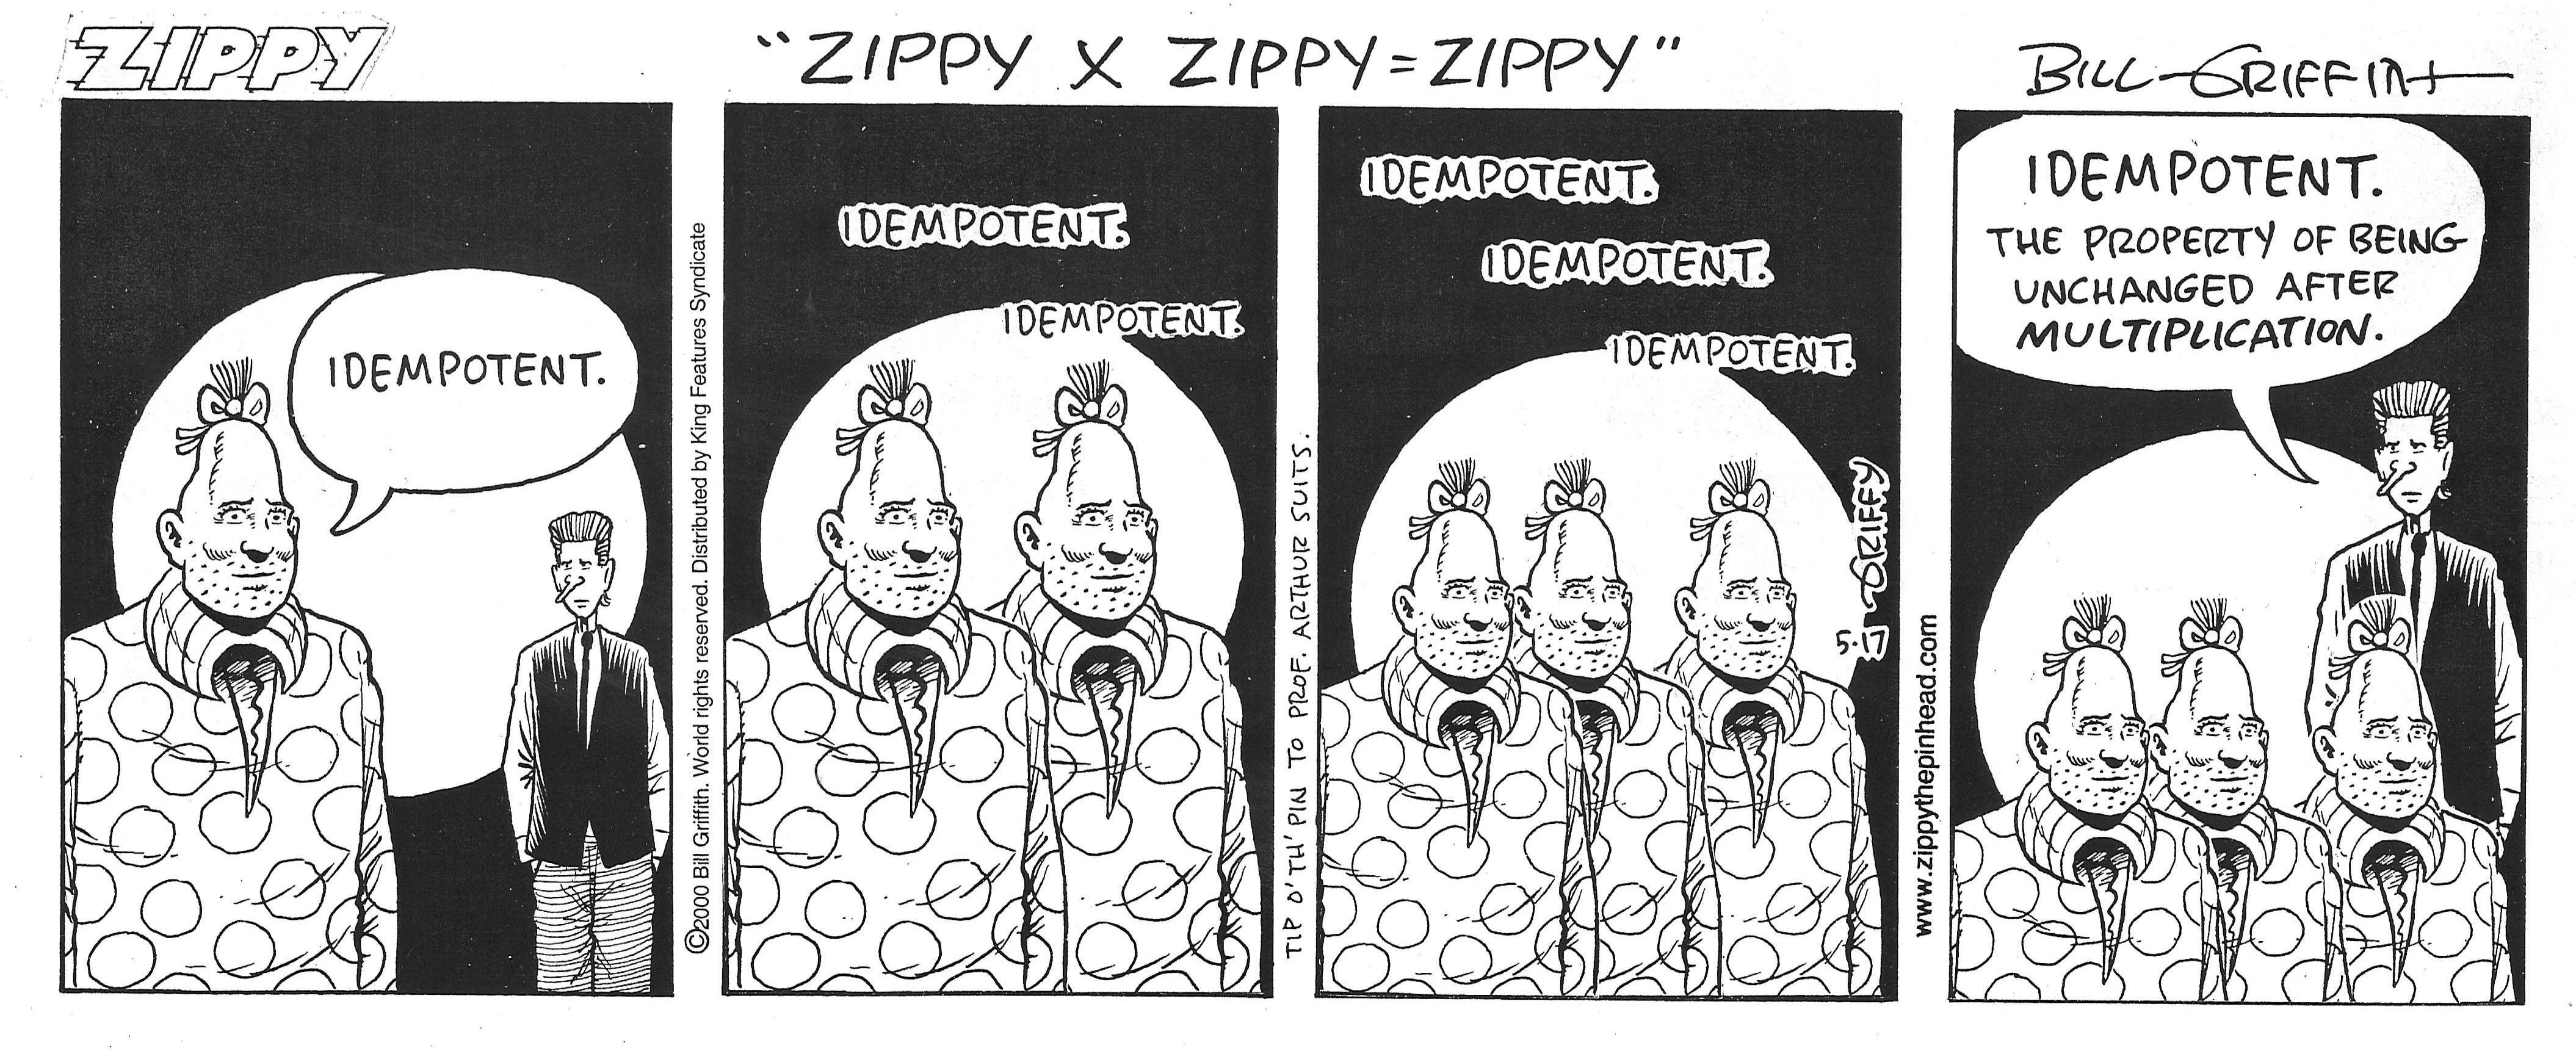
\includegraphics[width=\textwidth]{zippy.png}
{\small \copyright Bill Griffith. Reprinted with permission.}
             \end{center}

 \begin{solution}[print=true]
 Let $u,v\in H$.  To show $u*v\in H$, we need to show that $(u*v)*(u*v)=u*v$. Now,
 \begin{align*}
(u*v)*(u*v)&=u*(v*u)*v &&\text{(since $*$ is associative)}\\
&=u*(u*v)*v &&\text{(since $*$ is commutative)}\\
&=(u*u)*(v*v) &&\text{(since $*$ is associative)}\\
&=u*v &&\text{(since $u,v\in H$)}.
\end{align*} So $u*v\in H$.
 \end{solution}



\section{The definition of a group}

At this point you may be asking yourself, why do we care?  We've covered a lot of definitions and proved some theorems, but what is the goal of all this? Well, there are actually many goals that we can achieve using such material.  Consider the following as an example.  Suppose we want to solve the equation $5+x=2$.  We can probably solve this quite easily almost just by looking at it ($x=-3$), but what facts are we actually using there?  If we break down the reasoning leading to this answer, we may obtain something like the following set of steps.

\begin{center}
\begin{tabular}{rrlrl}&$5+x$ &=& $2$& \\
$\Rightarrow$ & $-5+(5+x)$ & = &$-5+2$& \\
$\Rightarrow$ & $(-5+5)+x$ & = &$-3$& \\
$\Rightarrow$ & $0+x$ &= &$-3$& \\
$\Rightarrow$ & $x$&=&$-3$&.
\end{tabular}
\end{center}
In line 2, we add the inverse of $5$ in $\<\Z, +\>$ to each side of
the equation.  In line 3, we use associativity of $+$ in $\Z$ (along
with computation), while in line 4 we use the fact that $-5$ is the
additive inverse of $5$ (that is, the inverse of $5$ in $\Z$ under
$+$).  Finally, in line 5 we use the fact that 0 is an additive
identity element in $\Z$ (that is, the identity element in $\Z$
under $+$).

In summary, we used \textbf{associativity, identity elements, and
inverses} in $\Z$ to solve the given equation. This perhaps
suggests that these would be useful traits for a binary
structure and/or its operation to have.  They are in fact so
useful that a binary structure displaying these characteristics
is given a special name. We note that these axioms are rather
strong; ``most" binary structures aren't groups.

\begin{df}{Definition and notation} A \textit{group} is a set $G$, equipped with a binary
operation $*$, that satisfies the following three \textit{group
axioms}:
\begin{enumerate}
\item[$\G_1$:] $*$ is associative on $G$;
\item[$\G_2$:] There exists an identity element for $*$ in $G$;
\item[$\G_3$:] Every element $a\in G$ has an inverse in $G$.
\end{enumerate}
\noindent We
    denote group $G$ under $*$ by the binary structure notation
    $\<G,*\>$, or simply by $G$ if the operation $*$ is known
    from context (or need not be known in the current
    situation).\end{df}

\fbox{\begin{minipage}{380pt}\begin{center}\begin{minipage}{360pt}\begin{center}
\medskip \textbf{
IMPORTANT NOTE}\end{center} When proving/disproving that a set $G$ is/is
not a group under an (apparent) operation $*$:

\begin{itemize}
\item The first thing you should do is check to make sure that  $\<G,*\>$
    is a binary structure by making sure $G$ is closed under $*$---if not, it doesn't make sense to
    check to see if axioms $\G_1$--$\G_3$ hold). (For instance: $\Z^*$ has no chance of being a group under
$\div$, since, e.g., $3,4\in \Z^*$ but $3 \div 4 \not\in\Z^*$.)

\item You should never check $\G_3$ before confirming
    $\G_2$ holds, because it makes no sense to look for
    inverses if you haven't confirmed that $G$ contains an
    identity element under $*$.

    \end{itemize}
   \smallskip
\end{minipage}\end{center}
\end{minipage}}


\section{Examples of groups/nongroups, Part I}
Let's look at some examples of groups/nongroups.

\begin{example}{}
We claim that $\Z$ is a group under addition.  Indeed, we already
know that $\Z$ is closed under addition and that addition is
associative on the integers.  The integer $0$ acts as an identity
element of $\Z$ under addition (since $a+0=0+a=a$ for each $a\in
\Z$), and each element $a$ in $G$ has inverse $-a$ since
$a+(-a)=-a+a=0$. \end{example}

\begin{example}{}\
\begin{enumerate}
\item  For each following binary structure $\<G,*\>$, determine whether or not $G$ is a group.
\item For those that are \textit{not\,} groups, determine the first group axiom  that fails, and provide a proof that it fails.

\item[]
\begin{center}
\begin{tabular}{p{1in}p{1in}p{1in}p{1in}}
$\<\fatq,+\>$ & $\<\Z,-\>$ & $\<\fatr,\cdot\,\>$ & $\<\fatc^*,\cdot\, \>$\\
$\<\fatr,+\>$ & $\<\Z^+,+\>$ & $\<\Z^*,\cdot\,\>$ & $\<\M_n(\fatr),+\>$\\
$\<\fatc,+\>$ & $\<\Z, \cdot\,\>$ & $\<\fatr^*,\cdot\, \>$ & $\<\M_n(\fatr),\cdot\, \>$
\end{tabular}
\end{center}
\end{enumerate}
\end{example}


\noindent If you have taken
linear algebra, you have also probably seen a collection of matrices
that is a group under matrix multiplication.


\begin{df}{Definitions} For $n\in \Z^+$, we define $GL(n,\fatr)$ by
$$GL(n,\fatr):=\{M\in \M_n(\fatr):\det M \neq 0\}.$$ In other
words, $G$ is the set of all invertible $n\times n$ matrices
over $\fatr$. We also define subset $SL(n,\fatr)$ of
$GL(n,\fatr)$, by
$$SL(n,\fatr):=\{M\in \M_n(\fatr):\det M =1\}.$$\end{df}

\begin{df}{Notation} We may use the notation $\0$ to denote a zero matrix and $I_n$ to denote an $n\times n$ identity matrix.\end{df}

\begin{df}{Remark} Throughout this course, if we are discussing a set $GL(n,\fatr)$ or $SL(n,\fatr)$, you should assume $n\in \Z^+$, unless otherwise noted.\end{df}

\begin{thm}\label{glsl} $GL(n,\fatr)$ and $SL(n,\fatr)$ are closed under matrix multiplication (so $\<GL(n,\fatr),\cdot\>$ and $\<SL(n,\fatr),\cdot\>$ are binary structures).\end{thm}

\begin{proof} Let $A,B\in GL(n, \fatr)$. Then $\det(AB)=(\det A)(\det B) \neq 0$ (since $\det A, \det B \neq 0)$, so $AB\in GL(n,\fatr)$.  Similarly, if $A,B \in SL(n,\fatr)$, then $\det(AB)=(\det A)(\det B)=1(1)=1$, so $AB\in SL(n,\fatr)$.\end{proof}

\begin{example}{} The binary structures
 $GL(n,\fatr)$ and $SL(n,\fatr)$ are groups under matrix multiplication.

\begin{proof} Let $G:=GL(n,\fatr)$. We show that $G$, under matrix multiplication, satisfies
the three group axioms.
\begin{enumerate}
\item[$\G_1$:] Matrix multiplication is always associative.
\item[$\G_2$:] The $n\times n$ identity matrix
    $$I_n:=\begin{bmatrix}
1 & 0 & 0 & \cdots & 0 \\
0 & 1 & 0 & \cdots & 0 \\
0 & 0 & 1 & \cdots & 0 \\
\vdots & \vdots & \vdots & \ddots & \vdots \\
0 & 0 & 0 & \cdots & 1 \end{bmatrix} \in G$$
acts as an identity element for $\<G, \cdot\,\>$ since $$AI_n=I_nA = A$$ for all $A\in G$.
\item[$\G_3$:] Let $A\in G$.  Since $\det A\neq 0$, $A$ has
    (matrix multiplicative) inverse $A^{-1}$ in
    $\M_2(\fatr)$. But we need to verify that $A^{-1}$ is in
    $G$. This is in fact the case, however, since
    $A^{-1}$ is invertible (it has inverse $A$), hence $\det
    A^{-1} \neq 0$.  Thus, $A^{-1}$ is also in $G$.
    \end{enumerate}

So $G$ is a group under multiplication.

\red{The proof that $SL(n,\fatr)$ is a group under multiplication is left as an exercise for the reader.}\end{proof} \end{example}

These groups are very important in many areas of mathematics, including linear algebra and geometry.  Because of this, we have special names for them (which give rise to the ``GL" and ``SL" in their names).

\begin{df}{Definitions} For $n\in \Z^+$, $GL(n,\fatr)$ is called the \textit{general
linear group of degree $n$ over $\fatr$} and $SL(n,\fatr)$ is
called the \textit{special linear group of degree $n$ over
$\fatr$}.\end{df}

\begin{example}{} Define $*$ on $\fatq^*$ by $a*b=(ab)/2$ for all $a,b\in \fatq^*$.  Prove that $\<\fatq^*,*\>$ is a group.

\begin{proof} First, $\fatq^*$ is closed under $*$, since $(ab)/2$ is
rational and nonzero whenever $a,b$ are rational and nonzero.

Next, we check that $\fatq^*$ under $*$ satisfies the group
axioms. Since multiplication is commutative on $\fatq$, $*$ is
clearly commutative on $\fatq^*$, and so our work to show
$\G_2$ and $\G_3$ is marginally reduced.

\begin{enumerate}
\item[$\G_1$:] Associativity of $*$ on $\fatq^*$ is inherited
    from associativity of multiplication on $\fatq^*$.
\item[$\G_2$:] Notice that the perhaps ``obvious" choice, 1, is
    \underline{not} an identity element for $\fatq^*$ under
    $*$: for instance, $1*3=3/2 \neq 3$. Rather, $e$ is such an
    identity element if and only if for all $a\in \fatq$ we
    have $a=e*a=(ea)/2$. We clearly have $a=(2a)/2$ for all
    $a\in \fatq^*$; so $2$ acts as an identity element for
    $\fatq^*$ under $*$.
\item[$\G_3$:] Let $a\in \fatq^*$.  Since $a\neq 0$, it makes
    sense to divide by $a$; then $4/a\in \fatq^*$, with
    $a*(4/a)=(a(4/a))/2=2$.
\end{enumerate}
Thus,  $\<\fatq^*,*\>$ is a group.\end{proof}
\end{example}

\section{Group conventions and properties}

\noindent Before we discuss more examples, we present a theorem and look at some conventions we follow and notation we use  when discussing groups in general; we also discuss some properties of groups.

\subsection{Some group conventions}
\smallskip

\begin{thm}\label{} The identity element of a group is
unique (by Theorem \ref{uniqueid}), and given any element $a$
of a group $G$, the inverse of $a$ in $G$ is unique (by Theorem
\ref{uniqueinverse}).\end{thm}


\begin{itemize}
\item
We usually \textbf{don't} use the notation $*$ when describing group
operations. Instead, we use the multiplication symbol $\cdot$ for
the operation in an arbitrary group, and  call
    applying the operation ``multiplying"---even though the operation may
not be ``multiplication" in the non-abstract, traditional sense! It may
    actually be addition of real numbers, composition of
    functions, etc.


Moreover, when actually operating in a group $\<G, \cdot\,\>$, we
typically omit the $\cdot$\,. That is, for $a,b\in G$, we write the
product $a\cdot b$ as $ab$. We call this the ``product" of $a$ and $b$. We will generally use $e$
or $e_G$ as our default notation for an identity element of group,\footnote{Many mathematicians denote a group's identity element by 1, rather than $e$.} and $a^{-1}$ to denote the inverse of element $a$ in $G$.

\bigskip
\warn{Although it is what we call \textit{multiplicative
notation} for an inverse, do \underline{not} assume $a^{-1}$ is what we usually think of as a
multiplicative inverse for $a$; remember, we don't even know if
elements of a group are numbers! The type of inverse that $a^{-1}$
is (a multiplicative inverse for a real number? an additive inverse
for a real number? a multiplicative inverse for a matrix? an inverse
function for a function from $\fatr$ to $\fatr$?) depends on both
$G$'s elements and its operation.}

\item For every element $a$ in a group $\Gdot$ and $n\in \Z^+$, we use the expression $a^n$ to denote  the product
$$\stackrel{\underbrace{a\cdot a \cdot \,\cdots \,\cdot a}}{n \mbox{ \rm times}}$$ and $a^{-n}$ to denote $(a^{-1})^n$ (that is, the product of $n$ copies of $a^{-1}$).
Finally, we define $a^0$ to be $e$.  Note that our ``usual" rules for exponents then hold in an arbitrary group: that is, if $a$ is in group $\<G, \cdot\,\>$
and $m,n\in \Z$, then $a^m a^n = a^{m+n}$ and $(a^m)^n=a^{mn}=(a^n)^m$.

\end{itemize}
\noindent
There are exceptions to these conventions:

\begin{itemize}
\item When working with an operation that is known to be commutative, we typically
continue to use additive notation ($+$ for the group operation, $-a$
for the inverse of element $a$ in the group) and call the operation
``addition," though using $\cdot$ is also valid in these cases. When
we use additive notation, we do \underline{not} omit the $+$ when
operating in a group $\<G,+\>$, and we call $a+b$ a \textit{sum} rather
than a product.\footnote{Also, when working with an operation that is known to be commutative, the identity element may be denoted by 0 rather than by $e$, $e_G$, or 1.}  For $n\in \Z^+$, we write $na$ instead of $a^n$; we also write $0a$ instead of $a^0$. Finally, note that
$(-n)a=n(-a)=-(na)$ (where $-a$ and $-(na)$ indicate the
additive inverses of $a$ and $na$, respectively); we can therefore
unambiguously use the notation $-na$ for this element.
Using this notation, note that for $m\in \Z$, $na+ma=(n+m)a$ and $n(ma)=(nm)a$.

\bigskip
\warn{Be careful to always know where an element
you are working with lives!  For instance, if, as above, $n\in
\Z^+$ and $a$ is a group element, $-n$ and $-a$ look similar but
may mean very different things.  While $-n$ is a negative integer,
$-a$ may be the additive inverse of a matrix in $\M_2(\fatr)$, the
additive inverse 2 of the number 4 in $\Z_6$, or even something
completely unrelated to numbers.}

We summarize multiplicative versus addition notation in the following table, where $a,b$ are elements of a group $G$.


\begin{center}
\begin{threeparttable}
\renewcommand{\arraystretch}{1.3}
\begin{tabular}{|l|c|c|}
\hline
 & \textbf{Multiplicative notation\tnote{*}}& \textbf{Additive notation\tnote{$\dagger$}}\\
\hline
Operation notation& $\cdot$ & +\\
$a$ operated with $b$ & product $ab$ & sum $a+b$\\
Identity element & 1 (or $e$ or $e_G$) & 0 (or $e$ or $e_G$)\\
Inverse of $a$ & $a^{-1}$ & $-a$\\
\hline
\end{tabular}

\begin{tablenotes}
\item[*]\small Used in an arbitrary group.
\item[$\dagger$]\small Used only in abelian groups.
\end{tablenotes}
\end{threeparttable}
\end{center}


\item We \textbf{do} use the notation
$*$ when using multiplicative or additive notation would lead to
confusion. For instance, if we want to define an operation on
$\fatq^*$ that assigns to pair $(a,b)$ the quantity $ab/2$, it would
be unwise to use multiplicative or additive notation for this
operation since we already have conventional meanings of $ab$ and
$a+b$. Similarly, we would not denote the identity element of
$\fatq^*$ under this operation by $0$ or $1$, since the identity
element in this group is the rational number $2$, and writing $0=2$
or $1=2$ would look weird.

\item If there is a default notation for a particular
operation (say, $\circ$ for composition of functions) or identity
element (say, $I_n$ in $GL(n,\fatr)$) we usually use that notation
instead.

\end{itemize}

\subsection{Some group properties}
\bigskip
While we don't need to worry about ``order" when multiplying a group element $a$ by itself, we \textbf{do} need to worry about it in general.

\bigskip
\warn{\begin{center}Group operations need \textit{not} be commutative!\end{center}}

\begin{df}{Definitions} A group $\<G, \cdot\,\>$ is said to be \textit{abelian}\footnote{
The word ``abelian" is derived from the surname of
mathematician Niels Henrik Abel.} if $ab=ba$ for all $a,b\in
G$. Otherwise, $G$ is \textit{nonabelian}.\end{df}

\begin{df}{Remark} If we know that a binary operation $\cdot$
on a set $G$ is commutative, then in checking to see if axioms
$\G_2$ and $\G_3$ hold we need only verify that there exists
$e\in G$ such that $ae=a$ (we don't need to check that
$ea=a$) for all $a\in G$ and that for each $a\in G$ there
exists $b\in G$ such that $ab=e$ (we don't need to check that
$ba=e$).\end{df}

\begin{df}{Remark} If $G$ is not known to be abelian, we
must be careful when multiplying elements of $G$ by one
another: multiplying on the left is, in general, not the same
as multiplying on the right! \end{df}

\begin{df}{Definitions} If $G$ is a group, then the cardinality $|G|$ of $G$ is
called the \textit{order of $G$}. If $|G|$ is finite, then $G$ is
said to be a \textit{finite group}; otherwise, it's an \textit{infinite group}.\end{df}


\begin{example}{} Of the groups we've discussed, which are abelian? Which are infinite/finite?\end{example}

We have already seen that identity elements of groups are unique,
and that each element $a$ of a group $G$ has a unique inverse
$a^{-1}\in G$. Here are some other basic properties of groups.
\begin{thm}\label{cancel} If $\Gdot$ is a group, then \emph{\textbf{left and right cancellation laws}} hold in $G$.  That is, if $a,b,c\in G$, then

\begin{center}\begin{enumerate} \item If $ab=ac$, we have $b=c$ (the left cancellation law); and
\item If $ba=ca$, we have $b=c$ (the right cancellation law).\end{enumerate}
\end{center}
\end{thm}

 \begin{proof} Let $a,b,c\in G$ and assume that $ab=ac$.  Multiplying
both equation sides on the left by $a^{-1}$, we obtain
\begin{alignat*}{2}
&& a^{-1}(ab)&=a^{-1}(ac)\\
  &\Rightarrow\quad
  &(a^{-1}a)b&=(a^{-1}a)c\\
  &\Rightarrow
  &eb&=ec\\
   &\Rightarrow
  &b&=c
\end{alignat*}
This proves that the left cancellation law holds.  A similar proof shows that the right cancellation law holds.\end{proof}

\begin{thm}\label{uniquesols} Let $\Gdot$ be a group and let $a,b\in G$. Then there exist \emph{\textbf{unique}} elements $x,y\in G$ such that $ax=b$ and $ya=b$.
\end{thm}


\begin{proof} If $x=a^{-1}b$ and $y=ba^{-1}$, then
$ax=a(a^{-1}b)=(aa^{-1})b=eb=b$ and
$ya=(ba^{-1})a=b(a^{-1}a)=be=b$. So such elements $x$ and $y$
exist.  The fact that they are unique follows from the cancellation
laws: if $ax=b$ and $ax'=b$ then $x=x'$ by left cancellation, and
if $ya=b$ and $y'a=b$ then $y=y'$ by right cancellation.\end{proof}

\warn{\begin{center}We only of necessity have $(ab)^{-1}=a^{-1}b^{-1}$ if $G$ is known to be abelian!\end{center}}

However, we do have the following:

\begin{thm}\label{invofprod} If $a$ and $b$ are elements of a group $\Gdot$, then $$(ab)^{-1}=b^{-1}a^{-1}.$$
\end{thm}

\begin{proof} We have that
$$(ab)(b^{-1}a^{-1})=a(bb^{-1})a^{-1}=aea^{-1}=aa^{-1}=e.$$
Similarly, $(b^{-1}a^{-1})(ab)=e$.\end{proof}
\section{Examples of groups/nongroups, Part II}

\begin{example}{} Let $n\in \Z^+$.  We define $n\Z$ by $$n\Z=\{nx: x\in \Z\}:$$ that is, $n\Z$ is the set of all (integer) multiples of $n$.

\begin{thm}\label{nz} $n\Z$ is a group under $+$ (the usual addition of integers).\end{thm}

\begin{proof} Let $x, y\in n\Z$. Then there exist $a,b\in \Z$ such that $x=na$ and $y=nb$.  Then $x+y=na+nb=n(a+b)\in n\Z$. So $\<n\Z,+\>$ is a binary structure.  \red{The remainder of the proof is left as an exercise for the reader.}\end{proof}
\end{example}

\begin{df}{Remark} When we are discussing a group $n\Z$, assume that $n\in \Z^+$, unless otherwise noted.\end{df}

 We use an  example from our next class of groups all the time;
in fact, most six-year-olds do as well, since it is used when
telling time! Before we get to the example, we need some more
definitions and some notation. Throughout the following discussion,
assume $n$ is a fixed positive integer.

\begin{df}{Definitions and notation} We say integers $a$ and $b$ are \textit{congruent
modulo [or mod] $n$} if $n$ divides $a-b$. If $a$ and $b$ are
congruent mod $n$, we write $a \equiv b\, \pmod{n}$.\end{df}

\begin{example}{cong.ex} $1, 7, 13,$ and $-5$ are all congruent mod $6$. \end{example}

The following is a profoundly useful theorem; it's so
important, it has a special name. We omit the proof of this theorem,
but direct interested readers to for, instance, p. 5 in \cite{NZM}.

\begin{df}{The Division Algorithm} Let $n\in \Z^+$ and let $a$ be any
integer.  Then there exist unique integers $q$ and $r$, with $0\leq
r <n$, such that $a=qn+r$.\footnote{This is actually a special case
of a more general theorem, which states that given any integers $n$
and $a$, there exist unique integers $q$ and $r$, with $0\leq
r<|n|$, such that $a=qn+r$.}\end{df}

 It follows that for each positive integer $n$ and integer $a$,
there exists a unique element $R_n(a)$ (the $r$ in the above
theorem) of the set $\{0,1,2,\ldots, n-1\}$ such that $a$ is
congruent to $R_n(a)$ modulo $n$. For example, $R_3(4)=1$, $R_3(0)=0$,
$R_3(17)=2$, and $R_3(-5)=1$.


\begin{df}{Definition} $R_n(a)$ is the \textit{remainder} when we divide $a$ by $n$. (Note: You were probably already familiar with the remainder when you divide a \textbf{positive} integer by $n$.)\end{df}

\begin{df}{Definition} We define \textit{addition modulo $n$}, $+_n$, on $\Z$ by,
for all $a,b\in \Z$,
$$a+_n b=R_n(a+b),$$ that is, the unique element of $\{0,1,\ldots, n-1\}$ that's congruent to the integer $a+b$ modulo $n$.\end{df}


\begin{df}{Remark} Addition mod 24 is what we use to tell
time!\end{df}

 The set $\{0,1,2,\ldots, n-1\}$ of remainders when dividing by $n$ is so important we give it a
special notation.


\begin{df}{Notation} We denote by $\Z_n$ the set $\{0,1,2,\ldots,n-1\}$.\end{df}

Throughout this course, if we are discussing a set $\Z_n$, you
should assume $n\in \Z^+, n\geq 2$, unless otherwise noted.
(Though it will rarely come up for us, we may occasionally make
reference to $\Z_1=\{0\}$.)

\bigskip
\warn{\begin{center}Note that by our definition of $\Z_n$, the
integer $n$ itself is \underline{not} in $\Z_n$!\end{center}}


 We are now ready to consider our next type of group.

\begin{example}{} For each $n\in \Z^+$, $\<\Z_n,+_n\>$ is a group, called the \textit{cyclic group of order $n$} (we will see later why we use the word ``cyclic" here).
This group is abelian and of order $n$.

\begin{proof} We first check that $\Z_n$ is closed under $+_n$. Note
that by the definition of $+_n$, $a+_nb \in \Z_n$ for each
$a,b\in \Z$.  Thus, $a+_nb \in \Z_n$ for each $a,b\in \Z_n$.

We next check that $\Z_n$ under $+_n$ satisfies the three group
axioms. Note that since addition is commutative on $\Z$, $$a+_n
b =R_n(a+b)=R_n(b+a)=b+_n a$$ for all $a,b\in \Z_n$. Again, a
simpler way of stating this is that commutativity of $+_n$ on
$\Z_n$ is inherited from the commutativity of addition on $\Z$.
One nice result of this is that since $+_n$ is commutative on
$\Z_n$, we have less to check when verifying group axioms
$\G_2$ and $\G_3$.

\begin{enumerate}
\item[$\G_1$:]  Let $a,b,c\in \Z_n$.  We want to show that
    $(a+_n b)+_n c = a +_n(b+_n c)$. Now,
\begin{comment}
\begin{eqnarray*}
(a+_n b)+_n c&=& R_n(a+b)+_n c\\
&\equiv& (R_n(a+b)+c) \pmod n \\
&\equiv& ((a+b)+c) \pmod n\\
&\equiv& (a+(b+c)) \pmod n\\
&\equiv& (a+R_n(b+c)) \pmod n \\
&\equiv& a+_n (b+_n c) \pmod n.
\end{eqnarray*}
\end{comment}
\begin{align*}
(a+_n b)+_n c&=R_n(a+b)+_n c&&\\
&\equiv R_n(a+b)+c&& \pmod n \\
&\equiv (a+b)+c&&  \pmod n\\
&\equiv a+(b+c)&&  \pmod n\\
&\equiv a+R_n(b+c)&&  \pmod n \\
&\equiv a+_n (b+_n c)&& \pmod n.
\end{align*}


So $(a+_n b)+_n c$ and $a+_n (b+_n c)$ are congruent mod $n$.  Since
both of these values are in $\{0,1,\ldots, n-1\}$, this implies that
they are equal, as desired.
\item[$\G_2$:] Clearly, $0\in \Z_n$ acts as an identity element
    under $+_n$, since $$0+_n a =R_n(0+a)=R_n(a)$$ for each
    $a\in \Z_n$.
\item[$\G_3$:] Let $a\in \Z_n$.  If $a=0$, then clearly $a$ has
    inverse $0\in \Z_n$ since $0+_n 0 = 0$. If $a\neq 0$, then
    the element $n-a\in \Z_n$ is an inverse for $a$ since
    $$a+_n(n-a)=R_n(a+(n-a))=R_n(n)=0.$$
 \end{enumerate}

Since $+_n$ is commutative on $\Z_n$, $\Z_n$ is an abelian  group under $+_n$.  Finally, we already know that $|\Z_n|=|\{0,1,2,\ldots,n-1\}|=n$.\end{proof}
\end{example}

\begin{df}{Remark} In practice, we often omit the
subscript $n$ and just write $+$ when discussing addition
modulo $n$ on $\Z_n$.\end{df}

\warn{\begin{center}Do not confuse $n\Z$ and $\Z_n$! They are very different as sets and as groups.\end{center}}


\begin{example}{} In the group $\<\Z_8,+\>$ (where, as indicated by our above remark, $+$ means addition modulo $8$), we have, for instance, $3+7=2$ and $7+7=6$.
The numbers 2 and 6 are each other's inverse, and $7^{-1}=1$. The number $0$ has inverse $0$ (it can't be $8$, since $8\not\in \Z_8$!). \end{example}

\begin{df}{Definition} For $n\in \Z^+$,  we define binary operation $\cdot_n$ (\textit{multiplication modulo $n$}) on $\Z_n$ by $a\cdot_n b = r_n(a)$, the remainder when $ab$ is divided by $n$.\end{df}

\begin{df}{Remark} $\Z_n$ is never a group under $\cdot_n$ (do you see why?). \end{df}

But we can consider the following

\begin{df}{Definition} For $n\in \Z^+$,
let $\Z_n^{\times} = \{a\in \Z_n\,:\,\gcd(a,n)=1\}$.\end{df}

\begin{example}{}
$\<\Z_n^{\times},\,\cdot\, \>$ is a group under multiplication.  We omit the proof. \end{example}

We end by considering a few more examples.

\begin{example}{} Let $F$ be the set of all functions from $\fatr$ to $\fatr$, and define \textit{pointwise addition} $+$ on $F$ by
$$(f+g)(x)=f(x)+g(x)$$ for all $f,g\in F$ and $x\in \fatr$. We claim that $F$ is a group under pointwise
addition. (For variety, in this proof we don't explicitly refer
to $\G_1$--$\G_3$, though we certainly do verify they hold.)
Indeed, if $f,g\in F$ then clearly $f+g$ is also a function
from $\fatr$ to $\fatr$, so $F$ is closed under $+$.

Next, let $f,g,h\in F$.  Then for all $x\in \fatr$,
\begin{align*}
((f+g)+h)(x)&=(f+g)(x)+h(x)&&\\
&=((f(x)+g(x))+h(x)&&\\
&=f(x)+(g(x)+h(x))&&\text{(since addition is associative on
$\fatr$)}\\
&=f(x)+(g+h)(x)&&\\
&=(f+(g+h))(x)&&.\end{align*} Note
that the key fact used in this argument is that $f(x)$, $g(x)$ and
$h(x)$ all lie in $\fatr$, and addition is associative on $\fatr$.
When you get used to such arguments, it is sufficient to say that
associativity of $+$ on $F$ is \textit{inherited} from the
associativity of addition on $\fatr$.

Next, let $z:\fatr\to\fatr$ be the function $z(x)=0$ for all $x$.  Then for all $f\in F$ and $x\in \fatr$, $$(f+z)(x)=f(x)+z(x)=f(x)+0=f(x)=0+f(x)=z(x)+f(x)=(z+f)(x).$$ So $z$ is an identity element of $\<F,+\>$.

Finally, let $f\in F$, and define $g\in F$ by $g(x)=-f(x)$ for all $x\in \fatr$.  It is easy then to see that $g$ is an inverse for $f$ in $F$.

Hence, $F$ is a group under pointwise addition. Note that it is uncountably infinite and abelian. \end{example}

\begin{example}{}The set $F$ is \textbf{not} a group under function composition (do you see why?). But if we define $B$ to be the set of all \textbf{bijections} from $\fatr$ to $\fatr$, then $B$ is a group under function composition. (Prove it!) $B$ is uncountably infinite and nonabelian. \end{example}

\begin{example}{gpprod}
Let $\<G_1,*_1\>$, $\<G_2,*_2\>$ , $\ldots$, $\<G_n,*_n\>$ be groups ($n\in \Z^+$).  Then the \textit{group product}
$$G=G_1\times G_2\times \cdots \times G_n$$ is a group under the \textit{componentwise} operation $*$ defined by
$$(g_1,g_2,\ldots, g_n)*(h_1,h_2,\ldots,h_n)=(g_1*_1h_1, g_2*_2h_2,\ldots, g_n*_nh_n)$$ for all $(g_1,g_2,\ldots, g_n),(h_1,h_2,\ldots,h_n)\in G$.

\bigskip
For instance, considering multiplication on $\fatr^*$, matrix multiplication on $GL(2,\fatr)$, and addition modulo $6$ on $\Z_6$, we have that $\<\fatr^*\times GL(2,\fatr) \times \Z_6,*\>$ is a group in which, for instance, $$\left(-1, \left[
                                                                         \begin{array}{cr}
                                                                           1 & 3 \\
                                                                           0 & -1 \\
                                                                         \end{array}
                                                                       \right],
                                                                       3\right)
                                                                       *\left(\pi,
                                                                       \left[
                                                                         \begin{array}{cc}
                                                                           2 & 1 \\
                                                                           1 & 1 \\
                                                                         \end{array}
                                                                       \right],4\right)=\left(-\pi, \left[
                                                                         \begin{array}{rr}
                                                                           5 & 4 \\
                                                                           -1 & -1 \\
                                                                         \end{array}
                                                                       \right],1\right).  $$
                                                                       \end{example}

\begin{example}{}
A common example of a group product is the group $\Z_2^2$, equipped with componentwise addition modulo 2. \end{example}

\begin{df}{Definition} The group $\Z_2^2$ is known as the \textit{Klein 4-group}.\footnote{Felix Klein was a German mathematician; you may have heard of him in relation to the Klein Bottle. You may see the group $\Z_2^2$ denoted by $V$, for ``Vierergruppe," the German word for "four-group".} \end{df}

\section{Summaries of groups we've seen}
When you see the following identified as groups, you should
assume they are equipped with the following operations, unless
otherwise. Throughout, assume $m,n\in \Z^+$.
\begin{center}
\begin{threeparttable}
\renewcommand{\arraystretch}{1.3}
\begin{tabular}{|l|l|l|} \hline \textbf{Group(s)} &\textbf{Operation}&
\textbf{Properties} \\\hline $\Z$, $\fatq$ & addition of numbers & countably
infinite; abelian%; cyclic
\\\hline $n\Z$ &  addition of numbers
& countably infinite; abelian\tnote{*}%;cyclic
\\\hline $\fatr$, $\fatc$ & addition of numbers&
uncountable; abelian%; noncyclic
\\\hline $\fatq^*$, $\fatq^+$ &
multiplication of  numbers& countably infinite; abelian%;noncyclic
\\\hline $\fatr^*$, $\fatr^+$, $\fatc^*$ &
multiplication of  numbers& uncountable; abelian%; noncyclic
\\\hline
$\M_{m\times n}(\fatr), \M_n(\fatr)$ & matrix addition &
uncountable; abelian%; noncyclic
\\\hline $GL(n,\fatr), SL(n,\fatr)$ &
 matrix multiplication& uncountable; nonabelian\tnote{$\dagger$}%;noncyclic
\\\hline $\Z_n$ & addition mod $n$  & finite; abelian%;cyclic
\\\hline $\Z_2^2$& componentwise addition mod 2& finite; abelian%; noncyclic
\\\hline $F$& pointwise addition& uncountable; abelian
\\ \hline$B$&composition&uncountable; nonabelian\\
\hline
\end{tabular}
\begin{tablenotes}
\item[*]\small Unless $n=0$.
\item[$\dagger$]\small Unless $n=1$.
\end{tablenotes}
\end{threeparttable}
\end{center}


\pagebreak
\section{Exercises, Part II}

\begin{exercise}[ID=2A]
\tf

\begin{enumerate}
\item For every positive integer $n$, there exists a group of order $n$.

\item For every integer $n\geq 2$, $\Z_n$ is abelian.

\item Every abelian group is finite.

\item For every integer $m$ and integer $n>2$, there exist infinitely many integers $a$ such that $a$ is congruent to $m$ modulo $n$.

\item A binary operation $*$ on a set $S$ is commutative if and only if there exist $a,b\in S$ such that $a*b=b*a$.

\item If $\<S, *\>$ is a binary structure, then the elements of $S$ must be numbers.

\item If $e\in \<S,*\>$ is an identity element of $S$, then $e$ is an idempotent in $S$ (that is, $e*e=e$).

\item If $s\in \<S,*\>$ is an idempotent, then $s$ must be an identity element of $S$.
\end{enumerate}
\end{exercise}

\begin{solution}[print=true]


\noindent
\begin{inparaenum}[(a)]
\item T \hfill \item T  \hfill \item  F  \hfill \item T  \hfill \item F  \hfill \item F  \hfill \item T   \hfill\item F
\end{inparaenum}

\end{solution}


\begin{exercise}[ID=2F]
Let $G$ be the set of all functions from $\Z$ to $\fatr$.  Prove that pointwise multiplication on $G$ is commutative. (\textbf{Note.} To prove that two functions, $h$ and $j$, sharing the same domain $D$ are equal, you need to show that $h(x)=j(x)$ for every $x\in D$.)
\end{exercise}

\begin{solution}[print=true]
Let $f,g\in G$.  Then for every $x\in \Z$,
$$(fg)(x)=f(x)g(x)=g(x)f(x),$$
since $f(x), g(x)\in \fatr$ and multiplication of real numbers is commutative. Since $g(x)f(x)=(gf)(x)$,
$fg=gf$, and so pointwise multiplication on $G$ is commutative.
\end{solution}

\begin{exercise}[ID=2J]
Decide which of the following binary structures are groups.  For each, if the binary structure \textit{isn't} a group, prove that. (Remember, you should \textit{not} state that inverses do or do not exist for elements until you have made sure that the structure contains an identity element!) If the binary structure {\it is} a group, prove that.

\begin{enumerate}
\item $\fatq$ under multiplication
\item $\M_2(\fatr)$ under addition
\item $\M_2(\fatr)$ under multiplication
\item $\fatr^+$ under $*$, defined by $a*b=\sqrt{ab}$ for all $a,b\in \fatr^+$
\end{enumerate}
\end{exercise}

\begin{solution}[print=true]
\begin{enumerate}
\item $\fatq$ isn't a group under multiplication since $0\in \fatq$ has no inverse.
\item
\begin{enumerate}
\item[$\G_1$:] Matrix multiplication is always associative.
\item[$\G_2$:] The zero matrix in $\M_2(\fatr)$ acts as an additive identity element.
\item[$\G_3$:] Let $A\in \M_2(\fatr)$.  Then $-A\in \M_2(\fatr)$ is an inverse for $A$ under addition.
\end{enumerate}
Thus, $\M_2(\fatr)$ is a group under addition.

\item $\M_2(\fatr)$ isn't a group under multiplication since the zero matrix has no inverse.
\item $1*(4*9)=1*6=\sqrt{6}$ while $(1*4)*9=2*9=\sqrt{18}$, so $*$ isn't associative.  Thus, $\fatr^+$ isn't a group under $*$.
\end{enumerate}
\end{solution}

\begin{exercise}[ID=2K]
Give an example of an abelian group containing 711 elements.
\end{exercise}

\begin{solution}[print=true]
$\Z_{711}$. (Other answers are possible.)
\end{solution}



\begin{exercise}[ID=2M]
Let $n\in \Z$.   Prove that $n\Z$ is a group under the usual addition of integers. \textbf{Note:} You may use the fact that $\<n\Z,+\>$ is a binary structure if you provide a reference for this fact.
\end{exercise}

\begin{solution}[print=true]
We know from Theorem \ref{nz} that $\<n\Z,+\>$ is a binary structure.

\begin{enumerate}
\item[$\G_1$:] $+$ is
    associative on $n$, since it's associative on
    $\Z$, and $n\Z \subseteq \Z$.

\item[$\G_2$:] Notice that
    $0\in n\Z$ (since $0=n(0)$); 0 then clearly acts as
    an identity element for $+$ in $n\Z$.

\item[$\G_3$:] Let $x\in n\Z$, then $x=nm$ for some $m\in \Z$, so
    $-x=n(-m)$ for $m\in \Z$, implying $-x\in n\Z$;
    and clearly $-x$ acts as an inverse for $x$ in
    $n\Z$.

    \end{enumerate}Thus, $\<n\Z, +\>$ is a group.

    \end{solution}

\begin{exercise}[ID=2N]
 Let $n\in \Z^+$. Prove that $SL(n,\fatr)$  is a group under matrix multiplication.
\textbf{Note:} You may use the fact that $\<SL(n\fatr),\cdot\>$ is a binary structure if you provide a reference for this fact.
\end{exercise}


\begin{solution}[print=true]
We know from Theorem \ref{glsl} that $\<SL(n,\fatr),\cdot\>$ is a binary structure.

\begin{enumerate}
\item[$\G_1$:] Matrix multiplication is always associative.

\item[$\G_2$:] Since $\det I_n=1$, $I_n$ is in $SL(n,\fatr)$, and clearly acts as an identity element in $SL(n,\fatr)$.

\item[$\G_3$:] Let $A\in SL(n,\fatr)$.  Since $\det A=1\neq 0$, $A$ has an inverse matrix $A^{-1}$ in $GL(n, \fatr)$.  $A^{-1}$ is in $SL(n,\fatr)$ since $$\det(A^{-1})=\frac{1}{\det A}=1/1=1.$$ So $A$ has an inverse in $SL(n,\fatr)$.
\end{enumerate}
Thus, our proof is complete.
\end{solution}


\begin{exercise}[ID=2P]
\begin{enumerate}
\item List three distinct integers that are congruent to $6$ modulo $5$.
\item List the elements of $\Z_5$.
\item Compute: \begin{enumerate}
\item $4+5$ in $\Z$;
\item $4+5$ in $\fatq$;
\item $4+_65$ in $\Z_6$;
\item the inverse of $4$ in $\Z$;
\item the inverse of $4$ in $\Z_6$.
\end{enumerate}
\item Why does it not make sense for me to ask you to compute $4+_3 2$ in $\Z_3$? \textbf{Please answer this using a complete, grammatically correct sentence.}

\end{enumerate}
\end{exercise}

\begin{solution}[print=true]
\begin{enumerate}
\item $11, 1, -4$. (Other answers are possible.)
\item  $\Z_5=\{0,1,2,3,4\}$
\item (i) 9 \quad (ii) 9 \quad (iii) 3 \quad (iv) $-4$ \quad (v) 2
\item It doesn't make sense because $4\not\in \Z_3$.
\end{enumerate}
\end{solution}


\begin{exercise}[ID=2O]
Let $G$ be a group with identity element $e$.  Prove that if every element of $G$ is its own inverse, then $G$ is abelian.

\end{exercise}

\begin{solution}[print=true]
Let $a,b\in G$.  Then
\begin{align*}ab&=(ab)^{-1}&&\text{(since $ab$
is its own inverse)}\\
&=b^{-1}a^{-1}&&\\
&=ba &&\text{(since $b$ and $a$ are their own
inverses)}.\end{align*} So $G$ is abelian.
\end{solution}


\begin{exercise}[ID=2R, subtitle=(Extra Credit)]
Let $G$ be a group.  The subset $$Z(G):=\{z \in G\,:\, zg=gz \mbox{ for all }g\in Z(G)\}$$ of $G$ is called the \textit{center} of $G$. In other words, $Z(G)$ is the set of all elements of $G$ that commute with every element of $G$.
Prove that $Z(G)$ is closed in $G$. %NOTE: This is actually proved in the chapter on Factor Groups.
\end{exercise}

\begin{solution}[print=true]
Let $z_1, z_2\in Z(G)$.  Let $z=z_1z_2$; we want to
show that $z$ is in $H$: that is, we want to show that for every $g\in G$,
$zg=gz$.  But for every $g\in G$,
\begin{center}
\begin{align*}
zg&=(z_1z_2)g&& \text{(using the definition of $z$)}\\
&=z_1(z_2g)&& \text{(since $G$'s operation is associative)}\\
&=z_1(gz_2)&& \text{(since $z_2\in Z(G)$)}\\
&=(z_1g)z_2 && \text{(since $G$'s operation is associative)}\\
&=(gz_1)z_2 && \text{(since $z_1\in Z(G)$)}\\
&=g(z_1z_2)&&  \text{(since $G$'s operation is associative)}\\
&=gz && \text{(using the definition of $h$)}.
\end{align*}\end{center}
Thus, $Z(G)$ is closed in $G$.

\end{solution} 
\chapter{Homorphisms and Isomorphisms}\label{homoiso}

\section{Groups of small order}

Let's start exploring groups in order of increasing, well, order. Before we do this, it will be helpful to introduce the notion of a \textit{group table} (also known as a {\it Cayley table}\footnote{Named after the British mathematician Arthur Cayley.}) for a finite group.  Given a finite group $G$, list its elements in some fixed order, say, $a_1, a_2, \ldots, a_n$, and then construct its group table by creating an array with exactly one row and exactly one column corresponding to each group element.  We then put in the row $i$ and column $j$ the element $a_ia_j$ of $G$.  Note that a single group can have group tables that look different from one another, since reordering a group's elements will change its table.


\begin{example}{}
Consider the group $\Z_4$ under addition modulo 4.  Ordering the elements of $\Z_4$ as $1,2,3,4$, we have the following group table for $\<\Z_4,+\>$:

\bigskip
\hspace{137pt}
\renewcommand{\arraystretch}{1.3}
$\begin{array}{c||c|c|c|c}
+&0&1&2&3\\ \hline\hline 0&0&1&2&3\\ \hline
1&1&2&3&0\\ \hline 2&2&3&0&1\\ \hline 3&3&0&1&2\\

\end{array}$

\vspace{-9pt}
\hspace{250pt}
\end{example}


Now, clearly, there is no group of order 0 (do you see why?).  Is there a group of order 1?  Well, suppose $\<G,*\>$ is such a group. Since $G$ must contain an identity element $e$, we must have $G=\{e\}$, and since $e$ is $G$'s identity element, we must have $e*e=e$.  Clearly, in this case, the three group axioms hold.  So $G$ is a valid group, without much going on in it.

\begin{df}{Definition} If $G$ is a group with $|G|=1$, then $G$ is called the
\textit{trivial group}\footnote{ A good question to ask here is
why it's called ``the" trivial group, rather than ``a" trivial
group.  Indeed, there are infinitely many groups of order 1!
(Do you see why?) But it turns out that all of these groups are
\textbf{structurally} the same. Hence mathematicians end up
thinking of them as various instantiations of one group, rather
than separate groups. We will discuss this in more depth
shortly, when we introduce the idea of \textit{isomorphism}.}.
\end{df}


Next suppose that group $\Gdot$ has order 2.  Then $G$ must contain an identity element, $e$, and a non-identity element, $a$.  Since $e$ is its own inverse, and inverses are unique, $a$ must be its own inverse as well.  So $G$ must have the following table.
\bigskip

\begin{center}
\renewcommand{\arraystretch}{1.3}
$\begin{array}{c||c|c}
*&e&a\\ \hline\hline e&e&a\\ \hline
a&a&e\\
\end{array}$
\end{center}

\bigskip

It is straightforward to show that such a structure does satisfy all the group axioms (the only one we really need to check is associativity).

Now, what if group $\Gdot$ has order 3?  Note that \textbf{you can't have any entry appear more than once in the same row or same column} (excluding of course the labels outside the grid we're filling in), given Theorem \ref{uniquesols}. Is there only one way of filling in the table for a group of order 3? (Hint: consider what element must be the second row, third column entry.)

\bigskip
\begin{center}
%\begin{tabular}{lr}
\renewcommand{\arraystretch}{1.3}
$\begin{array}{c||c|c|c}
*&e&a&b\\ \hline \hline e&&&\\ \hline
a&&&\\ \hline b&&&\\
\end{array}$
%&
%\renewcommand{\arraystretch}{1.3}
%$\begin{array}{c||c|c|c|c}
%*&e&a&b&c\\ \hline \hline e&&&&\\ \hline
%a&&&&\\ \hline b&&&&\\ \hline c&&&&\\
%\end{array}$\\
%\end{tabular}
\end{center}
\bigskip

Finally, what if group $\Gdot$ has order 4?  It turns out in this case there are \textbf{two} valid ways of filling in a group table!
%Hint: the group tables for $\Z_4$ and $\Z_2 \times \Z_2$, under the obvious operations, are structurally distinct.

\medskip
What we have been doing here is really getting into the idea of the
\textbf{structure} of groups, and when we can consider groups to be
essentially ``the same" or fundamentally ``different."  We approach
this more formally via the concepts of homomorphism and isomorphism.

\bigskip
\section{Introduction to homomorphisms and isomorphisms}

\begin{df}{Definitions} Let $\<S,*\>$ and $\<S',*'\>$ be binary structures.  A
function $\phi$ from $S$ to $S'$ is a \textit{homomorphism} if
$$\phi(a* b)=\phi(a)*'\phi(b)$$ for all $a,b\in S$. An \textit{isomorphism} is a homomorphism that is also a bijection.\end{df}

Intuitively, you can think of a homomorphism $\phi$ as a
``structure-preserving" map: if you multiply and then apply $\phi$,
you get the same result as when you first apply $\phi$ and then
multiply. Isomorphisms, then, are both structure-preserving and
cardinality-preserving.


\begin{df}{Note} We may omit the $*$ and $*'$, as per our group conventions, but we include them here to emphasize that the operations in the structures may be distinct from one another.  When we omit them and write $\phi(st)=\phi(s)\phi(t)$, then it is the writers' and readers' responsibility to keep in mind that $s$ and $t$ are being operated together using the operation in $S$, while $\phi(s)$ and $\phi(t)$ are being operated together using the operation in $S'$.\end{df}

\begin{df}{Remark} There may be more than one homomorphism
[isomorphism] from one binary structure to another (see Example
\ref{homos}). \end{df}



\begin{example}{homos}
For each of the following, decide whether or not the given function
$\phi$ from one binary structure to another is a homomorphism, and,
if so, if it is an isomorphism. Prove or disprove your answers!  For
Parts 6 and 7, $C^0$ is the set of all continuous functions from
$\fatr$ to $\fatr$; $C^1$ is the set of all differentiable functions
from $\fatr$ to $\fatr$ whose derivatives are continuous; and each
$+$ indicates pointwise addition on $C^0$ and $C^1$. (Note that
$C^1$ and $C^0$ are not groups, since elements of them will not have
inverses unless they are bijections.)

\begin{enumerate}
\item $\phi:\<\Z,+\>\to \<\Z,+\>$ defined by $\phi(x)=x$; %Iso (inverse is itself)
\item $\phi:\<\Z,+\>\to \<\Z,+\>$ defined by $\phi(x)=-x$; %Iso (inverse is itself)
\item $\phi:\<\Z,+\>\to \<\Z,+\>$ defined by $\phi(x)=2x$; %Homo but not iso (not onto)
\item $\phi:\<\fatr,+\>\to \<\fatr^+,\cdot\,\>$ defined by $\phi(x)=e^x$; %Iso (inverse is \psi(x)=\ln x)
\item $\phi:\<\fatr,+\>\to \<\fatr^*,\cdot\,\>$ defined by $\phi(x)=e^x$; %Homo but not  iso (not onto)
\item $\phi:\<C^1,+\>\to \<C^0,+\>$ defined by $\phi(f)=f'$ (the derivative of
$f$); %Homo but not iso (not 1-1)
\item[7.] $\phi:\<C^0,+\>\to \<\fatr,+\>$ defined by $\phi(f)=\displaystyle{\int_0^1 f(x)\, dx}$.  %Homo but not  iso (not 1-1: e.g., f(x)=2x and
%f(x)=3x^2 both get sent to 1
\end{enumerate}
\end{example}

\begin{example}{} Let $\Gdot$ be a group and let $a\in G$.  Then the
function $c_a$ from $G$ to $G$ defined by $c_a(x)=axa^{-1}$ (for
all $x\in G$) is a homomorphism.  Indeed, let $x,y\in G$. Then
\begin{align*} c_a(xy)&=a(xy)a^{-1}\\ &=(ax)e(ya^{-1})\\
&=(ax)(a^{-1}a)(ya^{-1})\\ &=(axa^{-1})(aya^{-1})\\
&=c_a(x)c_a(y).\end{align*}  The homomorphism $c_a$ is called
\textit{conjugation by $a$}.\footnote{Homomorphisms from a group $G$ to
itself are called \textit{automorphisms}. Thus, conjugation by any
element $a$ in $G$ is an automorphism of $G$. (Beware: Some texts
refer to the function $x\mapsto a^{-1}xa$ as ``conjugation by
$a$." Either version of conjugation by $a$ in group $G$ is an
automorphism of $G$.) }
\end{example}

  We end with a theorem stating basic facts about
homomorphisms from one group to another. (\textbf{Note.} This doesn't apply to arbitrary binary structures, which may or may not even have identity elements.)

\begin{thm}\label{homoprops} Let $\<G,\cdot\>$ and $\<G',\cdot'\>$ be groups with identity elements $e$ and $e'$, respectively, and let $\phi$ be a homomorphism from $G$ to $G'$. Then:
\begin{enumerate}
\item $\phi(e)=e'$; and
\item For every $a\in G$, $\phi(a)^{-1}=\phi(a^{-1})$.
\end{enumerate}
\end{thm}

\begin{proof}  For Part 1, note that
\begin{align*}
\phi(e)\cdot'e'&=\phi(e)&&\text{(by definition of $e'$)}\\
&=\phi(e\cdot e) &&\text{(by definition of $e$)}\\
&=\phi(e)\cdot'\phi(e) &&\text{(since $\phi$ is a homomorphism).}
\end{align*}
Thus, by left
cancellation, $e'=\phi(e)$. \red{The proof of Part 2 is left as an exercise for the reader.} \end{proof}

\section{Isomorphic groups}

One of the key ideas we've discussed in determining whether binary
structures are essentially ``the same" or ``different." We approach
this rigorously using the concept of \textit{isomorphic} groups.

\begin{df}{Definitions and notation} We say that two groups  $G$ and $G'$ (or binary
structures $S$ and $S'$) are \textit{isomorphic}, and write
$G\simeq G'$, if there exists an isomorphism from $G$ to $G'$.
We say that $G$ is \textit{isomorphic to $G'$  via $\phi$} if
$\phi$ is an isomorphism from $G$ to $G'$. If there exists no
isomorphism from $G$ and $G'$, then we say that $G$ and $G'$
are \textit{nonisomorphic}, and write $G\not\simeq G'$.\end{df}

\warn{Just because a particular map (even an
``obvious" one) from group $G$ to group $G'$ is not an isomorphism,
we do not know that $G$ and $G'$ are not isomorphic!  For instance,
the map $\phi: \Z\to \Z$ defined by $\phi(x)=2x$ for all $x$ is \textbf{not}
an isomorphism (since it's not onto), but $\Z$ \textbf{is} isomorphic to itself, as we will see in Part 1 of Theorem \ref{groupisoequiv}.}


Isomorphic groups have \textbf{the same structure} as far as
algebraists are concerned. Again, picture two houses that are
identical except for the colors they are painted.  Though they
differ in some ways (one house is red while the other is
green), they are structurally identical.  Isomorphic groups
have identical structures, though the elements of one group may
differ greatly from those of the other. Returning to the house
analogy: if two houses are structurally identical, we can learn
many things about one house by looking at the other (e.g., how
many bathrooms it has, whether it has a basement, etc.).
Similarly, suppose we know a great deal about group $G$ and are
given a new group, $G'$.  If we prove that $G'$ is isomorphic
to $G$, then we can likely deduce information about $G'$ from
the information we know about $G$.

\begin{thm}\label{groupisoequiv} Let $\<G,\cdot\>$, $\<G',\cdot'\>$, and $\<G'',\cdot''\>$ be groups.

\begin{enumerate}
\item Group $G$ is isomorphic to itself.
\item If $\phi$ is an isomorphism from $G$ to group $G'$, then there exists an isomorphism from $G'$ to $G$. Hence, $G\simeq G'$ if and only if $G'\simeq G$.
\item If $G\simeq G'$ and $G'\simeq G''$, then $G\simeq G''$.
\end{enumerate}
\end{thm}


\begin{proof} For Part 1: The identity map $1_G:G\to G$ defined by
$1_G(a)=a$ for all $a\in G$ is clearly an isomorphism.

For Part 2: Since $\phi$ is an isomorphism, it's a bijection, hence
has inverse $\phi^{-1}$.  From Theorem \ref{invbij}, we know that
$\phi^{-1}$ must also be a bijection (in this case, from $G'$ to
$G$).  So it suffices to show that $\phi^{-1}$ is a homomorphism.
Let $a,b\in G'$.  We want to show that
$\phi^{-1}(a\cdot'b)=\phi^{-1}(a)\cdot\phi^{-1}(b)$.  Since $\phi$ is 1-1, it suffices to show that $$\phi(\phi^{-1}(a\cdot'b))=\phi(\phi^{-1}(a)\cdot\phi^{-1}(b)).$$
Notice, we have
$\phi(\phi^{-1}(a\cdot'b))=a\cdot'b$; further, we have
$$\phi(\phi^{-1}(a)\cdot\phi^{-1}(b))=\phi(\phi^{-1}(a))\cdot'\phi(\phi^{-1}(b))=a\cdot'b.$$
This shows that
$\phi^{-1}(a\cdot'b)=\phi^{-1}(a)\cdot\phi^{-1}(b)$, as desired.

For Part 3: Since $G\simeq G'$ and $G'\simeq G''$, there exist
isomorphisms $\phi:G\to G'$ and $\psi:G'\to G''$.  Define
$\theta:G\to G''$ by $\theta=\psi \circ \phi$.  Since $\phi$ and
$\psi$ are both bijections, $\theta$ is a bijection (Theorem
\ref{compbij}).  Next, let $a,b\in G$.  The \begin{align*}
\theta(a\cdot b)&=\psi(\phi(a\cdot b))&&\text{(by definition of $\theta$)}\\
&=\psi(\phi(a)\cdot'\phi(b))&&\text{(since $\phi$ is a homomorphism)}\\
&=\psi(\phi(a))\cdot''\psi(\phi(b))&&\text{(since $\psi$ is a homomorphism)}\\
&=\theta(a)\cdot''\theta(b)&&\text{(by definition of $\theta$)}.
\end{align*}
Thus, $\theta$ is a homomorphism, and hence, since it is also a bijection, an isomorphism.\end{proof}


\begin{center}
\renewcommand{\arraystretch}{1.3}
\begin{threeparttable}
\begin{tabular}{|l|}
\hline
To show that given groups $G$ and $G'$ are isomorphic, we must do three things:\\
1. \textbf{Define} a function $\phi$ from $G$ to $G'$ (or from $G'$ to $G$, as we have Theorem \ref{groupisoequiv});\\
2. Prove that $\phi$ is a homomorphism; and\\
3. Prove that $\phi$ is a bijection.\tnote{*}\\
\hline
\end{tabular}
\begin{tablenotes}
\item[*]\small Remember, you can show that $\phi$ is a bijection by proving that it's one-to-one and onto, \textbf{or} by  showing that it has an inverse.
    \end{tablenotes}
\end{threeparttable}
\end{center}


\bigskip
\warn{\begin{center}Do \textbf{NOT} try to prove that a function $\phi$ is an isomorphism  WITHOUT DEFINING $\phi$!\end{center}}


We know provide some terminology that will be helpful for our study of the structures of groups.

\begin{df}{Definition} Given a certain property (or properties), we say there
is a \textit{unique group} with that property (or properties) \textit{up to isomorphism} if any two groups sharing that property (or
properties) are isomorphic to one another.\end{df}

This may seem a little abstruse at the moment, but seeing examples will help illuminate the concept.

\begin{example}{}\

\begin{enumerate}
\item If $G$ and $G'$are groups with $|G|=|G'|=1$, then $G\simeq G'$, since the map from $G$ to $G'$ sending $G$'s identity (and sole) element to $G'$'s identity
(and sole) element is clearly an isomorphism.  This is why we can mildly abuse terminology and call any group of order 1 \textit{the} trivial group instead of \textit{a} trivial group: $G$ and
$G'$ may technically be different groups, but structurally they are identical, so we can consider them to be more or less ``the same."  Thus, there is a unique group of order 1, up to isomorphism.

\item Let $G$ be a group with $|G|=2$.  Then $G$ must consist of an identity element $e$ and a nonidentity element $a$, and have the following group table. Compare the group tables of $G$ and the specific two-element group $\Z_2$.

\begin{center}
\begin{tabular}
{lr}
\renewcommand{\arraystretch}{1.3}
$\begin{array}{c||c|c}
*&e&a\\ \hline\hline e&e&a\\ \hline
a&a&e\\
\end{array}$
&
\renewcommand{\arraystretch}{1.3}
$\begin{array}{c||c|c}
+&0&1\\ \hline\hline
0&0&1\\
\hline
1&1&0\\
\end{array}$
\end{tabular}
\end{center}
Note that the first table looks exactly like the second table if we
replace $*$ with $+$, each $e$ with $0$, and each $a$ with $1$. This
shows that groups $G$ and $\Z_2$ have identical structures; more
precisely, it shows that the function $\phi$ from $G$ to $\Z_2$
defined by $\phi(e)=0$ and $\phi(a)=1$ is an isomorphism.  Since any
group of order 2 is isomorphic to $\Z_2$, using Theorem
\ref{groupisoequiv} we see that there is a unique group of order 2,
up to isomorphism.

\item A similar argument shows that there is a unique group of order 3 up to isomorphism: specifically, any group of order 3 is isomorphic to $\Z_3$.

\item We will see later, in Example \ref{4nonunique}, that there is \textit{not} a unique group of order 4 up to isomorphism: that is, there are two nonisomorphic groups of order 4. \end{enumerate}
\end{example}


\begin{example}{} The groups $\<\fatr,+\>$ and $\<\fatr^+, \cdot\>$ are isomorphic.  %We explored this in Ex ref{homos}

\begin{proof}  Define $\phi:\fatr\to \fatr^+$ by $\phi(x)=e^x$.  Our map
$\phi$ is a homomorphism since for every $x,y\in \fatr$, we have
$$\phi(x+y)=e^{x+y}=e^xe^y=\phi(x)\phi(y).$$ Moreover, $\phi$ is a
bijection, since it has inverse function $\ln x: \fatr^+\to \fatr$.
Hence, $\fatr \simeq \fatr^+$ via isomorphism $\phi$.\end{proof} \end{example}


\begin{example}{} Let $n\in \Z^+$.  Then the groups $\<n\Z,+\>$ and $\<\Z,+\>$ are isomorphic.  \red{The proof of this is left as an exercise for the reader.} \end{example}

We have now seen examples in which we have proved that two groups
are isomorphic. How, though, do we prove that two groups are \textbf{not} isomorphic?  It is usually wildly impractical, if not
impossible, to check that no function from one group to the other is
an isomorphism. For instance, it turns out that $\fatr^*$ is not
isomorphic to $GL(2,\fatr)$ (see Example \ref{rgl}), but there are
infinitely many bijections from $\fatr^*$ to $GL(2,\fatr)$---it is
impossible to check that each one is not an isomorphism. Instead, we
use \textit{group invariants}.

\begin{df}{Definition} A group property $P$ is called a \textit{group invariant}
if it is preserved under isomorphism.\end{df}

 Group invariants are \textbf{structural} properties. Some examples of group invariants are:
\begin{enumerate}
\item Cardinality (since any isomorphism between groups is a bijection);
\item Abelianness \red{(the proof that this is a group invariant is left as an exercise for the reader);}
\item Number of elements which are their own inverses (proven by an argument similar to that in Example \ref{4nonunique}).
\end{enumerate}

 A \underline{nonexample} of a group invariant is the property of being a subset of $\fatr$.


\begin{example}{rgl} The group $\fatr$ cannot be isomorphic to the group $GL(2,\fatr)$ since the former group is abelian and the latter nonabelian.\end{example}


\begin{example}{} The groups $\fatr$ and $\fatq$ cannot be isomorphic since the former group is uncountable and the latter countable.\end{example}


Sometimes we must resort to trickier methods in order to decide whether or not two groups are isomorphic.


\begin{example}{zq} The groups $\Z$ and $\fatq$ are not isomorphic.  We use contradiction to prove this. Suppose that $\Z$ and $\fatq$ are isomorphic via isomorphism
$\phi :\fatq \to \Z$.  Let $a\in \fatq$.  Then $a/2 \in \fatq$ with
$a/2 + a/2 =a$.  Then $$\phi(a/2)+\phi(a/2)=
\phi(a/2+a/2)=\phi(a);$$ since $\phi(a/2)$ is in $\Z$, $\phi(a)$
must be evenly divisible by 2. But $a$ was arbitrary in $\fatq$ and
$\phi$ is onto, so this means every element of $\Z$ must be evenly
divisible by 2, which is clearly false. Thus, $\Z\not\simeq \fatq$.
\end{example}


\begin{example}{4nonunique}
The groups $\Z_4$ and $V=\Z_2^2$ are not isomorphic.  Why?  Well, they are both abelian of order 4, so we cannot use cardinality or commutativity to prove they are nonisomorphic. The gist of our argument will be to note that every element in $V$ is its own inverse; so if $V$ and $\Z_4$ are isomorphic (hence structurally identical) we must have that every element of $\Z_4$ is also its own inverse, which doesn't hold (e.g., in $\Z_4$, $3+3=2$, not $0$).

    A rigorous proof of the fact that $V$ and $\Z_4$ are not isomorphic is as follows: For now, denote the usual operation on $V$ by $*$.  Suppose that $V$ and $\Z_4$ are isomorphic, via isomorphism $\phi$ from $V$ to $\Z_4$. Then since $\phi$ is onto, there exists an element $a\in V$ such that $\phi(a)=3$.  Then
    \begin{align*}
    3+3&=\phi(a)+\phi(a)&&\text{ (by definition of $a$)}\\
    &=\phi(a*a) &&\text{(since $\phi$ is a homomorphism)}\\
    &=\phi((0,0)) &&\text{ (since every element of $V$ is its own inverse)}\\
    &=0, &&
    \end{align*}
   since $\phi$ is a homomorphism, so sends identity element to identity element. But this is a contradiction, since $3+3=2\neq 0$ in $\Z_4$.  Thus, $V\not\simeq \Z_4$.
\end{example}


\pagebreak
\section{Exercises}


\begin{exercise}[ID=3A]
\tf Throughout, let $G$ and $G'$ be  groups.

\begin{enumerate}
\item If there exists a homomorphism $\phi\,:\,G\to G'$, then $G$ and $G'$ must be isomorphic groups.

\item There is an integer $n\geq 2$ such that $\Z\simeq \Z_n$.

\item If $|G|=|G'|=3$, then we must have $G\simeq G'$.

\item If $|G|=|G'|=4$, then we must have $G\simeq G'$.
\end{enumerate}
\end{exercise}


\begin{solution}[print=false]
\begin{inparaenum}[(a)]
\item F \hfill \item F \hfill \item  T \hfill \item F
\end{inparaenum}
\end{solution}

\begin{exercise}For each of the following functions, prove or
    disprove that the function is (i) a homomorphism; (ii)
    an isomorphism. (Remember to work with the default operation on each of these groups!)
\begin{enumerate}
\item The function $f:\Z\to\Z$ defined by $f(n)=2n$.
\item The function $g:\fatr\to\fatr$ defined by $g(x)=x^2$.
\item The function $h:\fatq^*\to\fatq^*$ defined by
    $h(x)=x^2$.
\end{enumerate}

\end{exercise}

\begin{solution}[print=false]
\begin{enumerate}

\item \begin{enumerate}
\item
The function $f$ is a homomorphism, since for every $a,b \in
    \Z,$ we have
$$f(a+b)=2(a+b)=2a+2b=f(a)+f(b).$$ \item The function $f$ isn't a bijection, since it isn't onto: for instance, there is
no element $a$ in $\Z$ such that $f(a)=3$. Thus, $f$ is not an
isomorphism.
\end{enumerate}


\item \begin{enumerate}
\item The function $g$ isn't a homomorphism: for instance, we have $$g(2+3)=g(5)=25\neq 13=4+9=g(2)+g(3).$$ \item Since it isn't a homomorphism, it isn't an isomorphism.
\end{enumerate}

\item \begin{enumerate}
\item  The function $h$ is a homomorphism, since for every $a,b \in
    \fatq,$ we have
$$h(ab)=(ab)^2=a^2b^2=h(a)h(b).$$ \item The function $h$ isn't onto: its range is the set of nonnegative rational
numbers, not all of $\fatq$. Thus, $h$ is not an isomorphism.
  \end{enumerate}

  \end{enumerate}
\end{solution}

\begin{exercise}
Define $d : GL(n,\fatr)\to \fatr^*$ by $d(A)=\det A$.  Prove/disprove that $d$ is:

  \begin{enumerate}
\item a homomorphism
\item 1-1
\item onto
\item an isomorphism.
  \end{enumerate}
\end{exercise}

\begin{solution}[print=false]

\begin{enumerate}

\item The function $d$ is a homomorphism, since for every $A,B \in
    GL(n,\fatr),$ we have
$$d(AB)=\det(AB)=(\det A)(\det B)=d(A)d(B).$$

\item $d$ isn't 1-1: For instance, $d(I_2)=d(-I_2)$.

\item $d$ is onto: Let $a\in \fatr^*$. Then the matrix
$$A:=\begin{bmatrix}
a & 0 & 0 & \cdots & 0 \\
0 & 1 & 0 & \cdots & 0 \\
0 & 0 & 1 & \cdots & 0 \\
\vdots & \vdots & \vdots & \ddots & \vdots \\
0 & 0 & 0 & \cdots & 1 \end{bmatrix}$$ is in $GL(n,\fatr)$, with $d(A)=a$.

\item Since $d$ isn't 1-1, it isn't  an
isomorphism.
\end{enumerate}
\end{solution}

\begin{exercise}[ID=3B]
Complete the group tables for $\Z_4$ and $\Z_8^{\times}$. Use the group tables to decide whether or not $\Z_4$ and $\Z_8^{\times}$ are isomorphic to one another. (You do not need to provide a proof.)
\end{exercise}

\begin{solution}[print=false]
The group tables of $\Z_4$ and $\Z_8^{\times}$ are, respectively,

\renewcommand{\arraystretch}{1.3}
$$\begin{array}{c||c|c|c|c}
+&0&1&2&3\\ \hline\hline 0&0&1&2&3\\ \hline
1&1&2&3&0\\ \hline 2&2&3&0&1\\ \hline 3&3&0&1&2\\
\end{array} \quad \mbox{and} \quad
%\renewcommand{\arraystretch}{1.3}
\begin{array}{c||c|c|c|c}
\cdot_8&1&3&5&7\\ \hline\hline 1&1&3&5&7\\ \hline 3&3&1&7&5\\
\hline 5&5&7&1&3 \\ \hline 7&7&5&3&1\\
\end{array}.$$
\medskip
We can see from the group table for $\Z_8^{\times}$ that every element of that group is its own inverse; that is not the case in $\Z_4$.  Thus, $\Z_4\not\simeq\Z_8^{\times}$.

\end{solution}

\begin{exercise}[ID=3C]
Let $n\in \Z^+$. Prove that $\<n\Z,+\> \simeq \<\Z,+\>$.
\end{exercise}

\begin{solution}[print=false]
Define $\phi\,:\,\Z \rightarrow n\Z$
    by $\phi(x)=nx$, for all $x\in \Z$.  Clearly, $\phi$
    is a bijection. Moreover, for all $x,y\in \Z$,
$$\phi(x+y)=n(x+y)=nx+ny=\phi(x)+\phi(y);$$ so $\phi$ is a
homomorphism.  Thus, $\phi$ is an isomorphism, and hence
$$\<\Z, +\>\simeq \<n\Z, +\>.$$
\end{solution}

\begin{exercise}[ID=3D]

\begin{enumerate}
\item  Let $G$ and $G'$ be groups, where $G$ is abelian and  $G\simeq G'$. Prove that $G'$ is abelian.

\item Give an example of groups $G$ and $G'$, where $G$ is abelian and there exists a homomorphism from $G$ to $G'$, but $G'$ is NOT abelian.
    \end{enumerate}

\end{exercise}

\begin{solution}[print=false]
\begin{enumerate}
\item Since $G\simeq G'$, there exists some isomorphism $\phi:G\to G'$.  Let $x,y\in G'$.  Since $\phi$ is onto, there exist $a,b\in G$ such that $\phi(a)=x$ and $\phi(b)=y$.  So \begin{align*}
    xy&=\phi(a)\phi(b)&&\\
    &=\phi(ab)&&\text{(since $\phi$ is a homomorphism)}\\
    &=\phi(ba) &&\text{(since $G$ is abelian)}\\
    &=\phi(b)\phi(a)\\
    &=yx.\end{align*} Thus, $G'$ is abelian.
\item Let $G=\{I_2\}$ (under multiplication) and let $G'=GL(2,\fatr)$. Then the map $\phi: G\to G'$ defined by $\phi(I_2)=I_2$ is clearly a homomorphism, but note that $G$ is abelian while $G'$ is not.
\end{enumerate}

\end{solution}

\begin{exercise}[ID=3E,subtitle=(Extra Credit)]
 Let $\<G,\cdot\>$ and $\<G',\cdot'\>$ be groups with identity elements $e$ and $e'$, respectively, and let $\phi$ be a homomorphism from $G$ to $G'$. Let $a\in G$. Prove that $\phi(a)^{-1}=\phi(a^{-1})$.

\end{exercise}

\begin{solution}[print=false]

\begin{df}{Note}
We  omit the group operations in this solution in order to increase familiarity with the convention.\end{df}

We want to show that $\phi(a)^{-1}=\phi(a^{-1})$.
    Notice that
\begin{align*}
\phi(a^{-1})\phi(a)&=\phi(a^{-1}a)&&\text{(since $\phi$ is a homomorphism)}\\
&=\phi(e)&&\text{(by definition of $a^{-1}$)}\\
&=e'&& \text{(since $\phi(e)$ is the identity element of
$G'$)}\\
&=\phi(a)^{-1}\phi(a)&&\text{(by definition of $\phi(a)^{-1}$)}.
\end{align*}
Thus, $\phi(a^{-1})=\phi(a)^{-1}$, by right cancellation.
\end{solution} 
\chapter{Subgroups}\label{subgps}

\section{Introduction to subgroups}

Sometimes groups are too complicated to understand directly.  One method that can be used to identify a group's structure is to study its \textit{subgroups}.

\begin{df}{Definitions and notation} A \textit{subgroup} of a group $G$ is a subset of $G$ that
is also a group under $G$'s operation. If $H$ is a subgroup of
$G$, we write $H \leq G$; if $H\cont G$ is not a subgroup of
$G$, we write $H\not\leq G$.\end{df}

 \warn{Do not confuse sub\textbf{groups} with sub\textbf{sets}!
All subgroups of a group $G$ are, by definition, subsets of
$G$, but not all subsets of $G$ are subgroups of $G$ (see
Example \ref{subsetvsubgp1}, Parts 2--5, below). Whether or not
a subset of $G$ is a subgroup of $G$ depends on the operation
of $G$.}


\begin{example}{subsetvsubgp1}\

\begin{enumerate}
\item
Consider the subset $\Z$ of the group $\fatq$, assuming that $\fatq$ is equipped with the usual addition of real numbers (as we indicated above that we would assume, by default).  Since we already know that $\Z$ is a group under this operation, $\Z$ is not just a subset but in fact a subgroup of $\fatq$ (under addition).

\item
Instead, consider the subset $\fatq^+$ of the group $\fatq$.  This
subset is \underline{not} a group under $\fatq$'s operation $+$,
since it does not contain an identity element for $+$.  Therefore,
$\fatq^+$ is a subset but not a subgroup of $\fatq$.

\item Let $I$ be the subset $$I=\fatr-\fatq=\{x\in \fatr: x
    \mbox{ is irrational}\}$$ of the group $\fatr$. The set
    $I$ is \underline{not} a group under $\fatr$'s
    operation $+$ since it is not closed under addition:
    for instance, $\pi, -\pi \in I$, but
    $\pi+(-\pi)=0\not\in I$.  So $I$ is a subset but not a
    subgroup of $\fatr$.

\item Consider the subset $\Z^+$ of the group $\fatr^+$.
The set $\Z^+$ is closed under multiplication, multiplication is
associative on $\Z^+$, and $\Z^+$ does contain an identity element
(namely, 1).  However, most elements of $\Z^+$ do not have inverses
in $\Z^+$ under multiplication: for instance, the inverse of $3$
would have to be $1/3$, but $1/3\not\in \Z^+$.  Therefore, $\Z^+$ is
a subset but not a subgroup of $\fatr^+$.

\item Consider the subset $GL(n,\fatr)$ of $\M_n(\fatr)$.  We know that $GL(n,\fatr)$ is a group, so it might be tempting to say that it is a subgroup of $\M_n(\fatr)$; to be a subgroup of $\M_n(\fatr)$, $GL(n,\fatr)$ must be a group under $\M_n(\fatr)$'s operation, which is matrix addition.  While $GL(n,\fatr)$ is a group under matrix multiplication, it is not a group under matrix addition: for instance, it is not closed under matrix addition, since $I_n, -I_n\in GL(n,\fatr)$ but $I_n+(-I_n)$ is the matrix consisting of all zeros, which is not in $GL(n,\fatr)$. So $GL(n,\fatr)$ is a subset but not a subgroup of $\M_n(\fatr)$.

\item Consider the subset $H=\{0,2\}$ of $\Z_4$.  The subset $H$ is closed under addition modulo 4 ($0+0=0$, $0+2=2+0=2$, $2+2=0$), addition modulo 4 is always associative, $H$ contains an identity element (namely, 0) under addition modulo 4, and both 0 and 2 have inverses in $\Z_4$ under this operation (0 and 2 are each their own inverses).  Thus, $H$ \textbf{is} a subgroup of $\Z_4$.
\item Let $G$ be a group.  Then $\{e_G\}$ and $G$ are clearly both subgroups of $G$.\end{enumerate}
\end{example}

\begin{df}{Definitions} Let $G$ be a group. The subgroups $\{e_G\}$ and $G$ of
$G$ are called the \textit{trivial subgroup} and the \textit{improper
subgroup} of $G$, respectively. Not surprisingly, if $H\leq G$
and $H\neq \{e_G\}$, $H$ is called a \textit{nontrivial} subgroup
of $G$, and if $H\leq G$ and $H\neq G$, $H$ is called a \textit{proper subgroup} of $G$.\footnote{Sometimes the notation $H<G$
is used to indicated that $H$ is a proper subgroup of $G$, but
sometimes it is simply used to mean that $H$ is a
subgroup---proper or improper---of $G$.}\end{df}


Note that in the cases above, we saw subsets of groups fail to be subgroups because
they were not closed under the groups' operations; because they did not contain identity elements; or because they didn't contain an
inverse for each of their elements. None, however, failed  because the relevant group's operation was not associative on them.
This is not a coincidence: rather, since any element of a subset of a group $G$ also lives in $G$, any associative operation on $G$ is of
 necessity associative on any closed subset of $G$. Therefore, when we are checking to see if $H\cont G$ is a subgroup of group $G$, we need only check for
 closure, an identity element, and inverses.
\begin{lem}\label{subsame} Let $G$ be a group. \begin{enumerate}
\item
If $H$ is a subgroup of $G$ then the identity element $e_H$ of $H$
is $e_G$, the identity element of $G$.
\item If $H$ is a subgroup of $G$ and $a\in H$ has inverse $a^{-1}$ in $G$, then $a$'s inverse in $H$ is also $a^{-1}$.
\end{enumerate}\end{lem}

\begin{proof} For Part 1:  Since $e_H$ is in both $H$ and $G$, by the definition
    of $e_H$, we have
    $e_He_H=e_H$, and by the definition of $e_G$ we have $e_Ge_H=e_H$. So $e_He_H=e_Ge_H$, and thus by right
    cancellation, $e_H=e_G$.

    Next, for Part 2, let $b$ be the inverse of $a$ in $H$. Then using Part 1 of this lemma and the definition of an inverse, $ab=e_H=e_G=aa^{-1}$.  By left cancellation, then, we have that $b=a^{-1}$.
    \end{proof}

\begin{cor}Let $H\subseteq G$.  If the identity element of $G$ is not in $H$, then $H\not\leq G$.\end{cor}

\section{Proving that a subset of a group is or isn't a subgroup}

Using Lemma \ref{subsame} and the argument preceding it, we
have the following.
\begin{thm}\label{subgp} A subset $H$ of a group $G$ is a subgroup of $G$ if and only if
\begin{enumerate}
\item $H$ is closed under $G$'s operation;
\item The identity element of $G$ is in $H$; and
\item For each $a\in H$, $a$'s inverse in $G$ is contained in $H$. \end{enumerate}
\end{thm}

\begin{example}{subsetvsubgp2} For each of the following, prove that the given subset $H$ of group $G$ is or is not a subgroup of $G$.
\begin{enumerate}
\item $H=3\Z$, $G=\Z$.
\item $H=\{0,1,2,3\}$, $G=\Z_6$;
\item $H=\fatr^*$, $G=\fatr$;
\item $H=\{(0,x,y,z):x,y,z\in \fatr\}$, $G=\fatr^4$. \end{enumerate}
\end{example}

\begin{example}
Generalizing Part 1 of the above theorem, we have $n\Z\leq \Z$ for every $n\in \Z^+$. \red{The proof of this is left as an exercise for the reader.}\end{example}

\begin{example}{FHKL} Consider the group $\<F,+\>$, where $F$ is the set of all functions from $\fatr$ to $\fatr$ and $+$ is pointwise addition. Which of the following are subgroups of $F$?
\begin{enumerate}
\item[] $H=\{f\in F: f(5)=0\}$;
\item[] $K=\{f\in F: f \mbox{ is continuous}\}$;
\item[] $L=\{f\in F: f \mbox{ is differentiable}\}$.
\end{enumerate}
Are any of $H$, $K$, and $L$ subgroups of one another? \end{example}

 In fact, we can narrow down the number of facts we need to
check to prove a subset $H\cont G$ is a subgroup of $G$ to only
two.

\begin{thm}\label{twostep} \textbf{Two-Step Subgroup Test.} Let $G$ be
a group and $H\cont G$.  Then $H$ is a subgroup of $G$ if
\begin{center}
\begin{tabular}{ll}
1.& $H\neq \emptyset$; and\\
2.& For each $a,b\in H$, $ab^{-1}\in H$.
\end{tabular}
\end{center}
\end{thm}

\begin{proof} Assume that the above two properties hold.   Since $H\neq
\emptyset$, there exists an $x\in G$ such that $x\in H$.  Then
$e_G=xx^{-1}$ is in $H$, by the second property. Next, for every
$a\in H$ we have $a^{-1}=e_Ga^{-1}\in H$ (again by the second
property). Finally, if $a,b\in H$ then we've already shown
$b^{-1}\in H$; so $ab=a(b^{-1})^{-1}\in H$, yet again by the second
property.  Thus, $H\leq G$.\end{proof}

\begin{example}{}\
 \begin{enumerate}\item Use the Two-Step Subgroup Test to prove that $3\Z$ is a subgroup of $\Z$.
\item Use the Two-Step Subgroup Test to prove that $SL(n,\fatr)$ is a subgroup of $GL(n,\fatr)$. \end{enumerate}
\end{example}

\begin{df} Note that if $H$ is a subgroup of a group $G$ and $K$ is a subset of $H$, then $K$ is a subgroup of
  $H$ if and only if it's a subgroup of $G$.\end{df}


It can be useful to look at how subgroups of a group relate to one
another.  One way of doing this is to consider \textit{subgroup
lattices} (also known as \textit{subgroup diagrams}.  To draw a
subgroup lattice for a group $G$, we list all the subgroups of $G$,
writing a subgroup $K$ below a subgroup $H$, and connecting them
with a line, if $K$ is a subgroup of $H$.

\begin{example}{} Consider the group $\Z_8$. We will see later that the subgroups of $\Z_8$ are $\{0\}$, $\{0,2,4,6\}$, $\{0,4\}$ and $\Z_8$ itself.  So $\Z_8$ has the following subgroup lattice.

$$\xymatrix{&\Z_8 \ar@{-}[d]&\\ &\{0,2,4,6\}\ar@{-}[d]&\\ &\{0,4\} \ar@{-}[d]&\\ &\{0\} &} $$
\end{example}


\begin{example}{} Referring to Example \ref{FHKL}, draw the portion of the subgroup lattice for $F$ that shows the relationships between itself and its proper subgroups $H$, $K$, and $L$. \end{example}


\begin{example}{} Indicate the subgroup relationships between the following groups:
$\Z$, $12\Z$, $\fatq^+$, $\fatr$, $6\Z$, $\fatr^+$, $3\Z$, $G=\<\{\pi^n:n\in \Z\},\cdot\,\>$
and
$J=\<\{6^n:n\in \Z\},\cdot\,\>. $
\end{example}

 We end with a theorem about homomorphisms and subgroups
that leads us to another group invariant.
\begin{thm}\label{imsubgp} Let $G$ and $G'$ be groups, let $\phi$ a homomorphism from $G$ to $G'$, and let $H$ a subgroup of $G$.  Then $\phi(H)$ is a subgroup of $G'$.
\end{thm}

\begin{proof} \red{This proof is left as an exercise for the reader.}\end{proof}

\begin{cor}\label{} If $G\simeq G'$ and $G$ contains exactly $n$ subgroups ($n\in \Z^+$), then so does $G'$.
\end{cor}


This is another way of, for instance, distinguishing between the groups $\Z_4$ and the Klein 4-group $Z_2^2$.


\begin{example}{} By inspection, $\Z_4$ has subgroup lattice
$$\xymatrix{\Z_4 \ar@{-}[d]\\ \{0,2\}\ar@{-}[d]\\ \{0\}} $$ and $\Z_2^2$ has subgroup lattice
$$\xymatrix{&\Z_2^2 \ar@{-}[dl]\ar@{-}[d]\ar@{-}[dr]&\\ \{(0,0),(1,0)\}\ar@{-}[dr]&\{(0,0),(1,1)\}\ar@{-}[d]&\{(0,0),(0,1)\}\ar@{-}[dl]\\ &\{(0,0)\}. &}$$
Since $\Z_4$ contains exactly 3 subgroups and $\Z_2^2$ exactly 5, we have
that $\Z_4\not\simeq V$. \end{example}


\pagebreak
\section{Exercises}


\begin{exercise}[ID=4A]
\tf Throughout, let $G$ and $G'$ be  groups.

\begin{enumerate}

\item Every group contains at least two distinct subgroups.

\item If $H$ is a proper subgroup of group $G$ and $G$ is finite, then we must have $|H|<|G|$.

\item $7\Z$ is a subgroup of $14\Z$.

\item A group $G$ may have two distinct proper subgroups which are isomorphic (to one another).

\end{enumerate}
\end{exercise}

\begin{solution}[print=true]

\begin{inparaenum}[(a)]
\item F \hfill \item T \hfill \item F \hfill  \item T
\end{inparaenum}

\end{solution}


\begin{exercise}[ID=4B]
Give specific, precise examples of the following groups $G$ with subgroups $H$:
\begin{enumerate}
\item A group $G$ with a proper subgroup $H$ of $G$ such that $|H|=|G|$.
\item A group $G$ of order 12 containing a subgroup $H$ with $|H|=3$.
\item A nonabelian group $G$ containing a nontrivial abelian subgroup $H$.
\item A finite subgroup $H$ of an infinite group $G$.
\end{enumerate}

\end{exercise}

\begin{solution}[print=true]
(Other answers are possible.)


\begin{enumerate}
\item $G=\Z$, $H=2\Z$
\item $G=\Z_{12}$, $H=\{0,4,8\}$
\item $G=GL(2,\fatr)$, $H=\{\pm I_2\}$
\item $G=\fatr^*, H=\{\pm 1\}$.
\end{enumerate}


\end{solution}

\begin{exercise}
Let $n\in \Z^+$.
\begin{enumerate}
\item Prove that $n\Z \leq \Z$.
\item Prove that the set $H=\{A\in \M_n(\fatr)\,:\,\det A=\pm 1\}$ is a subgroup of $GL(n,\fatr)$.
\end{enumerate}
(\textbf{Note:} Your proofs do not need to be long to be correct!)
\end{exercise}

\begin{solution}[print=true]
\begin{enumerate}
\item We know that $n\Z\subseteq \Z$ and that $n\Z$ is a group under addition, the group operation in $\Z$.  Therefore, $n\Z\leq \Z$.
\item Clearly, $H$ is a nonempty subset of $GL(n,\fatr)$ (for instance, $I_n\in H$).  Next, let $A,B\in H$.
Then $$\det(AB^{-1})=(\det A)(\det (B^{-1}))=(\pm 1)\left(\frac{1}{\pm 1}\right)=\pm 1,$$ so $AB^{-1}\in H$.  Thus, $H\leq GL(n,\fatr)$ by the Two-Step Subgroup Test.
\end{enumerate}
\end{solution}


\begin{exercise}
For each group $G$ and subset $H$, decide whether or not $H$ is a subgroup of $G$. In the cases in which $H$ is \underline{not} a subgroup of $G$, provide a proof. (\textbf{Note.} Your proofs do not need to be long to be correct!)
\begin{enumerate}
\item $G=\Z$, $H=\fatr$
\item $G=\Z_{15}$, $H=\{0,5,10\}$
\item $G=\Z_{15}$, $H=\{0,4,8,12\}$
\item $G=\fatc$, $H=\fatr^*$
\item $G=\fatc^*$, $H=\{1,i,-1,-i\}$
\item $G=\M_n(\fatr)$, $H=GL(n,\fatr)$
\item $G=GL(n,\fatr)$, $H=\{A\in \M_n(\fatr)\,:\,\det A = -1\}$
\end{enumerate}
\end{exercise}

\begin{solution}[print=true]
\begin{enumerate}
\item $H\not\subseteq G$, so $H\not\leq G$.
\item $H\leq G$.
\item $H$ is a subset of $G$ but isn't closed under $+_{15}$: for instance $12+_{15}4=1\not\in H$.  So $H\not\leq G$.
\item $H$ is a subset of $G$, but the identity element, 0, of $G$ isn't in $H$, so $H\not\leq G$.
\item $H\leq G$.
\item $H$ is a subset of $G$, but the identity element, $\0$, of $G$ isn't in $H$, so $H\not\leq G$.
\item $H$ is a subset of $G$, but the identity element, $I_n$, of $G$ isn't in $H$, since $\det I_n=1$.  Thus, $H\not\leq G$.
\end{enumerate}
\end{solution}


\begin{comment}
\begin{exercise}[ID=4C]

\begin{enumerate}
\item
Draw the subgroup lattices for the groups $\Z_2 \times \Z_3$ and $\Z_2 \times \Z_4$. (Identify each subgroup in the following lattices explicitly, either by listing its elements within set brackets, or by otherwise identifying it using precise mathematical notation.)

\item Would it be reasonable for me to ask you to draw the complete subgroup lattice for $\Z$?  If so, draw it; otherwise, explain why that's an unreasonable request. \textbf{Make sure any sentences you write are grammatically correct.}

\end{enumerate}
\end{exercise}

\begin{solution}[print=true]
\end{solution}

\end{comment}

\begin{exercise}
 Let $G$ and $G'$ be groups, let $\phi$ a homomorphism from $G$ to $G'$, and let $H$ a subgroup of $G$.  Then $\phi(H)$ is a subgroup of $G'$.
 \end{exercise}

\begin{solution}[print=true]
Let $x,y\in \phi(H)$.  Then $x=\phi(a)$ and $y=\phi(b)$ for some $a,b\in H$.  So $xy=\phi(a)\phi(b)=\phi(ab)$ (since $\phi$ is a homomorphism).  Since $H\leq G$, $ab\in H$.  Thus, $xy\in \phi(H)$.  Next, $e_G\in H$, so $e_{G'}=\phi(e_G)\in \phi(H)$. Finally, since $H\leq G$ and $a\in H$, $a^{-1}\in H$; so $x^{-1}=\phi(a)^{-1}=\phi(a^{-1}) \in \phi(H)$. Thus, $\phi(H)\leq G'$.

\end{solution}

\begin{exercise}[ID=4D, subtitle=(Extra Credit)]
Recall that an element $u$ of a binary structure is said to be an \textit{idempotent} if $u^2=u$.  Let $G$ be an abelian group, and let $U$ be the set of all idempotents of $G$.  Prove that $U$ is a subgroup of $G$.
\end{exercise}

\begin{solution}[print=true]
Clearly, $e\in H$, so $H\neq \emptyset$.  Next, let $u,v\in H$. Then
\begin{align*}(uv^{-1})^2&=(uv^{-1})(uv^{-1})&&\\
&=u^2(v^{-1})^2 &&\text{(since the group operation is assoc. and comm.)}\\
&=u^2(v^2)^{-1} &&\text{(using the rules for exponents)}\\
&=uv^{-1}&&\text{(since $u,v\in H$).}
\end{align*}
Thus, $uv^{-1}\in H$, and so $H \leq G$ by the Two-Step Subgroup Test. \end{solution}


\chapter{Cyclic Groups}\label{cyc}%\footnote{See Sections 5--6 in \cite{F}.}

\section{Introduction to cyclic groups}
Certain groups and subgroups of groups have particularly nice structures.

\begin{df}{Definition} A group is \textit{cyclic} if it is isomorphic to $\Z_n$ for some $n\geq 1$, or if it is isomorphic to $\Z$.\end{df}


\begin{example}{} Examples/nonexamples of cyclic groups.
\begin{enumerate}
\item $n\Z$ and $\Z_n$ are cyclic for every $n\in \Z^+$.
\item $\fatr$, $\fatr^*$, $\M_2(\fatr)$, and $GL(2,\fatr)$ are uncountable and hence can't be cyclic.
\item $\Z_2^2$ is \underline{not} cyclic since it would have to be isomorphic to $\Z_4$ if it were (since it has order 4).

 \item $\fatq$ isn't cyclic. If it were cyclic it would have to be isomorphic to $\Z$, since $\fatq$
 is an infinite group (so can't be isomorphic to $\Z_n$ for any $n$). But we showed in Example \ref{zq} that $\fatq \not\simeq \Z$.

\end{enumerate}
\end{example}


\begin{df}{Remark} Clearly, cyclicity is a group invariant.\end{df}

\begin{thm}\label{abcyc} If $G$ is cyclic, then $G$ is abelian; however, $G$
can be abelian but not cyclic.
\end{thm}

\begin{proof} Since $\Z$ and each $\Z_n$ are abelian, every cyclic group is abelian.  But, for instance, $\fatr$ is an abelian noncyclic group (it can't be cyclic because it is uncountable).\end{proof}

\begin{df}{Definition} Let $a$ be an element of a group $G$.  Then
$$\<a\> = \{a^n:n\in \Z\}=\{\ldots, a^{-2},a^{-1},a^0,a^1,a^2,\ldots\}$$is called the \textit{(cyclic) subgroup of $G$ generated by $a$}.
 (We will later see why the words ``cyclic" and
``generated" are used here.)\end{df}

\begin{df}{Remark} Note that in the above definition, we were using
multiplicative notation.  Using additive notation, we have
$\<a\>=\{na:n\in \Z\}=\{\ldots, -2a, -a, 0a, 1a, 2a, \ldots\}.$ \end{df}


\begin{thm}\label{} Let $a$ be an element of a group $G$.  Then $\<a\>\leq G$.
\end{thm}

\begin{proof} Let $x,y\in \<a\>$.  Then $x=a^i$, $y=a^j$ for some $i,j\in \Z$.  So $xy=a^ia^j=a^{i+j}\in \<a\>$.  Next, $e_G=a^0\in H$. Finally, $(a^i)^{-1}=a^{-i}\in H$. So $\<a\>$ is a subgroup of $G$.\end{proof}




\begin{thm}\label{} Let $G$ be a group with identity element $e$, and let $a\in G$.  Then the group $\<a\>$ is cyclic.\end{thm}

\begin{proof}%FIX

\textbf{Case 1.} There is no positive integer $k$ with $a^k=e$. In this case, we claim $\<a\>\simeq \Z$. Indeed: Let $\phi:\Z\to \<a\>$ be defined by $\phi(i)=a^i$. Clearly, $\phi$ is a homomorphism that is onto. So to show that $\phi$ is an isomorphism, it suffices to show that $\phi$ is one-to-one.  Let $i,j\in \Z$ with $\phi(i)=\phi(j)$.  Then $a^i=a^j$.  Without loss of generality, we may assume $i\geq j$.  Then, multiplying both sides of the equation by $a^{-j}$ (on the right or on the left) we obtain $a^{i-j}=e$.  Since $i-j\in \fatn$ and there is no positive integer $k$ with $a^k=e$, we must have $i-j=0$, so $i=j$. Thus, $\phi$ is an isomorphism from $\Z$ to $\<a\>$.

\textbf{Case 2.} There is a positive integer $k$ such that $a^k=e$.  In this case, let $n$ be the \underline{least} such positive integer. In this case, we claim $\<a\>\simeq \Z_n$. Indeed: Let $\phi:\Z_n\to \<a\>$ be defined by $\phi(i)=a^i$. We will find it useful to use the following, which holds in this context:


\begin{lem}\label{}\textbf{(Clock Lemma)} If $s,t\in \Z$, then $a^s=a^t$ if and only if $s$ is congruent to $t$ modulo $n$.\end{lem}

\begin{proof}By the Division Algorithm, there exist $q\in \Z$ and $r\in \Z_n$ with $s-t=qn+r$. Then $a^{s-t}=a^{qn+r}=(a^n)^qa^r=e^qa^r=a^r$. Since $0\leq r<n$, be definition of $n$ we have that $a^{s-t}=e$ if and only if $r=0$; that is, $a^s=a^t$ if and only if $s$ and $t$ are congruent modulo $n$.\end{proof}


Let $i,j\in \Z$.  We want to show that $\phi(i+_nj)=\phi(i)\phi(j)$, that is, that $a^{i+_nj}=a^ia^j$. Since $i+j$ is congruent to $i+_nj$ modulo $n$, $a^ia^j=a^{i+j}=a^{i+_nj}$, by the Clock Lemma. So $\phi$ is a homomorphism. Next we show that $\phi$ is one-to-one.  Let $i,j\in \Z_n$ with $\phi(i)=\phi(j)$, so $a^i=a^j$.  Then, by the Clock Lemma, $i$ and $j$ are congruent modulo $n$. Since they're both in $\Z_n$, they must be equal,
so $\phi$ is one-to-one. Finally, we show that $\phi$ is onto. let $x\in \<a\>$.  Then $x=a^i$ for some $i\in \Z$. Letting $r$ be the remainder when we divide $i$ by $n$, we have $r\in \Z_n$ with $i$ congruent to $r$ modulo $n$; so, again using the Clock Lemma, $x=a^i=a^r$. Since $r\in \Z_n$, $x=\phi(r)$. So $\phi$ is onto. Thus, $\phi$ is an isomorphism.\end{proof}



\begin{df}{Definition and notation} Let $G$ be a group and let $a\in G$. We define the \textit{order} of $a$, denoted $o(a)$, to be $|\<a\>|$. (Note: If there exists a positive integer $k$ such that $a^k=e$, then the least such integer is the order of $a$; otherwise, $o(a)=\infty$.)\end{df}

\begin{df}{Remark} Do not confuse the order of a group with the order
of an \underline{element of a group}. These are related concepts, but they are distinct, and have distinct
notations: as we've seen, the order of a group, $G$, is denoted by
$|G|$, while the order of an element $a$ of a group is denoted by
$o(a)$.\end{df}

We have the following handy theorem.

\begin{thm}\label{invord}
Let $a\in G$.  Then $o(a)=o(a^{-1})$.
\end{thm}

\begin{proof}
First, assume $o(a)=n<\infty$.  Then $$(a^{-1})^n=(a^n)^{-1}=e^{-1}=e,$$ so $o(a^{-1})\leq n=o(a)$.  Using the same argument, we have $n=o(a)\leq o(a^{-1})$. Since $o(a^{-1})\leq n$ and $n\leq o(a^{-1})$, $o(a^{-1})=n=o(a)$.

On the other hand, assume $o(a)= \infty$.  Then $a^{-1}$ must also have infinite order, since if it had finite order $m$, $a$ would, by the above argument, have order less than or equal to $m$.
\end{proof}

Unfortunately, there's no formula one can simply use to compute the order
of an element in an arbitrary group. However, in the special case
that the group is cyclic of order $n$, we do have such a formula. We
present the following result without proof.

\begin{thm}\label{znorders} For each $a\in \Z_n$, $o(a)=n/\gcd(n,a)$. \end{thm}

Here are some examples of cyclic subgroups of groups, and orders of group elements.

\begin{example}{csexs}\

\begin{enumerate}
\item In $\Z$, $\<2\>=\{\ldots,-4,-2,0,2,4,\ldots\}=2\Z$. More generally, given any $n\in \Z$, in $\Z$ we have $\<n\>=n\Z$. For $a\in \Z$, $o(a)=\infty$ if $a\neq 0$; $o(0)=1$.

\item In $\Z_8$, we have $\<0\>=\{0\}$, $\<1\>=\<3\>=\<5\>=\<7\>=\Z_8,$ $\<2\>=\<6\>=\{0,2,4,6\},$ and $\<4\>=\{0,4\}$.
\item In $\fatr$, $\<\pi\>=\pi\Z$, so $o(\pi)=\infty$.
\item In $\fatr^*$, $\<\pi\>=\{\pi^n:n\in \Z\}$. Again, $o(\pi)=\infty$.
\item In $\M_2(\fatr)$,
$$\left\<\left[
    \begin{array}{cc}
      1 & 1 \\
      0 & 1 \\
    \end{array}
  \right]\right\>=\left\{\left[
    \begin{array}{cc}
      c & c \\
      0 & c \\
    \end{array}
  \right] : c\in \Z \right\}= \left\{c\left[
    \begin{array}{cc}
     1 & 1 \\
      0 & 1 \\
    \end{array}
  \right] : c\in \Z \right\}.$$ The order of the the matrix is therefore infinity.
\item In $\M_2(\Z_2)$, if $A=\left[
    \begin{array}{cc}
      1 & 1 \\
      0 & 1 \\
    \end{array}
  \right]$, then $\<A\>=\{A, \0\}$, so $A$ has order 2.
\item In $GL(2,\Z_2)$, $\left[
    \begin{array}{cc}
      1 & 1 \\
      0 & 1 \\
    \end{array}
  \right]$ has order 2. (Why?)
\item In $GL(2,\fatr)$, $\left[
    \begin{array}{cr}
      0 & -1 \\
      1 & 0 \\
    \end{array}
  \right]$ has order 4. (Why?)
\item In $GL(2,\fatr)$, $\left[
    \begin{array}{cc}
      1 & 1 \\
      0 & 1 \\
    \end{array}
  \right]$ has infinite order. (Why?)

\item In $GL(4,\Z_2)$,
 $A=\left[
      \begin{array}{cccc}
        0 & 0 & 1 & 0 \\
        0 & 0 & 0 & 1 \\
        1 & 0 & 0 & 0 \\
        0 & 1 & 0 & 0 \\
      \end{array}
    \right]$ has order 2. (Why?) \end{enumerate}
\end{example}

\begin{thm}\label{} Every cyclic group $G$ is of the form $\<a\>$ for some $a\in G$.\end{thm}

\begin{proof} Let $G$ be cyclic. Suppose $|G|=\infty$. Then there is an isomorphism $\phi: \Z\to G$.  Note that $\Z=\<1\>$. So
$$G=\phi(\Z)=\{\phi(a)\,:\,a\in \Z\}=\{\phi(a(1))\,:\,a\in \Z\}=\{a\phi(1)\,:\,a\in \Z\}=\<\phi(1)\>.$$ A similar argument shows that there exists $a\in G$ such that $G=\<a\>$ when $|G|<\infty$.\end{proof}

\begin{df}{Definitions} Let $G$ be a group. An element $a\in G$ is a \textit{generator of $G$} (equivalently, $a$ \textit{generates $G$}) if
$\<a\>=G$.\end{df}

\begin{df}{Remarks}\

 \begin{enumerate}
\item Note that if $G$ has a generator, then it is necessarily a cyclic group.
\item Note that an element $a$ of a group $G$ generates $G$ if and only if every element of $G$ is of the form $a^n$ for some $n\in \Z$.
\item Generators of groups \underline{need not} be unique.  For instance, we saw in Example \ref{csexs} that each of the elements $1,3,5$ and $7$ of $\Z_8$ is a generator for $\Z_8$.
\end{enumerate}
\end{df}

\begin{example}{}
\hspace{10pt}

\begin{enumerate}
\item $\Z$ has generator $1$ and generator $-1$.
\item Given $n\in \Z$, $nZ$ has generator $n$ and generator $-n$.
\item
Given $n\geq 2$ in $\Z$, the generators of $\Z_n$ are exactly  the elements $a\in \Z_n$ such that $\gcd(n,a)=1$. (This follows from Theorem \ref{znorders}.) \end{enumerate}
\end{example}


\begin{df}{Remark}
Order of elements provides another group invariant.\end{df}

\begin{thm}\label{ophia} Let $\phi:G\to G'$ be a group isomorphism and let $a\in G$.  Then $o(\phi(a))=o(a)$.
\end{thm}

\begin{proof} This follows from the fact that $\phi(\<a\>)=\<\phi(a)\>$.\end{proof}


\begin{cor}\label{} If groups $G$ and $G'$ are isomorphic then for any $n\in \Z^+$, the number of elements of $G$ of order $n$ is the same as the number of elements of $G'$ of order $n$. \end{cor}


\begin{example}{} Since $1$ in $\Z_4$ has order 4 but every element in $\Z_2 \times \Z_2$ has order less than or equal to 2, these groups cannot be isomorphic. \end{example}


\warn{Note, however, that just because the orders of elements of two groups ``match up" the groups need not be isomorphic.  For example, every element of $\Z$ has infinite order, except for its identity element, which has order 1; the same is true for the group $\fatq$.  However, we have previously proven that these groups are not isomorphic.}

\bigskip
\section{Exploring the subgroup lattices of cyclic groups}

We now explore the subgroups of cyclic groups. A complete proof of the following theorem is provided on p. 61 of \cite{F}.

\begin{thm}\label{subc} Every subgroup of a cyclic group is cyclic.
\end{thm}

\textbf{Sketch of proof:} Let $G=\<a\>$ and $H\leq G$. If $H=\{e\}$, then clearly $H$ is cyclic.  Else, there exists an element $a^i$ in $H$ with $i>0$; let $d$ be the least positive integer such that $a^d\in H$. It turns out that $H=\<a^d\>$.
\bigskip
\begin{cor}\label{} Every subgroup of $\Z$ is of the form $n\Z$ for $n\in \Z$. (Note that $n\Z\simeq \Z$ unless $n=0$.) \end{cor}

Really, it suffices to study the subgroups of $\Z$ and $\Z_n$ to understand the subgroup lattice of every cyclic group.

We provide the following theorem without proof.

\begin{thm}\label{znsubgps} The nontrivial subgroups of $\Z_n$ are exactly those of the form $\<d\>$, where $d$ is a positive divisor of $n$. Note that $|\<d\>|=n/d$ for each such $d$.\footnote{
\textbf{Remark.} It turns out that for each $0\neq a\in \Z_n$, $\d{\<a\>=\left\<\frac{n}{\gcd(n,a)}\right\>}$. Note that it follows that $|\<a\>|=n/\gcd(n,a)$ for every $0\neq a \in \Z_n$.} \end{thm}


In fact:
\begin{thm}\label{} $\Z_n$ has a unique subgroup of order $k$, for each positive divisor $k$ of $n$.\end{thm}

\begin{example}{} How many subgroups does $\Z_{18}$ have?  What are the generators of $\Z_{15}$?

Well, the positive divisors of $18$ are $1,2,3,6,9,$ and $18$, so $\Z_{18}$ has exactly six subgroups (namely, $\<1\>$, $\<2\>$, etc.).
The generators of $\Z_{15}$ are the elements of $\Z_{15}$ that are relatively prime to $15$, namely $1,2,4,7,8,11,13,$ and $14$. \end{example}


\begin{example}{} Draw a subgroup lattice for $\Z_{12}$.

The positive divisors of $12$ are $1,2,3,4,6,$ and $12$; so
$\Z_{12}$'s subgroups are of the form $\<1\>$, $\<2\>$, etc. So
$\Z_{12}$ has the following subgroup lattice.
$$\xymatrix{
&&\Z_{12} \ar@{-}[ld] \ar@{-}[rd]&\\
&\{2,4,6,8,10,0\} \ar@{-}[ld]\ar@{-}[rd]&&\{3,6,9,0\} \ar@{-}[ld]\\ \{4,8,0\}\ar@{-}[dr]&& \{6,0\} \ar@{-}[dl]& \\
& \{0\}&&}$$
\end{example}

\pagebreak
\section{Exercises}

\begin{exercise}
\tf Throughout, let $G$ be a group with identity element $e$.

\begin{enumerate}
\item If $G$ is infinite and cyclic, then $G$ must have infinitely many generators.
\item There may be two distinct elements $a$ and $b$ of a group $G$ with $\<a\>=\<b\>$.
\item If $a,b\in G$ and $a\in \<b\>$ then we must have $b\in \<a\>$.
\item If $a\in G$ with $a^4=e$, then $o(a)$ must equal $4$.
\item If $G$ is countable then $G$ must be cyclic.
\end{enumerate}
\end{exercise}

\begin{solution}[print=false]

\begin{inparaenum}[(a)]
\item F \hfill \item T \hfill \item  F \hfill \item F \hfill \item F
\end{inparaenum}

\end{solution}


\begin{exercise}
Give examples of the following.

\begin{enumerate}
\item An infinite noncyclic group $G$ containing an infinite cyclic subgroup $H$.
\item An infinite noncyclic group $G$ containing a finite nontrivial cyclic subgroup $H$.
\item A cyclic group $G$ containing exactly 20 elements.
\item A nontrivial cyclic group $G$ whose elements are all matrices.
\item A noncyclic group $G$ such that every proper subgroup of $G$ is cyclic.
\end{enumerate}
\end{exercise}

\begin{solution}[print=false]
(Other answers are possible.)

\begin{enumerate}
\item $G=\fatr$, $H=\Z$ \quad
\item $G=GL(n,\fatr)$, $H=\{\pm I_2\}$
\item $G=\Z_{20}$
\item $G=\{\pm I_2\}$, under matrix multiplication
\item $G=\Z_2^2$
\end{enumerate}
\end{solution}

\begin{exercise}
Find the orders of the following elements in the given groups.

\begin{enumerate}
\item $2\in \Z$
\item $-i\in \fatc^*$
\item $-I_2\in GL(2,\fatr)$
\item $-I_2\in \M_2(\fatr)$
\item $(6,8)\in \Z_{10}\times \Z_{10}$
\end{enumerate}
\end{exercise}

\begin{solution}[print=false]
\begin{enumerate}
\item $o(2)=\infty$, since $\<2\>=2\Z$.
\item $o(-i)=4$, since $\<-i\>=\{-i,-1,i,1\}$.
\item $o(I_2)=2$, since $\<-I_2\>=\{-I_2,I_2\}$.
\item $o(I_2)=\infty$, since $\<-I_2\>=\{kI_2\,:\,k\in \Z\}$.
\item $o((6,8))=5$, since $\<(6,8)\>=\{(6,8),(2,6),(8,4),(4,2),(0,0)\}$.
\end{enumerate}
\end{solution}

\begin{exercise}
For each of the following, if the group is cyclic, list \textit{all} of its generators. If the group is \textit{not} cyclic, write NC.

\medskip

\noindent
\begin{inparaenum}[(a)]
\item $5\Z$ \hfill
\item $\Z_{18}$ \hfill
\item $\fatr$ \hfill
\item $\<\pi\>$ in $\fatr$ \hfill
\item $\Z_2^2$ \hfill
\item $\<8\>$ in $\fatq^*$
\end{inparaenum}

\end{exercise}

\begin{solution}[print=false]

\begin{inparaenum}[(a)]
\item $\pm 5$ \hfill
\item $1,5,7,11,13,17$ \hfill
\item NC \hfill
\item $\pm \pi$ \hfill
\item NC \hfill
\item $8,1/8$
\end{inparaenum}

\end{solution}


\begin{exercise}
Explicitly identify the elements of the following subgroups of the given groups. You may use set-builder notation if the subgroup is infinite, or a conventional name for the subgroup if we have one.

\begin{enumerate}
\item $\<3\>$ in $\Z$
\item $\<i\>$ in $C^*$
\item $\<A\>$, for $A=\left[ \begin{array}{cc}
                          1 & 0 \\
                          0 & 0 \\
                        \end{array}
                      \right]\in \M_2(\fatr)$
\item $\<(2,3)\>$ in $\Z_4\times \Z_5$
\item $\<B\>$, for $B=\left[ \begin{array}{cc}
                          1 & 1\\
                          0 & 1 \\
                        \end{array}
                      \right]\in GL(2,\fatr)$
\end{enumerate}

\end{exercise}


\begin{solution}[print=false]

\begin{enumerate}
\item $3\Z$
\item $\{i,-1,-i,1\}$
\item $\left\{\left[
                \begin{array}{cc}
                  k & 0 \\
                  0 & 0 \\
                \end{array}
              \right]\,:\,k\in \Z
\right\}$
\item $\{(2,3),(0,1),(2,4),(0,2),(2,0),(0,3),(2,1),(0,4),(2,2),(0,0)\}$
\item $\left\{\left[
                \begin{array}{cc}
                  1 & k \\
                  0 & 1 \\
                \end{array}
              \right]\,:\,k\in \Z\right\}$
\end{enumerate}

\end{solution}

\begin{exercise}
Draw subgroup lattices for \begin{inparaenum}[(a)]
\item $\Z_6$,
\item $\Z_{13}$, and
\item $\Z_{18}$.
\end{inparaenum}
\end{exercise}

\begin{solution}[print=false]
Solutions for (a)--(c) are shown below.

$$\begin{array}{lll}\xymatrix{&\Z_6&\\\<2\>\ar@{-}[ur]&&\<3\>\ar@{-}[ul]\\&\<0\>\ar@{-}[ul]\ar@{-}[ur]&}& \hspace{50pt}
\xymatrix{\Z_{13}\ar@{-}[d]\\ \<0\>}& \hspace{50pt}  \xymatrix{&\Z_{18}&&\\\<2\>\ar@{-}[ur]\ar@{-}[dr]&&\<3\>\ar@{-}[ul]\ar@{-}[dl]&\\
&\<6\>\ar@{-}[dr]\ar@{-}[ur]&&\<9\>\ar@{-}[dl]\ar@{-}[ul]\\&&\<0\>&}\end{array}$$
\end{solution}

\begin{exercise}
Let $G$ be a group with no nontrivial proper subgroups.  Prove that $G$ is cyclic.
\end{exercise}

\begin{solution}[print=false]
 Let $e$ be the identity
    element of $G$. If $G=\{e\}$, then $G$ is clearly
    cyclic. Else, there exists $a\neq e$ in $G$. Then
    $\<a\>$ is a subgroup of $G$.  Since $e\neq a\in
    \<a\>$, $\<a\>$ is a nontrivial subgroup of $G$. Therefore, we must have
    $\<a\>=G$. Hence, $G$ is cyclic, as desired.
\end{solution} 
\chapter{Permutation Groups and Dihedral Groups}\label{perm}%\footnote{See Section 8 in \cite{F}.}

We have already been introduced to two important classes of
nonabelian groups: namely, the matrix groups $GL(n,\fatr)$ and
$SL(n,\fatr)$ for $n\geq 2$. We now consider a more general class of
(mostly) nonabelian groups: permutation groups.

\section{Introduction to permutation groups}

\begin{df}{Definitions} A \textit{permutation} on a set $A$ is a bijection from $A$
to $A$. We say a permutation $\sigma$ on $A$ \textit{fixes} $a\in
A$ if $\sigma(a)=a$.\end{df}


\begin{example}{stperm} Let $A$ be the set $A=\{\Delta, \star, \$\}$.  Then the functions $\sigma : A\to A$ defined by $$\sigma(\Delta)=\star,
\quad \sigma(\star)=\Delta, \quad \mbox{and } \sigma(\$)=\$ $$
and $\tau : A\to A$ defined by $$\tau(\Delta)=\$, \quad
\tau(\star)=\Delta, \quad \mbox{and } \tau(\$)=\star $$ are
both permutations on $A$. \end{example}


\begin{df}{Definitions and notation} Composition of permutations on a set $A$ is often called
\textit{permutation multiplication}, and if $\sigma$ and $\tau$
are permutations on a set $A$, we usually omit the composition
symbol and write $\sigma \circ \tau$ simply as $\sigma \tau$.\end{df}

\warn{For us, if $\sigma$ and $\tau$ are permutations on a set $A$, then applying $\sigma \tau$ to $A$ means first applying $\tau$ and \underline{then} applying  $\sigma$.  This is due to the conventional right-to-left reading of function compositions.}


That is, if $a\in A$, by $\sigma \tau(a)$ we mean $\sigma(\tau(a))$. (Some other books/mathematicians do not use this convention, and read permutation multiplication from left-to-right.
Make sure to always know what convention your particular author or colleague is using!)


\begin{example}{} Let $A$, $\sigma$, and $\tau$ be as in Example \ref{stperm}.
Then $\sigma \tau$ is the function from $A$ to $A$ defined by $$\sigma \tau(\Delta)=\$, \quad \sigma \tau(\star)=\star, \quad \mbox{and } \sigma \tau(\$)=\Delta,$$ while $\tau \sigma$ is
the function from $A$ to $A$ defined by $$\tau \sigma (\Delta)=\Delta, \quad \tau \sigma (\star)=\$, \quad \mbox{and } \tau \sigma(\$)=\star $$.
\end{example}

\begin{df}{Definition} Given a set $A$, we let $S_A$ be the set of all
permutations on $A$.\end{df}


\begin{thm}\label{sym}
Given a set $A$:
\begin{enumerate}
\item[$\bullet$] $S_A$ is a group under permutation multiplication.
\item[$\bullet$] If $A$ has finite cardinality $n$, then $|S_A|=n!$ (if $|A|=\infty$ then $|S_A|$ is also $\infty$).
\item[$\bullet$] $S_A$ is abelian if $|A|=1$ or $2$, and nonabelian otherwise.
\end{enumerate}
\end{thm}

\begin{proof} Let $\sigma, \tau \in S_A$. Since a composition of
bijections is a bijection (see Theorem \ref{compbij}), $\sigma
\tau$ is a bijection from $A$ to $A$, hence is in $S_A$. So
$S_A$ is closed under composition.
\begin{enumerate}
\item[$\G_1$:] Function composition is always associative.
\item[$\G_2$:] The identity function $1_A : A\to A$ defined by
    $$1_A(a)=a \mbox{ for all $a\in A$}$$ clearly acts as an
    identity element in $S_A$. Henceforth, we will denote $1_A$
    by $e$.
\item[$\G_3$:] Let $\sigma \in S_A$.  Since $\sigma$ is a
    bijection, $\sigma$ has an inverse function $\sigma^{-1}$
    that is also a bijection from $A$ to $A$ (Theorem
    \ref{invbij}). Since $\sigma^{-1}\in S_A$ with $\sigma
    \sigma^{-1}= \sigma^{-1} \sigma=1_A$, every element of
    $S_A$ has an inverse element in $S_A$.
\end{enumerate}
So $S_A$ is a group.\end{proof}

Clearly $|S_A|=\infty$ when $|A|=\infty$, and a straightforward
combinatorial argument yields that when $|A|=n \in \Z^+$, we have
$|S_A|=n!$. Finally, if $|A|=1$ or $2$, then $|S_A|=1!=1$ or
$|S_A|=2!=2$ so $S_A$ must be abelian (as it's a group of order 1 or
2). On the other hand, suppose $|A|>2$. Then $A$ contains at least
three distinct elements, say $x$, $y$, and $z$. Let $\sigma$ be the
permutation of $A$ swapping $x$ and $y$ and fixing every other
element of $A$, and let $\tau$ be the permutation of $A$ swapping
$y$ and $z$ and fixing every other element of $A$.  Then $\sigma
\tau(x)=y$ while $\tau \sigma(x)=z$, so $\sigma \tau \neq \tau
\sigma$, and hence $S_A$ is nonabelian.
 We will in the future use language provided by the following
definition:

\begin{df}{Definition} A group is said to be a \textit{permutation group} if it is
a subgroup of $S_A$ for some set $A$.\end{df}

\begin{df}{Remark} Notice
that if $A$ and $B$ are sets, then $|A|=|B|$ if and only if
$S_A\simeq S_B$.\end{df}

 Thus, for any set $B$ with $|B|=n \in \Z^+$, we have $S_B\simeq
S_A$, where $A=\{1,2,\ldots,n\}$. Since we are concerned in this
course primarily with group structures which are invariant under
isomorphism, we may focus now on groups of permutations on the set
$\{1,2,\ldots, n\}$ ($n\in \Z^+$).\footnote{We can, in fact,  define $S_0$, the set of all permutations on the empty set. One can show, using the fact that a function is a relation on a Cartesian product of sets, that $S_0$ is the trivial group. However, this will not be relevant in this text.}

\section{Symmetric groups}

\begin{df}{Definition and notation} When $A=\{1,2,\ldots, n\}$ ($n\in \Z^+$), we call $S_A$
the \textit{symmetric group on $n$ letters} and denote it by
$S_n$.\end{df}

\begin{df}{Remark} Throughout this course, if we are discussing a
group $S_n$, you should assume $n\in \Z^+$.\end{df}


It is important for us to be able to easily describe specific elements of $S_n$.  It would be cumbersome to describe, for instance, an element of $S_3$ by saying it swaps $1$ and $2$ and fixes $3$; imagine how much more cumbersome it could be to describe an element of, say, $S_{100}$!  One can somewhat concisely describe a permutation $\sigma$ of $S_n$ by listing out the elements $1,2,\ldots,n$ and writing the element $\sigma(i)$ below each $i$ for $i=1,2,\ldots, n$.
For instance, if $\sigma$ sends $1$ to $2$, we'd write the number $2$ below the number $1$.  The convention is to enclose these two rows of numbers in a single set of parentheses, as in the following example.


\begin{example}{nocommute} We can denote the element $\sigma$ of $S_3$ that swaps $1$ and $2$ and fixes $3$ by
$$\sigma = \left(\begin{array}{ccc}1&2&3\\ 2&1&3 \end{array}\right),$$ and the element $\tau$ of $S_3$ that sends $1$ to $3$, $2$ to $1$, and $3$ to $2$ by
$$\tau =\left(\begin{array}{ccc}1&2&3\\ 3&1&2 \end{array}\right).$$ Then $$\sigma\tau = \left(\begin{array}{ccc}1&2&3\\ 3&2&1 \end{array}\right) \mbox{\quad and \quad}
\tau\sigma = \left(\begin{array}{ccc}1&2&3\\ 1&3&2 \end{array}\right) . $$
\end{example}

 But even this notation is unnecessarily cumbersome. Instead, we
use \textit{cycle notation}.

\begin{df}{Definitions and notation} A permutation $\sigma$ in $S_n$ is called a \textit{$k$-cycle} or a \textit{cycle of length $k$} (or, less
specifically, a \textit{cycle}) if there exist elements $a_1,
a_2,\ldots, a_k$ in $\{1,2,\ldots,n\}$ such that
\begin{center}
\begin{tabular}{l}$\sigma(a_i)=a_{i+1}$ for each $i=1,2,\ldots, k-1$;\\
$\sigma(a_k)=a_1$; and\\
$\sigma(x)=x$ for every other element of $\{1,2,\ldots, n\}$.\end{tabular}\end{center}
We use the \textit{cycle notation} $\sigma = (a_1 a_2 \cdots a_k)$ to describe such a cycle. A $2$-cycle is often called a \textit{transposition}.\end{df}


\begin{example}{tr} The permutation $\tau$ in $S_3$ that sends $1$ to $3$, $2$ to $1$, and $3$ to $2$ is a cycle. It can be denoted by $\tau =(132)$.
Similarly, the cycle $\rho$ in $S_3$ swapping $1$ and $3$ can be denoted by $\rho=(13)$. On the other hand, the permutation in $S_4$ that swaps $1$ with $2$ and $3$ with $4$ is
\underline{not} a cycle. \end{example}

\begin{df}{Remark} Given a $k$-cycle $\sigma=(a_1 a_2\cdots a_k)$, there are $k$ different expressions for $\sigma$.  Indeed, we have
$$\sigma=(a_1 a_2\cdots a_k)=(a_2 a_3 \cdots a_k a_1)=(a_3 a_4 \cdots a_k a_1 a_2)=\cdots = (a_k a_1 \cdots a_{k-1}).$$\end{df}

\begin{example}{} The permutation $\tau$ described in Example \ref{tr} can also be written as $(321)$ and as $(213)$. \end{example}

 However, by convention, we usually ``start" a cycle $\sigma$
with the smallest of the numbers that $\sigma$ doesn't fix: e.g.,
we'd write $\sigma=(213)$ as $(132)$.

\begin{df}{Definitions} Two cycles $\sigma=(a_1 a_2 \cdots a_k)$ and $\tau=(b_1
b_2 \cdots b_m)$ are said to be \textit{disjoint} if $a_i \neq
b_j$ for all $i$ and $j$. Cycles $\sigma_1$,
$\sigma_2$, $\ldots$, $\sigma_m$ are \textit{disjoint} if $\sigma_i$
and $\sigma_j$ are disjoint for each $i \neq j$. (Notice: this
version of disjointness is what we usually refer to as \textit{mutual} disjointness.)\end{df}


\begin{df}{Remark} Note that if cycles $\sigma$ and $\tau$ are disjoint, then $\sigma$ and $\tau$ commute; that is, $\sigma \tau=\tau \sigma$.\end{df}

\warn{If cycles $\sigma$ and $\tau$ are \underline{not} disjoint then they may not commute. For instance, see Example \ref{nocommute}, where $\sigma\tau \neq \tau \sigma$.}


Note that any permutation of $S_n$ is a product of disjoint cycles (where by ``product" we mean the permutation resulting from permutation multiplication).

\begin{df}{Definition} Writing a permutation in \textit{(disjoint)
cycle notation} means writing it as a product of disjoint
cycles, where each cycle is written in cycle notation.\end{df}

\begin{df}{Remark} Note that if $\sigma$ in $S_n$ is
written in cycle notation and the number $a\in \{1,2,\ldots, n\}$
appears nowhere in $\sigma$'s representation, this means that
$\sigma$ fixes $a$. The only permutation that we cannot really write
in cycle notation is the identity element $1_A$ of $S_A$, which we
henceforth denote by $e$.\end{df}


\begin{example}{} The permutation $$\sigma =\left(\begin{array}{cccccc}1&2&3&4&5&6\\ 3&1&2&6&5&4\end{array}\right)$$ is the product of disjoint cycles
$(132)$ and $(46)$, so in cycle notation we have $$\sigma=(132)(46).$$  Note that we could also write $\sigma$ as $(321)(46)$, $(213)(64)$, $(64)(132)$, etc.
\medskip

While it is true that we also have $\sigma=(13)(23)(46)$, this is not a disjoint cycle representation of $\sigma$ since both $(13)$ and $(23)$ ``move" the element $3$. \end{example}

\begin{example}{} In $S_4$, let $\sigma=(243)$ and $\tau=(13)(24)$. Then $\sigma \tau=(123)$ and $\tau \sigma = (134). $
\end{example}

\begin{example}{s9ex} In $S_9$, let $\sigma=(134)$, $\tau=(26)(17)$, and $\rho=(358)(12)$.  Find the following, writing your answers using disjoint cycle notation.

\begin{center}
\renewcommand{\arraystretch}{1.3}
\begin{tabular}{p{1in}p{1in}p{1in}p{1in}}
$\sigma^{-1}$
&$\sigma^{-1}\tau\sigma$
&$\sigma^2$
&$\sigma^3$\\
$\rho^2$
&$\rho^{-2}$
&$\sigma \tau$
&$\sigma \rho $
\end{tabular}
\end{center}
\end{example}

\begin{example}{} Explicitly express all the elements of $S_4$ in disjoint cycle notation. \end{example}

\begin{thm}\label{kcyc} Any $k$-cycle has order $k$ in $S_n$. More generally, if permutation $\sigma$ can be written in disjoint cycle notation as $\sigma=\sigma_1 \sigma_2 \cdots \sigma_m$, then
\begin{align*}
o(\sigma)&=\lcm(o(\sigma_1), o(\sigma_2),\ldots, o(\sigma_m))\\
&=\lcm(\mathrm{length}(\sigma_1),\mathrm{length}(\sigma_2),\ldots,\mathrm{length}(\sigma_m)), \end{align*} where $\lcm$ denotes the least common multiple.
\end{thm}


\warn{Permutation $\sigma$ must be in \underline{disjoint} cycle notation for the above formula to hold.  For instance, let $\sigma=(12)(23)$ in $S_3$. The transpositions $(12)$ and $(23)$ both have order $2$, but $o(\sigma)\neq \lcm(2,2)=2$.  Rather, $o(\sigma)=3$, since in disjoint cycle notation $\sigma$ can be written as $\sigma=(123)$.  You must write a permutation using disjoint cycle notation before attempting to use this method to compute its order!}


\begin{example}{}\
\begin{enumerate}
 \item Find the orders of each of the elements in Example \ref{s9ex}, including $\sigma$, $\tau$, and $\rho$ themselves.
 \item Explicitly list the elements of $\<\sigma\>$, $\<\tau\>$, and $\<\rho\>$.  \end{enumerate}
\end{example}

\section{Alternating groups}

Note that every $k$-cycle $(a_1a_2\ldots a_k)\in S_n$ can be written as a product of (not necessarily disjoint) transpositions:
$$(a_1a_2\ldots a_k)=(a_1a_n)(a_1a_{n-1})\cdots(a_1a_3)(a_1a_2).$$  We therefore have the following theorem.

\begin{thm}\label{} Every permutation in $S_n$ can be written as a product of transpositions.\end{thm}

\begin{df}{Definition} We say that a permutation in $S_n$ is \textit{even} [resp., \textit{odd}] if it can be written as a product of an even [resp., odd] number of transpositions. \end{df}

\begin{thm}\label{}
Every permutation in $S_n$ is even or odd, but not both.
\end{thm}

\begin{proof} We already know that every permutation is $S_n$ is a product of transpositions, so must be even or odd.  For proof that no permutation is both even \textit{and} odd, see, for instance, Proof 1 or 2 of Theorem 9.15 on p. 91 in \cite{F}.\end{proof}


\begin{lem}\label{evenodd} For each $2\leq k\leq n$, then a $k$-cycle is even if $k$ is odd, and odd if $k$ is even.
\end{lem}

\begin{proof} \red{This proof is left as an exercise for the reader.}\end{proof}

\begin{example}{}\
In $S_3$, the permutations $e$, $(123)=(13)(12)$, and $(132)=(12)(13)$ are even, while the permutations $(12)$, $(13)$, and $(23)$ are odd.
\end{example}

\begin{example}{}\
List all of the even [resp., odd] permutations in $S_4$.
\end{example}

It turns out that the set of all even permutations in $S_n$ is a subgroup of $S_n$. \red{The proof of this is left as an exercise for the reader.}

\begin{df}{Definition} The set of all even permutations in $S_n$ is a subgroup of $S_n$,  called the \textit{alternating group on $n$ letters}, and denoted by $A_n$.
\end{df}

We end with this theorem, whose proof can be found on p. 93 of \cite{F}.

\begin{thm}\label{} $A_n=(n!)/2$.
\end{thm}

\section{Cayley's Theorem}

One might wonder how ``common" permutation groups are in math. They
are, it turns out, ubiquitous in abstract algebra: in fact, \textbf{every group} can be thought of as a group of permutations!  We will
prove this, but we first need the following lemma. (We will not use
the maps $\rho_a$ or $c_a$, defined below, in our theorem, but
define them here for potential future use.)

\begin{lem}\label{cay.lem} Let $G$ be a group and $a\in G$.  Then the
following functions are permutations on $G$, and hence are elements
of $S_G$:

\begin{enumerate}
\item[(i)] $\lambda_a\,:\,G\to G$ defined by $\lambda_a(x)=ax$;
\item[(ii)] $\rho_a\,:\,G\to G$ defined by $\rho_a(x)=xa$;

\item[(iii)] $c_a\,:\,G\to G$ defined by $c_a(x)=axa^{-1}$.
\end{enumerate}
\end{lem}

\begin{proof} For (i): If $x_1,x_2 \in G$ with
$\lambda_a(x_1)=\lambda_a(x_2)$, then $ax_1=ax_2$; so, by left
cancellation, $x_1=x_2$.  Thus, $\lambda_a$ is one-to-one. Further,
each $y\in G$ equals $\lambda_a(a^{-1}y)$ for $a^{-1}y\in G$, so
$\lambda_a$ is onto.  Thus, $\lambda_a$ is a bijection from $G$ to
$G$: that is, it's a permutation on $G$. The proofs for $\rho_a$ and
$c_a$ are similar.\end{proof}

\begin{df}{Terminology}We say that $\lambda_a$, $\rho_a$, and $c_a$
perform on $G$, respectively, \textit{left multiplication by $a$}, \textit{right multiplication by $a$}, and \textit{conjugation by $a$}. (Nota
bene: sometimes when people talk about conjugation by $a$ they
instead are referring to the permutation of $G$ that sends each $x$
to $a^{-1}xa$.)\end{df}

Now we are ready for our theorem:

\begin{thm}\label{}\textbf{(Cayley's Theorem)} Let $G$ be a group.  Then $G$
is isomorphic to a subgroup of $S_G$. Thus, every group can be
thought of as a group of permutations.\end{thm}

\begin{proof} For each $a\in G$, let $\lambda_a$ be defined, as above, by
$\lambda_a(x)=ax$ for each $x\in G$; recall that each $\lambda_a$ is
in $S_G$.  Now define $\phi\,:\, G\to S_G$ by $\phi(a)=\lambda_a$,
for each $a\in G$.

We claim that $\phi$ is both a homomorphism and one-to-one.  Indeed,
let $a,b\in G$.  Now, $\phi(a)\phi(b)$ and $\phi(ab)$ are both
functions with domain $G$, so we need to show
$(\phi(a)\phi(b))(x)=(\phi(ab))(x)$ for each $x\in G$.  Well, let
$x\in G$.  Then
\begin{align*}
(\phi(a)\phi(b))(x)&=(\lambda_a\lambda_b)(x)&&\\
&=\lambda_a(\lambda_b(x)) &&\text{(since the operation on $S_G$ is
 composition)}\\
&=\lambda_a(bx)&&\\
&=a(bx)&&\\
&=(ab)x&&\\
&=\lambda_{ab}(x)&&\\
&=(\phi(ab))(x).&&
\end{align*}
So $\phi$ is a homomorphism.  Further, if $a, b\in G$ with
$\phi(a)=\phi(b)$, then $\lambda_a=\lambda_b$.  In particular,
$\lambda_a(e)=\lambda_b(e)$.  But $\lambda_a(e)=ae=a$ and
$\lambda_b(e)=be=b$, so $a=b$.  Thus, $\phi$ is one-to-one.

Since by definition $\phi(G)$ we have that $\phi$ maps $G$ \textbf{onto} $\phi(G)$, we conclude that $\phi$ provides an isomorphism
from $G$ to the subgroup $\phi(G)$ of $S_G$.\end{proof}

\begin{df}{Nota bene} In general, $\phi(G) \neq S_G$, so we cannot
conclude that $G$ is isomorphic to $S_G$ itself; rather, we may only
conclude that it is is isomorphic to some \underline{subgroup} of
$S_G$.\end{df}

\begin{df}{Remark} While we chose to use the maps $\lambda_a$ to
prove the above theorem, we could just as well have used the maps
$\rho_a$ or $c_a$, instead.\end{df}


\section{Dihedral groups}\label{dihedralgps}

Dihedral groups are groups of symmetries of regular $n$-gons.  We start with an example.


\begin{example}{D3} Consider a regular triangle $T$, with vertices labeled $1$, $2$, and $3$.  We show $T$ below, also using dotted lines to indicate a vertical line of symmetry of $T$ and a rotation of $T$.
$$\xymatrix @R=1.732cm   @C=2cm {&1\ar@{-}[ldd]\ar@{-}[rdd]\ar@{--}[dd]_{\begin{array}{cc}f& \end{array}}\\ &\longleftrightarrow &
\\ 3\ar@{-}[rr]&&2\ar@{-->}@/^{15pt}/[ll]^{\begin{array}{ccc}&r& \end{array}}}$$


Note that if we reflect $T$ over the vertical dotted line (indicated in the picture by $f$), $T$ maps onto itself, with $1$ mapping to $1$, and $2$ and $3$ mapping to each other. Similarly, if we rotate $T$ clockwise by $120^{\circ}$ (indicated in the picture by $r$), $T$ again maps onto itself, this time with $1$ mapping to $2$, $2$ mapping to $3$, and $3$ mapping to $1$.  Both of these maps are called \textit{symmetries} of $T$; $f$ is a {\it reflection} or {\it flip} and $r$ is a {\it rotation}.

Of course, these are not the only symmetries of $T$. If we compose
two symmetries of $T$, we obtain a symmetry of $T$: for instance, if
we apply the map $f\circ r$ to $T$ (meaning first do $r$, then do
$f$) we obtain reflection over the line connecting $2$ to the
midpoint of line segment $\overline{13}$.  Similarly, if we apply
the map $f\circ (r\circ r)$ to $T$ (first do $r$ twice, then do $f$)
we obtain reflection over the line connecting $3$ to the midpoint of
line segment $\overline{12}$.  In fact, every symmetry of $T$ can be
obtained by composing applications of $f$ and applications of $r$.

For convenience of notation, we omit the composition symbols, writing, for instance, $fr$ for $f\circ r$, $r\circ r$ as $r^2$, etc. It turns out there are exactly six  symmetries of $T$, namely:
\begin{enumerate}
\item the map $e$ from $T$ to $T$ sending every element to itself;
\item $f$ (that is, reflection over the line connecting $1$ and the midpoint of $\overline{23}$);
\item $r$ (that is, clockwise rotation by $120^{\circ}$);
\item $r^2$ (that is, clockwise rotation by $240^{\circ}$);
\item $fr$ (that is, reflection over the line connecting $2$ and the midpoint of $\overline{13}$); and
\item $fr^2$ (that is, reflection over the line connecting $3$ and the midpoint of $\overline{12}$).
\end{enumerate}

Declaring that $f^0=r^0=e$, the set $$D_3=\{e, f, r, r^2, fr, fr^2\}=\{f^ir^j:i=0,1, j=0,1,2\}$$ is the collection of all symmetries of $T$.

\begin{df}{Remark} Notice that $rf=fr^2$ and that $f^2=r^3=e$.\end{df}


\begin{thm}\label{di3} $D_3$ is a group under composition.
\end{thm}

\begin{proof} We first show that $D_3$ is closed under composition. As
noted above, $rf=fr^2$. So any map of the form $f^ir^jf^kr^l$
($i,k=0,1$, $j,l=0,1,2$) can be written in the form $f^sr^t$
for some $s,t \in \fatn$. Finally, let $R_2(s)$ and $R_3(t)$ be
the remainders when you divide $s$ by $2$ and $t$ by $3$; then
$f^sr^t=f^{R_2(s)}r^{R_3(t)} \in D_3$. So $D_3$ is closed under
composition.

Next:
\begin{enumerate}
\item[$\G_1$:] Function composition is always associative.
\item[$\G_2$:] The function $e$ clearly acts as identity
    element
    in $D_3$.
\item[$\G_3$:] Let $x=f^ir^j\in D_3$. Then $y=r^{3-j}f^{2-i}$
    is
    in $D_3$ (since $D_3$ is closed under composition) with $xy=yx=e$.
\end{enumerate}
So $D_3$ is a group.\end{proof}

Let us look at $D_3$ another way.  Note that each map in $D_3$ can be uniquely described by how it permutes the vertices $1,2,3$ of $T$: that is, each map in $D_3$ can be uniquely identified with a unique element of $S_3$.  For instance, $f$ corresponds to the permutation $(23)$ in $S_3$, while $fr$ corresponds to the permutation $(13)$.  In turns out that $D_3 \simeq S_3$, via the following correspondence
$$\begin{array}{ccl}
e &\leftrightarrow & e\\
f &\leftrightarrow & (23)\\
r &\leftrightarrow & (123)\\
r^2 &\leftrightarrow & (132)\\
fr &\leftrightarrow & (13)\\
fr^2 &\leftrightarrow & (12)
\end{array}$$
\end{example}



The group $D_3$ is an example of class of groups called \textit{dihedral groups}.


\begin{df}{Definition} Let $n$ be an integer greater than or equal to $3$. We
let $D_n$ be the collection of symmetries of the regular
$n$-gon. It turns out that $D_n$ is a group (see below), called
the \textit{dihedral group of order $2n$} (Note: Some books and
mathematicians instead denote the group of symmetries of the
regular $n$-gon by $D_{2n}$---so, for instance, our $D_3$,
above, would instead be called $D_6$.  Make sure you are aware
of the convention your book or colleague is using.)\end{df}


\begin{thm}\label{rf} Let $n$ be an integer greater than or equal to $3$.  Then, again using the convention that $f^0=r^0=e$, $D_n$ can be uniquely described as
$$D_n=\{f^ir^j: i=0,1, j=0,1,\ldots, n-1\}$$ with the relations $$rf=fr^{n-1} \mbox{\quad and \quad} f^2=r^n=e.$$ The dihedral group $D_n$ is a nonabelian group of order $2n$.
\end{thm}

\begin{proof} The proof that $D_n$ is a group parallels the proof, above, that $D_3$ is a group.  It is clear that $D_n$ is nonabelian (e.g., $rf=fr^{n-1}\neq fr$) and has order $2n$.\end{proof}

\begin{df}{Remark} Throughout this course, if we are discussing a
group $D_n$ you should assume $n\in \Z^+$, $n\geq 3$, unless
otherwise noted.\end{df}

\begin{df}{Definition} We say that an element of $D_n$ is written in \textit{standard form} if it is written in the form $f^ir^j$ where
$i\in \{0,1\}$ and $j\in \{0,1,\ldots,n-1\}$.\end{df}

\begin{thm} Each $D_n$ is isomorphic to a subgroup of $S_n$.
\end{thm}

\noindent
\textbf{Sketch of proof.} We described above how $D_3$ is isomorphic to a subgroup
(namely, the improper subgroup) of $S_3$.  One can show that each $D_n$ is isomorphic to a subgroup of $S_n$ by similarly labeling the vertices of the regular $n$-gon $1,2,\ldots, n$ and determining how these vertices are permuted by each element of $D_n$.

\warn{While $D_3$ is actually isomorphic to $S_3$ itself, for $n>3$ we have that $D_n$ is \underline{not} isomorphic to $S_n$ but is rather isomorphic to a \underline{proper subgroup} of $S_n$.  When $n>3$ you can see that $D_n$ cannot be isomorphic to $S_n$ since $|D_n|=2n < n! = |S_n|$ for $n>3$.}

It is important to be able to do computations with specific elements of dihedral
 groups. We have the following theorem.

\begin{thm}\label{diords}
The following relations hold in $D_n$, for every $n$:
 \begin{enumerate} % \setlength\itemsep{0em}
 \item For every $i$, $r^if=fr^{-i}$ (in particular, $rf=fr^{-1}=fr^{n-1}$);
 \item $o(fr^i)=2$ for every $i$ (in particular, $f^2=e$);
 \item $o(r)=o(r^{-1})=n$;
 \item If $n$ is even, then $r^{n/2}$ commutes with every element of $D_n$.
 \end{enumerate}
\end{thm}

\begin{proof}\
\begin{enumerate}

\item We use induction on the exponent of $r$. We already know that $r^1f=fr^{-1}$.  Now suppose $r^{i-1}f=fr^{-(i-1)}$ for some $i\geq 2$.  Then $$r^if=r(r^{i-1}f)=r(fr^{-(i-1)})=(rf)r^{-i+1}=(fr^{-1})r^{-i+1}=fr^{-i}.$$
\item For every $i$, $fr^i\neq e$, but $$(fr^i)^2=(fr^i)(fr^i)=f(r^if)r^i=f(fr^{-i})r^i=f^2r^0=e.$$
\item This follows from Theorem \ref{invord} and the fact that $o(r)=n$.
\item \red{The proof of this statement is left as an exercise for the reader.} \qedhere
\end{enumerate}
\end{proof}


\begin{example}{}\
\begin{enumerate}
\item Write $fr^2f$ in $D_3$ in standard form.  Do the same for $fr^2f$ in $D_4$.
\item What is the inverse of $fr^3$ in $D_5$?  Write it in standard form.
\item Explicitly describe an isomorphism from $D_4$ to a subgroup of $S_4$. \end{enumerate}
\end{example}


\begin{example}{}
Classify the following groups up to isomorphism. (\textbf{Hint:}
You may want to look at the number of group elements that have
a specific finite order.)

\renewcommand{\arraystretch}{2}
$$\begin{array}{lllllll}

\Z && \Z_6 && \Z_2&& S_6\\
\Z_4 && \fatq && 3\Z && \fatr\\
S_2&& \fatr^* && S_3 && \fatq^*\\
\fatc^* && \<\pi\> \mbox{ in } \fatr^* &&  D_6 &&\<(134)(25)\>
\mbox{ in } S_5\\
\fatr^+ && D_3 && \<r\> \mbox{ in } D_4 &&17\Z \hspace{50pt}
\end{array}$$
\end{example}


\pagebreak
\section{Exercises}

\fbox{Throughout these exercises, write all of your permutations using disjoint cycle notation.}


\begin{exercise}
Let $\sigma=(134)$, $\tau=(23)(145)$, $\rho=(56)(78)$, and $\alpha=(12)(145)$ in $S_8$. Compute the following.

\medskip
\noindent
\begin{inparaenum}[(a)] \item $\sigma \tau$ \hfill \item $\tau \sigma$  \hfill \item $\tau^2$  \hfill \item $\tau^{-1}$  \hfill \item $o(\tau)$  \hfill \item $o(\rho)$  \hfill \item $o(\alpha)$  \hfill \item $\<\tau\>$
\end{inparaenum}
\end{exercise}

\begin{solution}[print=true]


\begin{enumerate}
\item $\sigma \tau= (134)(23)(145)=(2453)$
\item $\tau \sigma=  (23)(145)(134)=(1235)$
\item $\tau^2=(154)$
\item $\tau^{-1}=(23)(154)$
\item $o(\tau)=\lcm(2,3)=6$ (since $(23)$ and $(145)$ are disjoint)
\item $o(\rho)=\lcm(2,2)=2$
\item In disjoint cycle notation, $\alpha=(1452)$, so $o(\alpha)=o(1452)=4$.
\item $\<\tau\>=\{(23)(145), (154), (23), (145), e\}$
\end{enumerate}

\end{solution}

\begin{exercise}
Prove Lemma \ref{evenodd}.
\end{exercise}

\begin{solution}[print=true]
Let $\sigma=(a_1a_2\cdots a_k)\in S_n$.  Then $\sigma=(a_1a_k)(a_1a_{k-1})\cdots (a_1a_3)(a_1a_2)$, so is a product of $k-1$ transpositions.  Thus, $\sigma$ is even if $k-1$ is even, that is, if $k$ is odd, and odd if $k-1$ is odd, that is, if $k$ is even.
\end{solution}

\begin{exercise}
Prove that $A_n$ is a subgroup of $S_n$.
\end{exercise}

\begin{solution}[print=true]
Since $e\in A_n$, $A_n\neq \emptyset$.  Next, let $\sigma, \tau \in A_n$.  Then $\sigma$ can be written as a product of $k$ transpositions and $\tau$ can be written as $\tau=\tau_1\tau_2\cdots \tau_m$, where $k$ and $m$ are even and the $\tau_i$ are transpositions. Since each $\tau_i$ is a transposition, each $\tau_i$ is its own inverse; so $$\tau^{-1}=(\tau_m)^{-1}(\tau_{m-1})^{-1}\cdots \tau_1^{-1}=\tau_m^{-1}\tau_{m-1}^{-1}\cdots \tau_1^{-1}.$$ Thus, $\sigma \tau^{-1}$ is a product of $k+m$ transpositions; since $k$ and $m$ are even, $k+m$ is even, and so $\sigma \tau^{-1}\in A_n$.  Thus, $A_n\leq S_n$, by the Two-Step Subgroup Test.
\end{solution}

\begin{exercise} Prove or disprove: The set of all odd permutations in $S_n$ is a subgroup of $S_n$.
\end{exercise}

\begin{solution}[print=true]
This set is \textit{not} a subgroup of $S_n$ because, for instance, it doesn't contain $e$.
\end{solution}

\begin{exercise}
Let $n$ be an integer greater than 2. $m \in \{1,2,\ldots,n\}$, and let $H=\{\sigma\in S_n\,:\,\sigma(m)=m\}$ (in other words, $H$ is the set of all permutations in $S_n$ that fix $m$).

\begin{enumerate}
\item Prove that $H\leq S_n$.
\item Identify a familiar group to which $H$ is isomorphic. (You do not need to show any work.)
\end{enumerate}
\end{exercise}

\begin{solution}[print=true]
\begin{enumerate}
\item Since $e\in H$, $H\neq \emptyset$.  Next, let $\sigma, \tau\in H$.  Since $\tau(m)=m$ and $\tau$ is a bijection, $\tau^{-1}(m)=m$.  So $\sigma \tau^{-1}(m)=\sigma(\tau^{-1}(m))=\sigma(m)=m$.  So $\sigma \tau^{-1}\in H$; therefore, $H\leq S_n$, by the Two-Step Subgroup Test.
\item $S_{n-1}$.
\end{enumerate}
\end{solution}

\begin{exercise}
Write $rfr^2frfr$ in $D_5$ in standard form.
\end{exercise}

\begin{solution}[print=true]
In $D_5$, $frfr=(fr)^2=e$ and $rf=fr^{-1}$, so $$rfr^2frfr=rfr^2=fr^{-1}r^2=fr.$$
\end{solution}


\begin{exercise}
Prove or disprove: $D_6\simeq S_6$.
\end{exercise}

\begin{solution}[print=true]
$|D_6|=2(6)=12$ while $|S_6|=720$, so $D_6\not\simeq S_6$.
\end{solution}

\begin{exercise}
Which elements of $D_4$ (if any)
\begin{enumerate}
\item have order 2?
\item have order $3$?
    \end{enumerate}
\fbox{Write all your elements
    in standard form.}
\end{exercise}

\begin{solution}[print=true]
We know $o(fr^i)=2$ for every $i$, and $o(e)=1$.  Moreover, since $4$ is even, $r^{4/2}=r^2$ has order 2. Finally, $o(r)=o(r^{-1})=4$. So (a) the elements of order 2 in $D_4$ are $f$, $fr$, $fr^2$, $fr^3$, and $r^2$, and (b) $D_4$ contains no elements of order 3.
\end{solution}

\begin{exercise} Let $n$ be an even integer that's greater than or equal to 4. Prove that $r^{n/2}\in Z(D_n)$: that is, prove that $r^{n/2}$ commutes with every element of $D_n$. (Do NOT simply refer to the last statement in Theorem \ref{diords}; that is the statement you are proving here.)
\end{exercise}

\begin{solution}[print=true]
Clearly, $r^{n/2}$ commutes with every $r^k$ for $0\leq k\leq n$.  Moreover, by the first statement of Theorem \ref{diords}, $$r^{n/2}f=f(r^{n/2})^{-1}=fr^{n-n/2}=fr^{n/2}.$$  So $r^{n/2}$ commutes with $f$.  It clearly follows that $r^{n/2}\in Z(D_n)$.
\end{solution}


\chapter{The Wonderful World of Cosets}\label{coslag}%\footnote{See Section 10, and parts of Section 0, in \cite{F}.}

We have already seen one way we can examine a complicated group $G$:
namely, study its subgroups, whose group structures are in some
cases much more directly understandable than the structure of $G$
itself.  But if $H$ is a subgroup of a group $G$, if we only study
$H$ we lose all the information about $G$'s structure ``outside" of
$H$.  We might hope that $G-H$ (that is, the set of elements of $G$
that are not in $H$) is also a subgroup of $G$, but we immediately
see that cannot be the case since the identity element of $G$ must
be in $H$, and $H\cap (G-H)=\emptyset$.  Instead, let's ask how we
can get at some understanding of $G$'s entire structure using a
subgroup $H$?  It turns out we use what are called \textit{cosets} of
$H$; but before we get to those, we need to cover some preliminary
material.

\section{Partitions of and equivalence relations
on sets}

\begin{df}{Definitions} Let $S$ be a set.  Then a collection of subsets
$P=\{S_i\}_{i\in I}$ (where $I$ is some index set) is a \textit{partition} of $S$ if each $S_i \neq \emptyset$ and each element
of $S$ is in exactly one $S_i$.  In other words,
$P=\{S_i\}_{i\in I}$ is a partition of $S$ if and only if:
\begin{center}
\parbox{3in}{
\begin{enumerate}
\item[(i)] each $S_i\neq \emptyset$;
\item[(ii)] the $S_i$ are mutually disjoint (that is, $S_i\cap S_j =
\emptyset$ for $i\neq j \in I$); and
\item[(iii)] $\d{S=\bigcup_{i\in I}S_i}$.
\end{enumerate}}\end{center}

\noindent The $S_i$ are called the \textit{cells} of the partition.
\end{df}

\begin{example}{}\ \begin{enumerate}
\item The set $\{1,2,3\}$ has 5 partitions: namely,
$$\{\{1,2,3\}\},\{\{1,2\},\{3\}\}, \{\{1,3\},\{2\}\},\{\{2,3\},\{1\}\} \mbox{ and } \{\{1\},\{2\},\{3\}\}.$$

The first partition we've mentioned has one cell, the next three have
two cells, and the last one has three cells.

\item The following is a 2-celled partition of $\Z$: $$\{\{x\in \Z\,:\ x \mbox{
is even}\},\{x\in \Z\,:\, x\mbox{ is odd}\}\}. $$
\end{enumerate}
\end{example}

 The number of partitions of a finite set of $n$ elements gets
large very quickly as $n$ goes to infinity. Indeed, there are 52
partitions of a set containing just 5 elements!\footnote{The total
number of partitions of an $n$-element set is the \textit{Bell number},
$B_n$. There is no trivial way of computing $B_n$, in general,
though the $B_n$ do satisfy the relatively simple recurrence
relation $$B_{n+1}=\sum_{k=0}^n \binom{n}{k} B_k,$$ for each $n\geq 1$.}  But our goal here is not to count the number of
partitions of a given set, but rather to use particular partitions
of a group $G$ to help us study that group's structure.  We turn now
to our next definition.

\begin{df}{Definitions and notation} Let $S$ be a set.  Then a \textit{relation} on $S$ is a
subset $\R$ of $S\times S$.\footnote{More generally, if $S$ and
$T$ are sets, a \textit{relation between $S$ and $T$} is a subset
of $S \times T$. We will not, however, in our class consider
the cases in which $S$ and $T$ are different sets.} If $\R$ is
a relation on $S$ and $x,y\in S$, then we say $x$ is \textit{related to} $y$, and write $x\R y$, if $(x,y)\in \R$;
otherwise, we say that $x$ is \textit{not related} to $y$, and
write $x \not {\hspace{-4pt}\R} y$.\end{df}


\begin{df}{Remark} If there is a conventional notation used to denote
a particular relation on a set, we will usually use that notation,
rather than $\R$, to denote the relation.\end{df}

  We are already familiar with some relations on
$\fatr$. Common such relations are $=$, $\neq$, $<$, $\leq$, $>$,
and $\geq$; they contain exactly the elements we'd expect them to
contain.

\begin{example}{}\
\begin{enumerate}
\item $<$ is a relation on $\fatr$ that contains, for instance, $(3,4)$ but not
$(3,3)$ or $(4,3)$; $\leq$ is a relation on $\fatr$ that contains
$(3,4)$ \textbf{and} $(3,3)$ but not $(4,3)$.

\item Given any $n\in \Z^+$, congruence modulo $n$, denoted $\equiv_n$, is a
relation on $\Z$, where $\equiv_n$ is defined to be $\{(x,y) \in \Z
\times \Z \,:\, n \mbox{ divides }x-y\}$.

\item We can define a relation $\D$ on $C^1$ (the set of
    all differentiable functions from $\fatr$ to $\fatr$
    whose derivatives are continuous) by declaring that
    $(f,g)\in C^1 \times C^1$ is in $\D$ if and only if
    $f'=g'$. \end{enumerate}
\end{example}

\begin{df}{Definitions} Let $\R$ be a relation on a set $S$. Then $\R$ is said to
be:

 \textit{reflexive on $S$} if $x\R x$ for every $x\in S$;\\
\indent \textit{symmetric on $S$} if whenever $x,y\in S$ with $x\R y$
we also have $y\R x$; and \\ \indent \textit{transitive on $S$} if
whenever $x,y,z\in S$ with $x\R y$ and $y\R z$ we also have $x\R z$.


\noindent
 A relation that is reflexive,
symmetric, \textbf{and} transitive is called an \textit{equivalence
relation}.\end{df}


\begin{df}{Remarks}\

\begin{enumerate} \item You can think of an
equivalence relation on a set $S$ as being a ``weak version" of
equality on $S$.  Indeed, $=$ is an equivalence relation on any set
$S$, but it also has a very special property that most equivalence
relations \textbf{don't} have: namely, no element of $S$ is related to
\textbf{any other element} of $S$ under $=$.

\item If we know, or plan to prove, that a relation is an equivalence
relation, by convention we will often denote the relation by $\sim$,
rather than by $\R$.
\end{enumerate}\end{df}


\begin{example}{}\
\begin{enumerate}
\item $<$ is \textbf{not} an equivalence relation on $\fatr$ because
it is not reflexive: for instance, $3\not< 3$. $\leq$ is also \textbf{not} an equivalence relation on $\fatr$, since even though it is
reflexive, it's not symmetric: indeed, $3\leq 4$ but $4\not\leq 3$.

\item Given any $n\in \Z^+$, $\equiv_n$ \textbf{is} an equivalence relation on $\Z$.  \red{The proof of this is left as an exercise for the reader.}

\item The relation $\D$ on $C^1$ discussed above (that
    $f\D\, g$ iff $f'=g'$) \textbf{is} an equivalence relation
    on $C^1$.

\item $\simeq$ \textbf{is} an equivalence relation on any set of
groups. This follows from Theorem \ref{groupisoequiv}.

\item Define relation $\R$ on $\Z$ by $x\R y$ if and only if $xy
\geq 0$.  Is $\R$ an equivalence relation on $\Z$?  Well, for every
$x\in \Z$, $x^2\geq 0$, so $\R$ is reflexive.  Moreover, if $x,y\in
\Z$ with $xy \geq 0$, then $yx \geq 0$; so $\R$ is symmetric.  But
$\R$ is \textbf{not} transitive: indeed, $3,0,-4\in \Z$ with $3(0)=0
\geq 0$ and $0(-4)=0\geq 0$, so $3\R 0$ and $0 \R -4$; but
$3(-4)=-12 \not \geq 0$.  So $\R$ isn't transitive, and hence is
\textbf{not} an equivalence relation. \end{enumerate}
\end{example}

\begin{df}{Definition} Given an equivalence relation $\sim$ on a set $S$, for
each $x\in S$ we define the \textit{equivalence class of $x$ under
$\sim$} to be
$$[x]=\{y\in S\,:\, y\sim x\}.$$ These sets $[x]$ ($x\in S$) are
called the \textit{equivalence classes of $S$ under $\sim$}.\end{df}
\begin{comment}the set of distinct equivalence classes of $S$ under
$\sim$ is typically denoted by $S/ \sim$.\end{comment}

\begin{df}{Remark} Note that, by reflexivity of $\sim$, $x\in [x]$
for every $x\in S$.\end{df}


  We have now the following Very Important
Lemma:
\begin{lem}\label{vil.lem} Let $\sim$ be an equivalence relation on set $S$.  Then for $x,y\in S$, the following are equivalent:
\begin{center}
(i) $y\in [x]$;\\ (ii) $[x]=[y]$; \\ (iii) $x\in [y]$.
\end{center}
\end{lem}

\begin{proof} For (i) $\Leftrightarrow$ (ii): Let $x, y\in S$.  If $y\in
[x]$, then $y \sim x$, so for every $z\in [y]$ (that is, for every
$z$ in $S$ with $z\sim y$), we have, by transitivity, $z\sim x$, so
$z\in [x]$. On the other hand, by the symmetry of $\sim$ we have
$x\sim y$; so for every $z\in [x]$, we have, again by transitivity,
that $z\in [y]$. Thus, $[x]=[y]$. Conversely, if $[x]=[y]$, then
since $y\in [y]=[x]$.

\indent The proof of (ii) $\Leftrightarrow$ (iii) is nearly
identical.\end{proof}

\begin{df}{Remark and definition.} In many cases there are
many distinct elements $x,y\in S$ with $[x]=[y]$; thus, there
are usually many different ways we could denote a particular
equivalence class of $S$ under $\sim$. Element $y\in S$ is
called a \textit{representative} of class $X$ if $y\in X$.\end{df}

\begin{example}{}\ \begin{enumerate}\item Consider the equivalence relation $\equiv_2$ on
$\Z$.  Under this relation, $[0]=\{0,\pm 2, \pm 4, \ldots\}$
and $[1]=\{\ldots, -3, -1, 1, 3, \ldots\}$; in fact, if we let
$E$ be the set of all even integers and $O$ the set of all odd
integers, then for $x\in \Z$, $[x]=E$ if $x$ is even and $O$ if
$x$ is odd. Thus, the set of all equivalence classes of $\Z$
under $\equiv_2$ is the 2-element set $\{E,O\}$: every even
integer is a representative of $E$, while every odd integer is
a representative of $O$.

\item For $f\in C^1$, the equivalence class of $f$ under $\D$
    (defined above)
    is
    the set of all functions in $C^1$ of the
    form $g(x)=f(x)+c$, where $c\in \fatr$.

\item Let $A=\{a,b,c\}$, and define $\sim$ on the power set $P(A)$ of $A$ by $X\sim Y$ if
and only if $|X|=|Y|$. It is straightforward to show that $\sim$ is
an equivalence relation on $P(A)$, under which $P(A)$ has exactly 4
distinct equivalence classes:
$$[\emptyset]=\{\emptyset\},$$
$$[\{a\}]=[\{b\}]=[\{c\}]=\{\{a\},\{b\}, \{c\}\},$$
$$[\{a,b\}]=[\{a,c\}]=[\{b,c\}]=\{\{a,b\},\{a,c\},\{b,c\}\}, \mbox{ and }$$
$$[A]=\{A\}.$$
\end{enumerate} \end{example}


\begin{center}\fbox{\begin{minipage}{380pt
}\begin{center}\begin{minipage}{360pt}
\medskip Notice that the complete set
$\{E,O\}$ of distinct equivalence classes of $\Z$ under
$\equiv_n$ is a partition of $\Z$, and the complete set
$\{[\emptyset],[\{a\}],[\{a,b\}],[A]\}$ of distinct equivalence
classes of $P(A)$ under $\sim$ is a partition of $P(A)$. This
is not a coincidence! It turns out that equivalence relations
and partitions go hand in hand. \smallskip \end{minipage}\end{center}\end{minipage}}\end{center}

\begin{thm}\label{part.quiv} Let $S$ be a set.  Then:

\begin{enumerate}
\item[(i)] If $\sim$ is an equivalence relation on $S$,
    then the set of all equivalence classes of $S$ under
    $\sim$ is a partition of $S$; and
\item[(ii)] If $P$ is a partition of $S$, then the relation on $S$
defined by
\begin{center}$x\sim y$ if and only $x$ is in the same
cell of $P$ as $y$ \end{center} is an equivalence relation on $S$.
\end{enumerate}
Notice that in each case, the cells of the partition are the
equivalence classes of the set under the corresponding equivalence
relation.
\end{thm}

\begin{proof} For (i): Let $\sim$ be an equivalence relation on $S$.
Clearly, the equivalence classes of $S$ under $\sim$ are
nonempty sets whose union is $S$. Thus, it suffices to show $X
\cap Y =\emptyset$ for each pair of equivalence classes $X\neq
Y$ of $S$ under $\sim$.  Let $X,Y$ be equivalence classes of
$S$ under $\sim$ that are NOT disjoint.  Then there exists an
element $z\in X\cap Y$. Then by Lemma \ref{vil.lem}, $[z]=X$
and $[z]=Y$; so $X=Y$. Thus, if $X\neq Y$, then $X\cap Y
=\emptyset$.

For (ii), it is straightforward (almost silly!) to prove that
$\sim$ is reflexive, symmetric, and transitive.\end{proof}

\begin{example}{}\
\begin{enumerate}\item For $n\in \Z^+$, the set of the equivalence classes of $\Z$ under $\equiv_n$ is
the partition $\{[0],[1],\ldots,[n-1]\}$ of $\Z$. (The
partition $\{E
,O\}$ of $\Z$ discussed above is this partition when
$n=2$.)
\end{enumerate}
\end{example}

\section{Introduction to cosets and normal subgroups}

Throughout this section, let $G$  be a group with subgroup $H$
and consider two particular relations on $G$:
\begin{center}$\siml$ defined by $a\siml b$ if and only if
$a^{-1}b\in H$\end{center} and
\begin{center}$\simr$ defined by $a\simr b$ if and only if
$ab^{-1}\in H$.\end{center}

\begin{thm}\label{simlreq} $\siml$ and $\simr$ are equivalence relations on $G$.
\end{thm}

\begin{proof}

First, let $a\in G$.  Then $a^{-1}a=e\in H$,
so $a\siml a$. Thus, $\siml$ is reflexive.

Next, let $a,b\in G$ with $a\siml b$.  Then
$a^{-1}b\in H$, so, since $H$ is a subgroup of $G$,
$(a^{-1}b)^{-1}\in H$.  But
$(a^{-1}b)^{-1}=b^{-1}(a^{-1})^{-1}=b^{-1}a$; thus, $b\siml a$, and so $\siml$ is symmetric.

Finally, let $a,b,c\in G$ with $a\siml b$
and $b\siml c$. Then $a^{-1}b$ and $b^{-1}c$ are in $H$.  Since
$H$ is a subgroup of $G$, we must then have
$(a^{-1}b)(b^{-1}c)\in H$; but $(a^{-1}b)(b^{-1}c)$ equals
 $a^{-1}c$. Thus, $a\siml c$, and so $\siml$ is transitive.

 Thus, $\siml$ is an equivalence relation on $G$. \red{The proof that $\simr$ is an equivalence relation is left as an exercise for the reader.} \end{proof}

 Now, as equivalence relations, each of $\siml$ and $\simr$
gives rise to a partition of $G$.  What are the cells of those
partitions?

\begin{df}{Definition} Given $a\in G$, we define $$aH =
\{ah\,:\, h\in H\}$$ and
$$Ha=\{ha\,:\,h\in H\}.$$ We call $aH$ and $Ha$, respectively, the \textit{left } and \textit{right cosets of $H$ containing
$a$}.\end{df}

\begin{thm}\label{[a]} Let $a\in G$.  Then under $\siml$, $[a]=aH$ while
under $\simr$, $[a]=Ha$.
\end{thm}

\begin{proof} Let $b\in G$.  Then $b\siml a \Leftrightarrow a \siml b
\Leftrightarrow a^{-1}b\in H \Leftrightarrow a^{-1}b=h$ for some
$h\in H \Leftrightarrow b=ah$ for some $h\in H \Leftrightarrow b\in
aH$. So under $\siml$ we have $[a]=aH$.  Similarly, under $\simr$ we
have $[a]=Ha$.\end{proof}

 We next summarize some facts about the left and right cosets of
a subgroup $H$ of a group $G$:

\begin{thm}\label{cosetfacts} Let $G$ be a group with $H\leq G$ and $a,b\in G$.
\begin{enumerate}
\item The left [right] cosets of $H$ in $G$ partition $G$.
\item $$b\in aH \lra aH=bH \lra  a\in bH$$ and
    $$b\in Ha \lra  Ha=Hb \lra  a\in
    Hb.$$  In particular, $a\in H \lra aH=H \lra Ha=H$.
\item $H$ is the only left or right coset of $H$ that is a \underline{subgroup}
of $G$.
\item $|aH|=|H|=|Ha|$.
\end{enumerate}\end{thm}

\begin{comment} VERSION WITH K
\begin{thm}\label{cosetfacts} Let $G$ be a group with $H,K\leq G$ and $a,b\in G$.
\begin{enumerate}
\item The left [right] cosets of $H$ in $G$ partition $G$.
\item $$b\in aH \lra aH=bH \lra  a\in bH$$ and
    $$b\in Ha \lra  Ha=Hb \lra  a\in
    Hb.$$  In particular, $a\in H \lra aH=H \lra Ha=H$.
\item $H$ is the only left or right coset of $H$ that is a \underline{subgroup}
of $G$.
\item $|aH|=|H|=|Ha|$.
\item If $K\leq G$ with $K\subseteq H$ then $aK=bK$ implies $aH=bH$.
\end{enumerate}\end{thm}
\end{comment}

\begin{proof} Statements 1 and 2 hold because the left and right
cosets of $H$ in $G$ are equivalence classes. Statement 3
holds because no left or right coset of $H$ other than $H$
itself can contain $e$, since the left [right] cosets of $H$
are mutually disjoint. For Statement 4: Define $f\,:\,H\to aH$ by $f(h)=ah$. It is straightforward to show that $f$ is a bijection, so $|H|=|aH|$.  Similarly, $|Ha|=|H|$.\end{proof} \begin{comment} Finally, if $K\leq G$ with $K\subseteq
H$ and $aK=bK$, then $b^{-1}a\in K\subseteq H$ so $a\in bH$,
implying $aH=bH$.\end{comment}


\begin{df}{Remark} We can use Statements 2 and 3, above, to save some
time when computing left and right cosets of a subgroup of a
group.\end{df}

\begin{example}{s3.ex} Find the left and right cosets of $H=\<(12)\>$ in
$S_3$.
$$
\begin{array}{l|l|l}
a& aH & Ha\\ \hline
e&H&H\\
(12)&H&H\\
(13)&\{(13)e,(13)(12)\}=\{(13),(123)\}&\{e(13),(12)(13)\}=\{(13),(132)\}\\
(23)&\{(23)e,(23)(12)\}=\{(23),(132)\}&\{e(23),(12)(23)\}=\{(23),(123)\}\\
 (123)&\{(13),(123)\} \mbox{ (since }(123)\in (13)H)&\{(23),(123)\} \mbox{ (since } (123)\in H(23))\\
 (132)&\{(23),(132)\} \mbox{ (since } (132)\in(23)H)&\{(13),(132)\} \mbox{ (since } (132)\in H(13))
\end{array}$$

Thus, $\siml$ partitions $S_3$ into $\{H,\{(13),(123)\},\{(23),
(132)\}\}$ and $\simr$ partitions $S_3$ into
$\{H,\{(13),(132)\},\{(23), (123)\}\}$.
\end{example}

\begin{example}{d4.ex} Find the left and right cosets of $H=\<f\>$ in
$D_4$.

\red{This example is left as an exercise for the reader.} \end{example}

We now draw attention to some very important facts:

\warn{For $a,b\in G$:
\begin{enumerate}
\item In general, $aH \neq Ha$!
\item $aH=bH$ does not necessarily imply $a=b$ or that there exists
an $h\in H$ with $ah=bh$; similarly, $Ha=Hb$ does not necessarily
imply $a=b$ or that there exists an $h\in H$ with
$ha=hb$.\end{enumerate}
}

\begin{example}{} We saw above that in $S_3$ with $H=\<(12)\>$,
$$(13)H=\{(13),(123)\} \neq \{(13),(132)\}=H(13).$$  Also,
$(13)H=(123)H$ but $(13)e\neq (123)e$ and $(13)(12)\neq (123)(12)$.
\end{example}

 It turns out that subgroups $H$ for which $aH=Ha$ for all $a\in
G$ will be very important to us.

\begin{df}{Definition and notation} We say that subgroup $H$ of $G$ is \textit{normal} in $G$
if $aH=Ha$ for all $a\in G$. We denote that fact that $H$ is
normal in $G$ by writing $H\unlhd G$.\end{df}


\begin{df}{Remarks}\

 \begin{enumerate}

\item If $H$ is normal in $G$, we may refer to the left and
    right cosets of $G$ as simply \textit{cosets}.

\item Of course, if $G$ is abelian, every subgroup of $G$ is normal in $G$.
 But there can also be normal subgroups of nonabelian groups: for instance, the trivial and improper
 subgroups of every group are normal in that group.
\end{enumerate}

\end{df}

\begin{example}{} Find the cosets of $5\Z$ in $\Z$.

Notice that in additive notation, the statement ``$a^{-1}b\in H$"
 becomes $-a+b\in H$.  So for $a,b\in \Z$, $a\siml b$ if and only if $-a+b \in
 5\Z$; that is, if and only if $5$ divides $b-a$.  In other words, $a\siml b$ if and only if  $a\equiv_5 b$.  So
 in this case, $\siml$ is just congruence modulo $5$.  Thus, the cosets of $5\Z$ in $\Z$ are
\begin{align*}
5\Z&=\{\ldots,-5,0,5,\ldots\}\\
1+5\Z&=\{\ldots,-4, 1,
 6,\ldots\},\\
 2+5\Z&=\{\ldots,-3,2, 7,
 \ldots\},\\
 3+5\Z&=\{\ldots,-2,3, 8,
\ldots\},\\
 4+5\Z&=\{\ldots,-1, 4, 9,
\ldots\}.\end{align*}
Do you see how this example would
generalize for $n\Z$ ($n \in \Z^+$) in $\Z$?
\end{example}

\begin{example}{} Find the cosets of $H=\<12\>$ in $4\Z$.

They are \begin{align*} H&=\{\ldots, -12,0,12\ldots\},\\ 4+H &=
\{\ldots,-8,4,16,\ldots\},\\ 8+H&=\{\ldots, -4,8,20,\ldots\}.
\end{align*}
\end{example}

\begin{example}{z6.ex} Find the cosets of $H=\<4\>$ in $\Z_{12}$.

They are \begin{align*} H&=\{0,4,8\},\\ 1+H &= \{1,5,9\},\\
2+H&=\{2,6,10\}\\3+H&=\{3,7,11\}.
\end{align*}

\end{example}

 We now consider the set of all left cosets of
a subgroup of a group. (Note: There are analogous versions of
what follows using right cosets, but we relegate any discussions
of that to footnotes.)

\begin{df}{Notation and terminology} We let $G/H$ denote the set of
all left cosets of subgroup $H$ in $G$. We read $G/H$ as ``$G$
mod $H$." \footnote{We denote the set of all right cosets of subgroup $H$ in $G$ by $H\backslash G$.}\end{df}

\section{The index of a subgroup and Lagrange's Theorem}

\begin{df}{Definition} We define the \textit{index of $H$ in $G$}, denoted $(G:H)$,
to be the cardinality of $G/H$. \footnote{Even though we need not have $aH=Ha$ for all $a\in G$, we do always have $|G/H|=|H\backslash G|$.}\end{df}

 Note that if $G$ is finite then $(G:H)$ must be finite; however,
we see below that if $G$ is infinite then $(G:H)$ could be finite or
infinite.

\begin{example}{} If $(\fatr:\Z)$ were finite, then we'd be able to
write $\fatr$ as a finite union of countable sets, implying that
$\fatr$ is countable---which it isn't.  Thus, $(\fatr:\Z)=\infty$.
\end{example}

\begin{example}{} Since $\<i\>=\{i,-1,-i,1\}$ is a finite subgroup
of $C^*$ and $C^*$ is infinite, we must have that $(C^*:\<i\>)$ is
infinite.  However, $(C^*:C^*)=1$. \end{example}

\begin{example}{indices.ex}  Referring to our previous examples, we have:
$$\begin{array}{cl} &(S_3:\<(12)\>)=3,\\
&(D_4:\<f\>)=4, \\
&(\Z:5\Z)=5,\\
&(4\Z:12\Z)=3,\\
\mbox{and }& (\Z_{12}:\<4\>)=4.
\end{array}$$

Letting $d,n\in \Z^+$ with $d$ dividing $n$, we can generalize
the some of the above examples, obtaining:
$$\begin{array}{cl}
& (d\Z:n\Z)=n/d \mbox{\hspace{10pt} (special case: } (\Z:n\Z)=n)\\
\mbox{and } & (\Z_n:\<d\>)=d.
\end{array}$$
\end{example}

 Notice that in the cases in which $G$ is finite,
$(G:H)=|G|/|H|$. This makes sense, since the left cosets of $H$ in $G$ partition $G$, and each left coset has cardinality $|H|$.

 Since the left cosets of a subgroup $H$ of a group $G$
partition $G$ and all have the same cardinality, we have the
following two theorems.  The first is known as \textit{Lagrange's
Theorem}.\footnote{Named after the French mathematician Joseph-Louis Lagrange.}

\begin{thm}\label{}\textbf{(Lagrange's Theorem)} If $G$ is a finite
group and $H\leq G$, then $|H|$ divides $|G|$.\end{thm}

\begin{thm}\label{indexfin} If $G$ is a finite group and $H\leq G$, then
$(G:H)=|G|/|H|$. \end{thm}

\begin{df}{Remark}The converse of
Lagrange's Theorem does \underline{not} hold. Indeed $A_4$ is a group of order 12 which contains no subgroup of
order $6$ even though $6$ divides $|A_4|=12$.\end{df}

 We end this chapter with two corollaries to Lagrange's Theorem.

\begin{cor}\label{} Let $G$ be a finite group and let $a\in G$.  Then
$a^{|G|}=e_G$.
\end{cor}

\begin{proof} Let $d=o(a)$. By Lagrange's Theorem, $d$ divides $|G|$, so
there exists $k\in \Z$ with $|G|=dk$.  Then
$a^{|G|}=a^{dk}=(a^d)^k=(e_G)^k=e_G.$
\end{proof}

\begin{cor}\label{pcyc} Let $G$ be a group of prime order.  Then $G$ is
cyclic. It follows that for every prime $p$, there exists a unique
group of order $p$, up to isomorphism.
\end{cor}

\begin{proof} \red{This proof is left as an exercise for the reader.} \end{proof}

\pagebreak

\section{Exercises}
\begin{exercise}
How many distinct partitions of the set
    $S=\{a,b,c,d\}$ are there?  You do not need to list them.
    (Yes, you can find this answer online.  But I recommend
    doing the work yourself for practice working with
    partitions!)
\end{exercise}

\begin{solution}[print=false]
There are 15 distinct partitions of the set $\{a,b,c,d\}$:
    $$\{\{a\},\{b\},\{c\},\{d\}\}, \{\{a,b\},\{c\},\{d\}\},\{\{a,c\},\{b\},\{d\}\},\{\{a,d\},\{b\},\{c\}\},$$
    $$\{\{b,c\},\{a\},\{d\}\},\{\{b,d\},\{a\},\{c\}\},\{\{c,d\},\{a\},\{b\}\},$$
    $$\{\{a,b\},\{c,d\}\},
    \{\{a,c\},\{b,d\}\},\{\{a,d\},\{b,c\}\},$$
    $$\{\{a,b,c\},\{d\}\},\{\{a,b,d\},\{c\}\},\{\{a,c,d\},\{b\}\},\{\{b,c,d\},\{a\},\},$$
    $$\{\{a,b,c,d\}\}.$$

\end{solution}

\begin{exercise}
\begin{enumerate}
\item
Let  $n\in \Z^+$. Prove that  $\equiv_n$ is an equivalence relation on $\Z$.
\item The cells of the induced partition of $\Z$ are called
    the \textit{residue classes} (or \textit{congruence classes}) {\it of $\Z$ modulo $n$}.  Using
    set notation of the form $\{\ldots,\#, \#,\#,\ldots\}$
    for each class, write down the residue classes of $\Z$
    modulo $4$.
\end{enumerate}
\end{exercise}

\begin{solution}[print=false]
\begin{enumerate}
\item First, for every $x \in \Z$, $n$
    divides $0=x-x$; so $x\equiv_n x$ for every $x\in
    \Z$.  Thus, $\equiv_n$ is reflexive.

Next, let $x,y \in \Z$ with $x\equiv_n y$.  Then
there exists some $q\in \Z$ with $x-y=nq$; so $y-x=n(-q)$.
Since $-q\in \Z$, this shows us that $y\equiv_n x$.  Hence,
$\equiv_n$ is symmetric.

Finally, let $x,y$ and $z$ be in $\Z$ with $x\equiv_n
y$ and $y\equiv_nz$.  Then there exist $q_1,q_2 \in \Z$ with
$x-y=nq_1$ and $y-z=nq_2$.  Thus,
$$x-z=(x-y)+(y-z)=nq_1+nq_2=n(q_1+q_2);$$ since $q_1+q_2 \in \Z$,
this shows us that $x\equiv_n z$.  Thus, $\equiv_n$ is transitive.

Hence, $\equiv_n$ is an equivalence relation, as desired.

\item

\begin{align*} \{\ldots,-8,-4,0,4,\ldots\},&
\{\ldots,-7,-3,1,5,\ldots\},\\
\{\ldots,-6,-2,2,6,\ldots\},&
\{\ldots,-5,-1,3,7,\ldots\}\end{align*}
\end{enumerate}
\end{solution}

\begin{exercise} Let $G$ be a group with subgroup $H$. Prove that $\simr$ is an equivalence relation on $G$.
\end{exercise}

\begin{solution}[print=false]
First, let $a\in G$.  Then $aa^{-1}=e\in H$,
so $a\simr a$. Thus, $\simr$ is reflexive.

Next, let $a,b\in G$ with $a\simr b$.  Then
$ab^{-1}\in H$, so, since $H$ is a subgroup of $G$,
$(ab^{-1})^{-1}\in H$.  But
$(ab^{-1})^{-1}=ba^{-1}$; thus, $b\simr a$, and so $\simr$ is symmetric.

Finally, let $a,b,c\in G$ with $a\simr b$
and $b\siml c$. Then $ab^{-1}$ and $bc^{-1}$ are in $H$.  Since
$H$ is a subgroup of $G$, we must then have
$(ab^{-1})(bc^{-1})\in H$; but $(ab^{-1})(bc^{-1})$ equals
 $ac^{-1}$. Thus, $a\simr c$, and so $\simr$ is transitive.

Hence, $\simr$ is an equivalence relation on $G$, as desired.
\end{solution}

\begin{exercise} For each subgroup $H$ of group $G$, (i) find the left and the right cosets of $H$ in $G$, (ii) decide whether or not $H$ is normal in $G$, and (iii) find $(G:H)$.

\medskip
\fbox{\begin{minipage}{380pt}\begin{center}\begin{minipage}{360pt}\begin{center}
\smallskip
Write all permutations using disjoint cycle notation, and write all dihedral group elements in standard form.\smallskip \end{center}\end{minipage}\end{center}
\end{minipage}}

\begin{enumerate}
\item $H=6\Z$ in $G=2\Z$
\item $H=\<4\>$ in $\Z_{20}$
\item $H=\<(23)\>$ in $G=S_3$
\item $H=\<r\>$ in $G=D_4$
\item $H=\<f\>$ in $G=D_4$
\end{enumerate}

\end{exercise}


\begin{solution}[print=false]
\begin{enumerate}
\item
\begin{enumerate} \item The left and the right cosets of $6\Z$ in $2\Z$ are $6\Z$, $2+6\Z=6\Z+2$, and $4+6\Z=6\Z+4$. \item $6\Z \unlhd 2\Z$. \item $(2\Z:6\Z)=3$.\end{enumerate}
\item \begin{enumerate} \item The left and the right cosets of $H=\<4\>=\{0,4,8,12,16\}$ in $\Z_{20}$ are $H$, $1+H=\{1,5,9,13,17\}=H+1$, $2+H=\{2,7,10,14,18\}=H+2$, and $3+H=\{3,8,11,15,19\}=H+3$. \item $H \unlhd \Z_{20}$. \item $(\Z_{20}:H)=4$.\end{enumerate}
\item  \begin{enumerate} \item The left cosets of $H$ in $S_3$ are $H=\{e,(23)\}$, $(12)H=\{(12),(123)\}$, and $(13)H=\{(13),(132)\}$. The right cosets of $H$ in $S_3$ are $H$, $H(12)=\{(12),(132)\}$, and $H(13)=\{(13),(123)\}$.   \item $H$ is not normal in $S_3$.  \item $(S_3:H)=3$. \end{enumerate}
\item  \begin{enumerate} \item The left cosets and the right cosets of $H$ in $D_4$ are $H=\{e,r,r^2,r^3\}$ and $fH=\{f,fr, fr^2, fr^3\}=Hf$. \item $H\unlhd D_4$.\item $(D_4:H)=2$. \end{enumerate}
\item \begin{enumerate} \item The left cosets of $H$ in $D_4$ are $H=\{e,f\}$, $rH=\{r,fr^3\}$, $r^2H=\{r^2,fr^2\}$, and $r^3H=\{r^3, fr\}$. The right cosets of $H$ in $D_4$ are $H$, $Hr=\{r, fr\}$, $Hr^2=\{r^2,fr^2\}$, and $Hr^3=\{r^3, fr^3\}$. \item $H$ is not normal in $D_4$.  \item $(D_4:H)=4$. \end{enumerate}
\end{enumerate}
\end{solution}


\begin{exercise}
For each of the following, give an example of a group $G$ with a subgroup $H$ that matches the given conditions.  If no such example exists, prove that.

\begin{enumerate}
\item A group $G$ with subgroup $H$ such that $|G/H|=1$.
\item A finite group $G$ with subgroup $H$ such that $|G/H|=|G|$.
\item An abelian group $G$ of order $8$ containing a non-normal subgroup $H$ of order 2.
\item A group $G$ of order 8 containing a normal subgroup of order $2$.
\item A nonabelian group $G$ of order 8 containing a normal subgroup of index $2$.
\item A group $G$ of order 8 containing a subgroup of order $3$.
\item An infinite group $G$ containing a subgroup $H$ of finite index.
\item An infinite group $G$ containing a finite nontrivial subgroup $H$.
\end{enumerate}
\end{exercise}

\begin{solution}[print=false]
(Other answers are possible.)

\begin{enumerate}
\item $G=H=S_3$.
\item $G=S_3$, $H=\{e\}$.
\item No such example exists, since every subgroup of an abelian group is normal.
\item $G=\Z_8$, $H=\{0,4\}$.
\item $G=D_4$, $H=\<r\>$.
\item No such example exists, since by Lagrange's Theorem $|H|$ must divide $|G|$, and 3 doesn't divide 8.
\item $G=\Z$, $H=2\Z$.
\item $G=GL(2,\fatr)$, $H=\{\pm I_2\}$.
\end{enumerate}
\end{solution}

\begin{exercise}
\tf Throughout, let $G$ be a group with subgroup $H$ and elements $a,b\in G$.

\begin{enumerate}
\item If $a\in bH$ then $aH$ must equal $bH$.
\item $aH$ must equal $Ha$.
\item If $aH=bH$ then $Ha$ must equal $Hb$.
\item If $a\in H$ then $aH$ must equal $Ha$.
\item $H$ must be normal in $G$ if there exists $a\in G$ such that $aH=Ha$.
\item If $aH=bH$ then $ah=bh$ for every $h\in H$.
\item $|G/H|$ must be less than $|G|$.
\item $(G:H)$ must be less than or equal to $|G|$.
\end{enumerate}
\end{exercise}

\begin{solution}[print=false]
\begin{inparaenum}[(a)]
\item T \hfill \item F \hfill \item F \hfill \item T \hfill \item F \hfill \item F \hfill \item F \hfill \item T
\end{inparaenum}
\end{solution}

\begin{exercise}
Find the indices of:

\begin{enumerate}\item $H=\<(15)(24)\>$ in $S_5$
\item $K=\<(1453)(25)\>$ in $S_5$
\item $L=\<(2354)(34)\>$ in $S_6$
\item $A_n$ in $S_n$
\end{enumerate}
\end{exercise}


\begin{solution}[print=false]
 \begin{enumerate}\item $(S_5:H)=|S_5|/|H|=120/2=60.$
\item In disjoint cycle notation, the permutation $(1453)(25)$ is written $(14523)$, so $K$ has order 5. Thus, $(S_5:K)=|S_5|/|K|=120/5=24.$
\item In disjoint cycle notation, the permutation $(2354)(34)$ is written $(23)(45)$, so $L$ has order 2. Thus, $(S_6:L)=|S_6|/|L|=720/2=360.$
\item $(S_n:A_n)=2$.
\end{enumerate}
\end{solution}


\begin{exercise} Let $G$ be a group of order $pq$, where $p$
    and $q$ are prime, and let $H$ be a proper subgroup of
    $G$. Prove that $H$ is cyclic.
\end{exercise}

\begin{solution}[print=false]
By Lagrange's Theorem, $|H|$ divides $pq$, and since $H$ is proper, $|H|\neq  pq$.
    Thus, $|H|=1,p$, or $q$. Since the order of $H$ is
    either 1 or a prime number, $H$ must be cyclic.
\end{solution}

\begin{exercise} Prove Corollary \ref{pcyc}: that is, let $G$ be a group of prime order, and prove that $G$ is cyclic. \end{exercise}

\begin{solution}[print=false]
Since $|G|$ is prime, $|G|>1$, so there exists $a\in G$
with $a\neq e$. Then $\<a\>$ is a subgroup of $G$, so by
Lagrange's Theorem, $|\<a\>|$ divides $|G|$.  But $|G|$ is
prime and $a\neq e$, so we must have $|\<a\>|=|G|$; thus,
$G=\<a\>$.\end{solution}


\chapter{Factor Groups}\label{factorgps}%\footnote{See Section 14 in \cite{F}.}

\section{Motivation}

We mentioned previously that given a subgroup $H$ of $G$, we'd like
to use $H$ to get at some understanding of $G$'s entire structure.
Recall that we've defined $G/H$ to be the set of all left cosets of
$H$ in $G$.  What we'd like to do now is equip $G/H$ with some
operation under which $G/H$ is a group!  The natural way to do this
would be to define multiplication on $G/H$ by
$$(aH)(bH)=abH \mbox{ for all }a,b\in G.$$
Ok, so let's do that!  But wait: we're defining this operation
by referring to coset representatives, so we'd better make sure
our operation is well defined. Only it sadly turns out that in
general this operation is \underline{not} well defined. For
example:


\begin{example}{} Let $H=\<(12)\>$ in $S_3$, and let $a=(13)$ and
$b=(132)$.  Let $x=aH$ and $y=bH$ in $S_3/H$. Then using the
above-defined operation on $G/H$ we'd have
$$xy=(aH)(bH)=abH=(13)(132)H=(23)H.$$ But also $x=(123)H$ and $y=(23)H$, so
we'd also have
$$xy=((123)H)((23)H))=(123)(23)H=(12)H=H\neq (23)H.$$
So this operation isn't well defined. \end{example}

 The question for us now becomes: what conditions must hold
for $H$ in $G$ in order for operation $$(aH)(bH)=abH$$ on $G/H$
to be well defined?  It turns out that this operation is well
defined exactly when $H$ is normal in $G$! We state this in the
following theorem:

\begin{thm}\label{} Let $H\leq G$.  Then the operation $$(aH)(bH)=abH$$ on
$G/H$ is well defined if and only if $H \unlhd G$. \end{thm}

\begin{proof}

($\Leftarrow$)  Let $a_1,a_2,b_1,b_2\in G$ with $a_1H=a_2H$ and
$b_1H=b_2H$.  We want to show that then $a_1b_1H=a_2b_2H$, that is,
that $(a_2b_2)^{-1}a_1b_1\in H$. Well, since $a_1H=a_2H$ we have
$a_2^{-1}a_1\in H$. So
$$(a_2b_2)^{-1}a_1b_1=b_2^{-1}(a_2^{-1}a_1)b_1 \in b_2^{-1}Hb_1.$$ Next, since $H\unlhd G$,
we have $Hb_1=b_1H$, so $b_2^{-1}Hb_1=b_2^{-1}b_1H$; but since
$b_1H=b_2H$, we have $b_2^{-1}b_1\in H$, so $b_2^{-1}b_1H=H$.  Thus,
$(a_2b_2)^{-1}a_1b_1\in H$, as desired.

($\Rightarrow$) Let $a\in G$.  We want to show that $aH=Ha$.  Well,
first let $x\in aH$.  Then $$(xH)(a^{-1}H)=xa^{-1}H$$ and, since
$xH=aH$,
$$(xH)(a^{-1}H)=(aH)(a^{-1}H)=aa^{-1}H=H.$$  Since our operation on $G/H$ is well defined, this means that
$xa^{-1}H=H$, so $xa^{-1}\in H$; thus, $x\in Ha$.  We conclude that
$aH\subseteq Ha$.  The proof that $Ha\subseteq aH$ is similar.\end{proof}

\begin{df}{Definition} When $H\unlhd G$, the well defined operation
$(aH)(bH)=abH$ on $G/H$ is called \textit{left coset
multiplication}.\end{df}

  It is clear that normal subgroups will be
very important for us in studying group structures.  We therefore
spend some time looking at normal subgroups before returning to
equipping $G/H$ with a group structure.

\section{Focusing on normal subgroups}

We first provide a theorem that will help us in identifying when a
subgroup of a group is normal. First, we provide a  definition.

\begin{df}{Definition} Let $H$ be a subgroup of $G$ and $a,b$ in $G$. We define
$$aHb=\{ahb\,:h\in H\}.$$\end{df}

\begin{thm}\label{norm.thm} Let $H$ be a subgroup of a group $G$.  Then the
following are equivalent:
\begin{enumerate}
\item $H$ is normal in $G$;
\item $aHa^{-1}=H$ for all $a\in G$;
\item $aHa^{-1}\subseteq H$ for all $a\in G$.
\end{enumerate}
\end{thm}

\begin{proof} The equivalence of Statements 1 and 2 is clear, as is the
fact that Statement 2 implies Statement 3.  So it suffices to show
that Statement 3 implies Statement 2. Well, assume that
$aHa^{-1}\subseteq H$ for all $a\in G$, and let $b\in G$.  We want
to show that $bHb^{-1}=H$. Since Statement 3 holds, we clearly have
$bHb^{-1}\subseteq H$.  But, again using Statement 3, we also have
$b^{-1}Hb\subseteq H$; multiplying both sides of this equation on
the left by $b$ and on the right by $b^{-1}$, we obtain $H\subseteq
bHb^{-1}$.  Hence, since $bHb^{-1}\subseteq H$ and $H\subseteq
bHb^{-1}$, those two sets are equal. Thus, Statement 2 is proven.\end{proof}

We now consider some examples and nonexamples of normal subgroups of
groups.

\begin{example}{}\
\begin{enumerate}
\item As previously mentioned, the trivial and improper subgroups of
any group $G$ are normal in $G$.

\item As previously mentioned, if group $G$ is abelian then each of
its subgroups is normal in $G$.

\item Suppose $H\leq G$ has $(G:H)=2$.  Then $H \unlhd G$. \red{The proof of this is left as an exercise for the reader.}

\item Example \ref{s3.ex} shows that subgroup $H=\<(12)\>$ isn't normal in
$S_3$ (for example, $(13)H\neq H(13)$.  But $\<(123)\>$ must be
normal in $S_3$ since $(S_3:\<(123)\>)=6/3=2.$

\item $\<r\>$ is normal in $D_n$ since $(D_n:\<r\>)=2$.

\item $\<f\>$ isn't normal in $D_4$: for instance,
$$r\<f\>r^{-1}=\{e,rfr^3\}=\{e, fr^3r^3\}=\{e,fr^2\}\not\subseteq
\<f\>. $$
\end{enumerate}
\end{example}

 We consider two other very significant examples.


\begin{df}{Definition, notation, and terminology} Let $G$
be a group. We let $$Z(G)=\{z\in G\,:\, az=za \mbox{ for all }a\in
G\}.$$ $Z(G)$ is called the \textit{center} of $G$.\footnote{The center of a group was originally introduced in the Exercises of Chapter \ref{gps}. The Z stands for ``zentrum," the German word for ``center."}\end{df}

\begin{thm}\label{} Let $G$ be a group.  Then $Z(G)$ is a subgroup of $G$.
\end{thm}

\begin{proof}

 Clearly,
$e\in Z(G)$.  Next, let $z,w\in Z(G)$. Then for all $a \in G$,
$$a(zw)=(az)w=(za)w=z(aw)=z(wa)=(zw)a,$$ so $zw\in Z(G)$.  Finally, $az=za$ so, multiplying both
sides on the left and right by $z^{-1}$, we have $z^{-1}a=az^{-1}$;
thus, $z^{-1}\in Z(G)$.  Hence, $Z(G)\leq G$. \end{proof}

\begin{thm}\label{znorm}Let $G$ be a group and let $H$ be a subgroup of $G$ with $H\subseteq Z(G)$. Then $H\unlhd G$. In particular, $Z(G)$ is itself a normal
subgroup of $G$.\end{thm}

\begin{proof} Let $a\in G$.
Then since every element of $Z(G)$ commutes with every element of
$G$, every element of $H$ commutes with every element of $G$; so we must have $aH=Ha$.  Thus,
$H\unlhd G$. \end{proof}

 The next definition is profoundly important for us.

\begin{df}{Definition and notation} Let $G$ and $G'$ be groups and let $\phi$ be a
homomorphism from $G$ to $G'$. Letting $e'$ be the identity
element of $G'$, we define the \textit{kernel of $\phi$}, $\Ker
\phi$, by
$$\Ker \phi = \{k\in G\,:\,\phi(k)=e'\}.$$\end{df}

 \begin{example}{} Let $G$ and $G'$ be groups and let $\phi$ be a
homomorphism from $G$ to $G'$. Then $\Ker \phi$ is a normal subgroup
of $G$.

\begin{proof} Let $K=\Ker \phi$.  We first show that $K$ is a subgroup of
$G$. Clearly, the identity element of $G$ is in $K$, so $K\neq
\emptyset$. Next, let $k,m\in K$.  Then, letting $e'$ denote the
identity element of $G'$, we have
$$\phi(km^{-1})=\phi(k)\phi(m)^{-1}=e'(e')^{-1}=e',$$ so $km^{-1}\in
K$.  Thus, by the Two-Step Subgroup Test, we have that $K$ is a
subgroup of $G$.

Next, let $k\in K$ and let $a\in G$. Then
$$\phi(aka^{-1})=\phi(a)\phi(k)\phi(a)^{-1}=\phi(a)e'\phi(a)^{-1}=\phi(a)\phi(a)^{-1}=e'.$$
So $aka^{-1}\in K$. Thus, $K \unlhd G$.\end{proof} \end{example}

One slick way, therefore, of showing that a particular set is a
normal subgroup of a group $G$ is by showing it's the kernel of a
homomorphism from $G$ to another group.

\begin{example}{slnormgl} Let $n\in \Z^+$. Here is a rather elegant proof of the fact that
$SL(n,\fatr)$ is a normal subgroup of $GL(n,\fatr)$:  Define $\phi:
GL(n,\fatr) \to \fatr^*$ by $\phi(A)=\det A$.  Clearly, $\phi$ is a
homomorphism, and since the identity element of $\fatr^*$ is 1,
$$\Ker \phi=\{A\in GL(n,\fatr)\,:\,\det A= 1\}=SL(n,\fatr).$$ So
$SL(n,\fatr)\unlhd GL(n,\fatr)$.
\end{example}


\section{Factor groups}

 We now return to the notion
of equipping $G/H$, when $H\unlhd G$, with a group structure.
We have already proven that left coset multiplication on $G/H$
is well defined when $H\unlhd G$; it turns out that given this,
it is very easy to prove that $G/H$ under this operation is a
group.

 Before we prove this, we  introduce a change in our notation: We
initiate the convention of frequently using $N$, rather than $H$, to
denote a subgroup of a group $G$ when we know that that subgroup is
\underline{normal} in $G$.

\begin{thm}\label{} Let $G$ be a group with identity element $e$, and let $N\unlhd G$.  Then $G/N$ is a
group under left coset multiplication (that is, under the operation
$(aN)(bN)=abN$ for all $a,b\in G$), and $|G/N|=(G:N)$ (in
particular, if $|G|<\infty$, then $|G/N|=|G|/|N|$).
\end{thm}

\begin{proof} We already know that since $N\unlhd G$, left coset
multiplication on $G/N$ is well defined; further, it is clear
that $G/N$ is closed under this operation.

Associativity of this operation on $G/N$ follows from the
associativity of $G$'s operation: indeed, if $aN$, $bN$, $cN \in
G/N$, then
$$((aN)(bN))(cN)=(abN)(cN)=(ab)cN=a(bc)N=(aN)(bcN)=(aN)((bN)(cN)).$$

Next, $N=eN\in G/N$ acts as an identity element since for all $a\in
G$,

\begin{center}$(aN)(N)=aeN=aN$ and $N(aN)=eaN=aN$.\end{center}

Finally, let $aN\in G/N$. Then $a^{-1}N\in G/N$ with
$(aN)(a^{-1}N)=aa^{-1}N=N$ and $(a^{-1}N)(aN)=a^{-1}aN=N$.

So $G/N$ is a group under left coset multiplication. Since $(G:N)$
is, by definition, the cardinality of $G/N$, we're done.\end{proof}

\begin{df}{Definition} When $G$ is a group and $N\unlhd G$, the above group
($G/N$ under left coset multiplication) is called a \textit{factor
group} or \textit{quotient group}.\end{df}

\begin{example}{} Let $G=\Z$ and $N=3\Z$.  Then $N$ is normal in $G$, since $G$ is abelian, so the set
$G/N=\{N,1+N,2+N\}$ is a group under left coset multiplication.
 Noting that $N=0+N$, it is straightforward to see that
 $G/N$ (that is, $\Z/3\Z$) has the following group table:

\bigskip
\begin{center}
\renewcommand{\arraystretch}{1.3}
$\begin{array}{c||c|c|c} +&0+N&1+N&2+N\\ \hline\hline
0+N&0+N&1+N&2+N\\ \hline 1+N&1+N&2+N&0+N\\ \hline
2+N&2+N&0+N&1+N\\
\end{array}$
\end{center}
 Clearly, if we ignore all the $+N's$ after the $0$'s, $1$'s, and
$2'$ in the above table, and consider $+$ to be addition mod 3,
rather than left coset addition in $\Z/3\Z$, we obtain the group
table for $\Z_3$:
\end{example}

\bigskip\begin{center}
\renewcommand{\arraystretch}{1.3}
$\begin{array}{c||c|c|c} +&0&1&2\\ \hline\hline 0&0&1&2\\ \hline
1&1&2&0\\ \hline 2&2&0&1\\
\end{array}$\end{center}

 Thus, we see that $\Z/3\Z$ is isomorphic to $\Z_3$.
 This is not a coincidence!  In fact, we have the following:

\begin{thm}\label{} Let $n,d \in \Z^+$ with $d$ dividing $n$. Then we have:

\begin{enumerate}
\item $n\Z\unlhd d\Z$ and $\<d\>\unlhd \Z_n$;

\item $d\Z/n\Z\simeq \Z_{n/d}$ (special case: $\Z/n\Z \simeq \Z_n$);
and

\item  $Z_n/\<d\> \simeq \Z_d$.
\end{enumerate}
\end{thm}

\begin{proof}\

\begin{enumerate}
\item Since $d$ is a positive divisor of $n$, $n\Z$ and
$\<d\>$ are clearly subgroups of, respectively, $d\Z$ and $\Z_n$.
Moreover, since $d\Z$ and $\Z_n$ are abelian, all of their subgroups
are normal.

\item This follows from the facts that $d\Z/n\Z=\<d+n\Z\>$, hence
is cyclic, and that $|d\Z/n\Z|=(d\Z:n\Z)=n/d$ (see Example
\ref{indices.ex}). (Unpacking the statement that
$d\Z/n\Z=\<d+n\Z\>$: Notice that $d\Z=\<d\>$, so every element of
$d\Z$ is of the form $kd$ for some integer $k$. Thus, every element
of $d\Z/n\Z$ is of the form $kd+n\Z$ for some integer $k$. But for
each $k\in \Z$, using the definition of left coset multiplication we
have that $kd+n\Z=k(d+n\Z)$. So $d\Z/n\Z=\<d+n\Z\>$.)

\item Similarly, since $\Z_n=\<1\>$, $\Z_n/\<d\>=\<1+\<d\>\>$, so
is cyclic. Since $(\Z_n:\<d\>)=d$ (again, see Example
\ref{indices.ex}), $\Z_n/\<d\>$ is isomorphic to $\Z_d$, as desired. \qedhere
\end{enumerate}
\end{proof}


\begin{example}{} Let $N=\<(123)\> \leq S_3$.  Since $(S_3:N)=2$,
$N$ must be normal in $S_3$, so $S_3/N$ is a group under left coset
multiplication.  Since $|S_3/N|=2$, $S_3/N$ must be isomomorphic to
$\Z_2$. \end{example}

In the above examples, we were able to identify $G/N$ up to
isomorphism relatively easily because we could determine that $G/N$
was cyclic.  In general, however, it can be quite difficult to
identify the group structure of a factor group.  We explore some
powerful tools we can use in this identification in the next
section, but first we note a couple properties of $G$ that are
``inherited" by any of its factor groups.

\begin{thm}\label{} Let $G$ be a group and $N\unlhd G$. Then:
\begin{enumerate}\item If $G$ is finite, then $G/N$ is finite.

\item If $G$ is abelian, then $G/N$ is abelian; and

\item If $G$ is cyclic, then $G/N$ is cyclic.
\end{enumerate}
\end{thm}

\begin{proof}\

\begin{enumerate}
\item
Clearly this holds, since in this case
$|G/N|=|G|/|N|$.

\item \red{The proof of this statement is left as an exercise for the reader.}

\item Let $G$ be cyclic.  Then there exists $a\in G$ with $G=\<a\>$.  We claim $G/N=\<aN\>$. Indeed:
$$\<aN\>=\{(aN)^i\,:\,i\in \Z\}=\{a^iN\,:\,i\in \Z\}.$$ But every element of $G$ is an integer power of $a$, so this set equals $\{xN\,:x\in G\}$, that is, it equals $G/N$. \qedhere

\end{enumerate} \end{proof}

 \warn{However, $G$ can be nonabelian [noncyclic, nonfinite] and
yet have a normal subgroup $N$ such that $G/N$ is abelian [cyclic,
finite]. (See the examples below.) Intuitively, the idea is that
modding out a group by a normal subgroup can \underline{introduce}
abelianness or cyclicity, or finiteness, but not \underline{remove}
one of those characteristics.}

\begin{example}{} $S_3$ is nonabelian (and therefore of course noncyclic), but we
saw above that $N=\<(123)\>$ is a normal subgroup of $S_3$ with
$S_3/N \simeq \Z_2$, a cyclic (and therefore of course abelian)
group. \end{example}

\begin{example}{} $\Z$ is an infinite group, but it has finite factor group
$\Z/2\Z$. \end{example}

What do the (normal) subgroups of a factor group $G/N$ look like?
Well, they come from the (normal) subgroups of $G$!  We have the
following theorem, whose proof is tedious but straightforward.

\begin{thm}\label{}{\textbf{(Correspondence Theorem)}} Let $G$ be a
group, and let $K\unlhd G$.  Then the subgroups of $G/K$ are exactly
those of the form $H/K$, where $H\leq G$ with $K\subseteq H$.
Moreover, the normal subgroups of $G/K$ are exactly those of the
form $N/K$, where $N\unlhd G$ with $K\subseteq N$.\end{thm}


\begin{example}{} Let $N=18\Z$ in $\Z$. Since the subgroups of $\Z$ containing $N$
are the sets $d\Z$ where $d$ is a positive divisor of $18$, the
subgroups of $\Z/N$ are the sets $d\Z/N$, where, again, $d$ is a
positive divisor of $18$. \end{example}

 We end this chapter by noting that given any group $G$ and
factor group $G/N$ of $G$, there is a homomorphism from $G$ to $G/N$
that is onto. Before we define this homomorphism, we provide some
more terminology.

\begin{df}{Definitions} Let $\phi: G\to G'$ be a homomorphism of groups. Then
$\phi$ is can be called an \textit{epimorphism} if $\phi$ is onto,
and a \textit{monomorphism} if $\phi$ is one-to-one. (Of course,
we already know that an epimorphism that is also a monomorphism
is called an ``isomorphism.")\end{df}

 We now present the following theorem, whose straightforward
proof is left to the reader.

 \begin{thm}\label{}  Let $G$ be a group and let $N\unlhd G$. Then the
map $\Psi: G\to G/N$ defined by $\Psi(g)=gN$ is an epimorphism. \end{thm}

\begin{df}{Definition} We call this map $\Psi$ the \textit{canonical epimorphism
from $G$ to $G/N$}.\end{df}

 Notice that given $N\unlhd G$, the kernel of the canonical
epimorphism from $G$ to $G/N$ is $N$.  Thus, putting this fact
together with the fact that every kernel of a homomorphism is a
normal subgroup of the homomorphism's domain, we have the following:

\begin{thm}\label{} Let $G$ be a group and $N$ a subset of $G$.  Then $N$
is a normal subgroup of $G$ if and only if $N$ is the kernel of a
homomorphism from $G$ to some group $G'$. \end{thm}

\pagebreak

\section{Exercises}

\begin{exercise} Show that if $H$ is a subgroup of index 2 in a group
    $G$, then $H$ is normal in $G$.
\end{exercise}

\begin{solution}[print=false]
Since $(G:H)=2$, there are exactly two left
    cosets of $H$ in $G$.  One of these left cosets is
    $H$; since the left cosets of $H$ partition $G$,
    the remaining coset must be $G-H$.  So if $a\in G$,
    $aH=H$ if $a\in H$, and $aH=G-H$ if $a\notin H$.
    Similarly, we can show that $Ha=H$ if $a\in H$, and
    $Ha=G-H$ if $a\notin H$. Thus, $aH=Ha$ for every
    $a\in G$, so $H$ is normal in $G$.
\end{solution}

\begin{exercise}
Let $H=\{A\in GL(n,\fatr)\,:\,\det A=\pm 1\}$.  Prove that $H\unlhd GL(n,\fatr)$.

\end{exercise}

\begin{solution}[print=false]
Consider the function $\phi \,:\,GL(n, \fatr)\to \fatr^*$ defined by
$\phi(A)=|\det A|$. The map $\phi$ is a
homomorphism, since if $A,B\in GL(n,\fatr)$, then
$$\phi(AB)=|\det(AB)|=|\det A||\det B|=\phi(A)\phi(B).$$  Further,
\begin{align*}\Ker \phi&=\{A\in GL(n,\fatr)\,:\,
\phi(A)=1\}\\&=\{A\in GL(n,\fatr)\,:\, |\det A|=1\}\\&=\{A\in
GL(n,\fatr)\,:\, \det A=\pm 1\}\\&=H.\end{align*} Since $H$ is
the kernel of a homomorphism from $GL(n,\fatr)$ to another group, it must be a
normal subgroup of $G$.
\end{solution}



\begin{exercise} Let $G=\Z_6\times \Z_{14}$ and let $H=\<2\>\times \<4\>\leq G$.  Since $G$ is abelian, $H\unlhd G$.  Find the order of the factor group $|G/H|$.
\end{exercise}

\begin{solution}[print=false]
Note that $|G|=6(14)=84$, and since $\<2\>=\{2,4,0\}$ and $\<4\>=\{4,8,12,2,6,10,0\}$, $|H|=3(7)=21$. So $|G/H|=|G|/|H|=84/21=4$.
\end{solution}



\begin{exercise}
Consider the subgroup $\<18\>$ of $\Z$.

\begin{enumerate}
\item Explain how you know that $\Z/\<18\>$ is a group under left coset multiplication.
\item Find:

\begin{enumerate}
\item $|\Z/\<18\>|$.
\item $|4+\<18\>|$.
\item $o(4+\<18\>)$ in $\Z/\<18\>$.
\end{enumerate}
\end{enumerate}

\end{exercise}


\begin{solution}[print=false]
Note that in $\Z$, $\<18\>=18\Z$, so we may denote $\<18\>$ by $18\Z$ throughout this problem.

\begin{enumerate}
\item $\Z/18\Z$ is a group since $18\Z$ is a subgroup of $\Z$, and $\Z$ is abelian, so every subgroup of $\Z$ is normal in $\Z$.
\item

\begin{enumerate}
\item $|\Z/18\Z|=(\Z:18\Z)=18$.
\item $|4+18\Z|=\infty$ (since $4+18\Z=\{\ldots, -14, 4, 22,\ldots\}$).
\item The subgroup generated by $4+18\Z$ in $\Z/18\Z$ is
$$\{4+18\Z, 8+18\Z, 12+18\Z, 16+18\Z, 20+18\Z, 24+18\Z, 28+18\Z, 32+18\Z, 18\Z\},$$ so $o(4+18\Z)=9$.
\end{enumerate}
\end{enumerate}

\end{solution}

\begin{comment}
\begin{exercise}
Find the order of some $(\Z_n \times \Z_m )/\<(a,b)\>$.
\end{exercise}
\end{comment}

\begin{exercise} Let $G=4\Z \times \M_2(\fatr)$, $H=\<2\>\times \<I_2\> \leq G$, and $K=\<(23)\>\leq S_3$.
Explain how you know that the set $G/H$ is a group under left coset multiplication, while the set $S_3/K$ is not.
\end{exercise}

\begin{solution}[print=false]

Since $G$ is abelian, $H$ is normal in $G$, so $G/H$ is a group under left coset multiplication.  Since $K$ isn't normal in $S_3$ (for instance, $(12)K=\{(23),(13)\}$ while $K(12)=\{(12),(13)\}$), $S_3/K$ isn't a group under left coset multiplication.
\end{solution}

\begin{exercise} Let $H=\<r^2\>\leq D_4$.
\begin{enumerate}
\item Prove that $H\unlhd D_4$. (Hint: Refer back to Section \ref{dihedralgps}.)
\item It follows that $D_4/H$ is a group under left coset multiplication.
\begin{enumerate}
\item  The distinct left cosets of $H$ in $D_4$ are $H$, $rH$, $fH$, and $frH$. Explicitly list the elements of each of these cosets of $H$.
\item Complete the group table for $D_4/H$, denoting each coset by $H$, $rH$, $fH$, or $frH$, as appropriate.
\item Use the group table for $D_4/H$ to identify a familiar group to which $D_4/H$ is isomorphic.
\end{enumerate}
\end{enumerate}

\end{exercise}


\begin{solution}[print=false]

\begin{enumerate}
\item Note that $H=\{e,r^2\}$. By the last statement in Theorem \ref{diords}, $r^2$ commutes with every element of $D_4$; moreover, $e$ clearly commutes with every element of $D_4$. Hence, $H\subseteq Z(D_4)$, and so by Theorem \ref{znorm}, $H\unlhd D_4$.

\item \begin{enumerate}
\item The left cosets of $H$ in $D_4$ are


$$\begin{array}{rclcl}
H&=&\{e,r^2\}&=&r^2H,\\
rH&=&\{r,r^3\}&=&r^3H,\\
fH&=&\{f, fr^2\}&=&fr^2H,\\
\mbox{and \,}frH&=&\{fr,fr^3\}&=&fr^3H.
\end{array}$$

\item  \

\renewcommand{\arraystretch}{1.3}
$$\begin{array}{r||r|r|r|r}
\cdot &H&rH&fH&frH\\ \hline\hline H &H&rH&fH&frH\\ \hline
rH&rH&H&frH&fH\\ \hline fH&fH&frH&H&rH\\ \hline frH&frH&fH&rH&H

\end{array}$$

\item Since $|D_4/H|=4$ and every element of $D_4/H$ is its own inverse, $D_4/H\simeq Z_2^2$.
\end{enumerate}
\end{enumerate}
\end{solution}


\begin{exercise}
Let $G$ be an abelian group and let $N\unlhd G$. Prove that $G/N$ is abelian.
\end{exercise}

\begin{solution}[print=false]
Let $aN, bN\in G/N$.  Then $(aN)(bN)=abN=baN=(bN)(aN)$ (the first and last equalities follow from the definition of left coset multiplication, and the second equality holds because $G$ is abelian).  So $G/N$ is abelian.
\end{solution}

\begin{exercise} Let $N$ be a normal subgroup of group $G$, with finite index $m$.  Let $a\in G$. Prove that $a^m\in N$.
\end{exercise}

\begin{solution}[print=false]
Since $m=(G:N)$, $|G/N|=m$.  The element
$aN\in G/N$ has an order, call it $d$, that must divide $|G/N|=m$.
So $m=dk$ for some $k\in \Z$.  Then
$(aN)^m=(aN)^{dk}=((aN)^d)^k=N^k=N$. Since $(aN)^m=a^mN$, we thus
have $a^mN=N$, implying that $a^m\in N$, as desired.\end{solution} 
\chapter{The Isomorphism Theorems}\label{isothms}%\footnote{See Section 34 in \cite{F}.}

Recall that our goal here is to use a subgroup of a group $G$ to
study not just the structure of the subgroup, but the structure of
$G$ outside of that subgroup (the ultimate goal being to get a
feeling for the structure of $G$ as a whole). We've further seen
that if we choose $N$ to be a normal subgroup of $G$, we can do this
by studying both $N$ and the factor group $G/N$.  Now, we've noticed
that in some cases---in particular, when $G$ is cyclic--it is not
too hard to identify the structure of a factor group of $G$. But
what about when $G$ and $N$ are more complicated? For instance, we
have seen that $SL(5,\fatr)$ is a normal subgroup of $GL(5,\fatr)$.
What is the structure of $GL(5,\fatr)/SL(5,\fatr)$?  That is not so
easy to figure out by looking directly at left coset multiplication
in the factor group.

\section{The First Isomorphism Theorem} A very powerful theorem, called the First Isomorphism
Theorem, lets us in many cases identify factor groups (up to
isomorphism) in a very slick way. Kernels will play an extremely
important role in this. We
 therefore first provide some theorems relating to kernels.

 \begin{thm}\label{kermean} Let $G$ and $G'$ be groups, let $\phi$ be a
 homomorphism from $G$ to $G'$, and let $K=\Ker \phi$.  Then for
 $a,b\in G$, $aK=bK$ if and only if $\phi(a)=\phi(b)$.
 \end{thm}

 \begin{proof} Let $a,b\in G$.  Then
 \begin{align*}\phi(a)=\phi(b)&\Leftrightarrow
 \phi(b)^{-1}\phi(a)=e_{G'}\\
&\Leftrightarrow \phi(b^{-1}a)=e_{G'}\\
&\Leftrightarrow b^{-1}a\in K\\
&\Leftrightarrow a \in bK\\
&\Leftrightarrow aK=bK, \end{align*}as desired.\end{proof}

 \begin{cor}\label{kerone} Let $\phi$ be a homomorphism from group $G$ to group
 $G'$.  Then $\phi$ is one-to-one (hence a monomorphism) if and only
 if $\Ker \phi=\{e_G\}$.
 \end{cor}

\begin{proof} Clearly, if $\phi$ is one-to-one then $\Ker \phi=\{e_G\}$.
Conversely, assume $\Ker \phi=\{e_G\}$.  If $a,b\in G$ with
$\phi(a)=\phi(b)$, then by the above theorem, $a\Ker \phi=b\Ker
\phi$. But $a\Ker \phi=a\{e_G\}=\{a\}$ and $b\Ker
\phi=b\{e_G\}=\{b\}$. Thus, $a=b$, and we see that $\phi$ is
one-to-one.\end{proof}
  We now prove a theorem that
provides the meat and potatoes of the First Isomorphism Theorem.

\begin{thm}\label{} \textbf{(Factorization Theorem)} Let $G$ and
$G'$ be groups, let $\phi$ be a homomorphism from $G$ to $G'$,
let $K=\Ker \phi$, let $N$ be a normal subgroup of $G$ with
$N\subseteq K$, and let $\Psi$ be the canonical epimorphism
from $G$ to $G/N$.  Then the map $\phibar: G/N \to G'$ defined
by $\phibar(aN)=\phi(a)$ is a well defined homomorphism, with
$\phibar \circ \Psi=\phi$.\end{thm}

We can summarize this using the following picture:

$$\xymatrix{G\ar[rr]^{\phi}\ar[dr]_{\Psi}&&G'\\&G/N\ar@{.>}[ur]_{\phibar}&}.$$

\begin{proof} We define $\phibar: G/N\to G'$, as indicated above, by
$\phibar(aN)=\phi(a)$ for every $aN\in G/N$.  Since $\phibar$
is defined using coset representatives, we must first show that
$\phibar$ is well defined.  So let $aN=bN\in G/N$. Then
$\phibar(aN)=\phi(a)$ and $\phibar(bN)=\phi(b)$, so we must
show that $\phi(a)=\phi(b)$.  Since $aN=bN$ and $N\subseteq K$,
we have that $aK=bK$ by Statement 6 of Theorem
\ref{cosetfacts}; thus $\phi(a)=\phi(b)$ (using Lemma
\ref{kermean}).  So $\phibar$ is well defined.

 Next, we show that $\phibar$ is a homomorphism.  Let $aN,bN\in
G/N$.  Then
$$\phibar((aN)(bN))=\phibar(abN)=\phi(ab)=\phi(a)\phi(b)=\phibar(aN)\phibar(bN).$$

Finally, for every $a\in G$, $$(\phibar \circ
\Psi)(a)=\phibar(\Psi(a))=\phibar(aN)=\phi(a);$$ so $\phibar \circ
\Psi = \phi$, as desired.\end{proof}

 Note that the above theorem does \underline{not} state that
$\phibar$ is a monomorphism or an epimorphism.  This is because in
general it may be neither! We do have the following theorem:

\begin{thm}\label{epimono} Let $G$, $G'$, $\phi$, $N$, and $\phibar$ be as
defined in the Factorization Theorem.  Then

\begin{enumerate}
\item $\phibar$ is onto (an epimorphism) if and only if $\phi$ is onto
(an epimorphism); and

\item $\phibar$ is one-to-one (a monomorphism) if and only if $N=\Ker
\phi$.
\end{enumerate}
\end{thm}

\begin{proof}\

\begin{enumerate}
\item
This is clear, since
$\phibar(G/N)=\phi(G)$.
\item  By Corollary
\ref{kerone}, $\phibar$ is one-to-one if and only if $\Ker
\phibar=\{N\}$.  But \begin{align*}\Ker \phibar&=\{aN\in G/N
\,:\, \phibar(aN)=e_{G'}\}\\&=\{aN\in G/N \,:\,
\phi(a)=e_{G'}\}\\&=\{aN\in G/N \,:\, a\in
\Ker\phi\}.\end{align*} So $\Ker \phibar = \{N\}$ if and only if
$$\{aN\in G/N\,:\,a\in \Ker\phi\}=\{N\},$$ in other words if and
only if $aN=N$ for all $a\in \Ker\phi$.  But
\begin{alignat*}{3}
&&&aN=N &&\text{\quad for all $a\in \Ker\phi$}\\
&\Leftrightarrow \quad && a\in N &&\text{\quad for all $a\in \Ker\phi$}\\
&\Leftrightarrow \quad && \Ker \phi\subseteq N&&\\
&\Leftrightarrow \quad && \Ker\phi=N,&&
\end{alignat*}
since we are given that
$N\subseteq \Ker \phi$. Thus, $\phibar$ is one-to-one
if and only if $N=\Ker\phi$, as desired. \qedhere \end{enumerate}

\end{proof}

 We are now ready to state the all-important First Isomorphism
Theorem (which we have essentially already proven).

\begin{thm}\label{}\textbf{(First Isomorphism Theorem)} Let $G$ and $G'$
be groups, with homomorphism $\phi:G \rightarrow G'$.  Let $K=\Ker
\phi$. Then $G/K \simeq \phi(G)$. In particular, if $\phi$ is onto,
then $G/K\simeq G'$.\end{thm}

\begin{proof} This follows directly from the Factorization Theorem and
Theorem \ref{epimono}.\end{proof}

 So to prove that a factor group $G/N$ is isomorphic to a group
$G'$, it suffices to show there exists an epimorphism from $G$ to
$G'$ that has $N$ as its kernel.

\begin{example}{} Letting $n\in \Z^+$, let's identify a familiar group to which
$GL(n,\fatr)/SL(n,\fatr)$ is isomorphic.  As in Example
\ref{slnormgl}, the map $\phi:GL(n,\fatr)\to \fatr^*$ defined by
$\phi(A)$ is a homomorphism with kernel $SL(n,\fatr)$.  Moreover,
$Phi$ clearly maps onto $\fatr^*$: indeed, given $\lambda \in
\fatr^*$, the diagonal matrix having $\lambda$ in the uppermost left
position and 1's elsewhere down the diagonal gets sent to $\lambda$
by $\phi$.  So by the First Isomorphism Theorem, we have
$GL(n,\fatr)/SL(n,\fatr) \simeq \fatr^*$. \end{example}

\begin{example}{} Let $G=S_3\times \Z_{52}$ and let $N=S_3 \times
\{0\}\subseteq G$.  It is straightforward to show that $N$ is normal
in $G$.  What is the structure of $G/N$? Well, define $\phi:G\to
\Z_{52}$ by $\phi((\sigma, a))=a$.  Then $\phi$ is clearly an
epimorphism and $\Ker \phi=\{(\sigma,a)\in G\,:a=0\}=N$. So $G/N$ is
isomorphic to $\Z_{52}$. \end{example}

Generalizing the above example, we have the following theorem, whose
proof we leave to the reader.

\begin{thm}\label{} Let $G=G_1\times G_2 \times \cdots \times G_k$ (where
$k\in \Z^+$) and let $N_i$ be a normal subgroup of $G_i$ for each
$i=1,2,\ldots, k$.  Then $N=N_1 \times N_2 \times \cdots \times N_k$
is a normal subgroup of $G$, with $G/N \simeq G_1/N_1 \times G_2/N_2
\cdots \times G_k/N_k.$ \end{thm}

We provide one more cool example of using the First Isomorphism
Theorem. Clearly, since $\fatr$ is abelian, $\Z$ is a normal
subgroup of $\fatr$.  What is the structure of $\fatr/\Z$?  Well, in
modding $\fatr$ out by $\Z$ we have essentially identified together
all real numbers that are an integer distance apart.  So we can
think of the canonical epimorphism from $\fatr$ to $\fatr/\Z$ as
wrapping up $\fatr$ like a garden hose!  Thus, one might guess that
$\fatr/\Z$ has some circle-like structure---but if we want to think
of it as a group, we have to figure out what the group structure on
such a ``circle" would be!

We leave, for a moment, our group $\fatr/\Z$, and look at how we can
consider a circle to be a group.

\begin{df}{Notation} Recall that for every $\theta \in \fatr$,
$e^{i\theta}$ is defined to be $\cos \theta + i\sin \theta$. It
is clear then that the set $\{e^{i\theta} \,:\, \theta\in
\fatr\}$ is the unit circle in the complex plane; we denote
this set by $\S_1$.\footnote{We do this because this set is a
one-dimensional sphere (i.e., a circle).  More generally, an
$n$-dimensional sphere, for $n\in \fatn$, is denoted by $S_n$.}\end{df}

\begin{df}{Remark} Note that if $\theta_1, \theta_2\in \fatr$, then
$e^{i\theta_1}=e^{i\theta_2}$ if and only if $\theta_1-\theta_2
\in 2\pi \Z$.\end{df}


\begin{thm}\label{} $\S_1$ is a group under the multiplication
$e^{i\theta_1}e^{i\theta_2}=e^{i(\theta_1+\theta_2)}$.
\end{thm}

\begin{proof}  The tricky part is showing that the operation is well
defined. Suppose $\theta_1, \theta_2, t_1$, and $t_2$ are in
$\fatr$, with $e^{i\theta_1}=e^{it_1}$ and
$e^{i\theta_2}=e^{it_2}$. We want to show that
$$e^{i\theta_1}e^{i\theta_2}=e^{it_1}e^{it_2},$$ i.e., that
$$e^{i(\theta_1+\theta_2)}=e^{i(t_1+t_2)}.$$ Now, $e^{i\theta_1}=e^{it_1}$ and
$e^{i\theta_2}=e^{it_2}$ imply that $\theta_1 -t_1 = 2\pi m$
and $\theta_2-t_2 = 2\pi n$ for some $m$ and $n$ in $\Z$;
hence,
$$\theta_1+\theta_2-(t_1+t_2)= 2\pi(m+n) \in 2\pi\Z.$$  Thus,
$e^{i(\theta_1+\theta_2)}=e^{i(t_1+t_2)}$, so our operation is
well defined.

Next, $\S_1$ is clearly closed under the operation, and
associativity follows from associativity of addition in
$\fatr$. Moreover, $e^{i0}=1$ clearly acts as an identity
element in $\S_1$, and if $e^{i\theta}\in \S_1$, then
$e^{i\theta}$ has inverse $e^{i(-\theta)} \in \S_1$. So $\S_1$
is a group under the described operation.
 Beautifully, it turns out that our group $\fatr/\Z$ is
isomorphic to $\S_1$.\end{proof}

\begin{thm}\label{} $\fatr/\Z \simeq \S_1$.
\end{thm}

\begin{proof} We will define an epimorphism $\phi$ from $\fatr$ to $\S_1$
with $\Ker \phi=\Z$; then we'll have $\fatr/\Z \simeq \S_1$,
by the First Isomorphism Theorem.

Define $\phi:\fatr \to \S_1$ by $\phi(r)=e^{i2\pi r}$. We have
that $\phi$ is a homomorphism, since for every $r,s\in \fatr$,
we have
$$\phi(r+s)=e^{i2\pi (r+s)}=e^{i2\pi r+i2\pi s}=e^{i2\pi
r}e^{i2\pi s}=\phi(r)\phi(s).$$  Moreover, $\phi$ is clearly
onto, since if $e^{i\theta}\in \S_1$, then
$$e^{i\theta}=e^{i2\pi\left(\frac{\theta}{2\pi}\right)}=\phi\left(\frac{\theta}{2\pi}\right).$$
Finally, $\Ker\phi=\Z$: indeed,
\begin{align*}
r\in \Ker\phi &\Leftrightarrow \phi(r)=1\\
&\Leftrightarrow e^{i2\pi r}=1 \\
&\Leftrightarrow \cos 2\pi r + i\sin 2\pi r=1 \\
&\Leftrightarrow \cos 2\pi r = 1 \mbox{ and }\sin 2\pi r = 0\\
&\Leftrightarrow r\in \Z.
\end{align*}
Thus, $\Ker \phi = \Z$, and hence $\fatr/\Z\simeq \S_1$, as
desired.\end{proof}

\section{The Second and Third Isomorphism Theorems}

\begin{comment}
\noindent \textbf{Corollary of the Correspondence Theorem.}  Let $G$
and $G'$ be groups, with epimorphism $\phi:G\rightarrow G'$ (note
that $\phi$ has to be onto).  Let $K=\Ker \phi$.  Then the [normal]
subgroups of $G'$ are in one-to-one correspondence with the [normal]
subgroups of $G$ containing $K$.  (Specifically, if $H\leq G$ with
$K\subseteq H$, then $H$ corresponds to $\phi(H)\leq G'$.)
\end{comment}

The following theorems can be proven using the First Isomorphism
Theorem. They are very useful in special cases.

\begin{thm}\label{}\textbf{(Second Isomorphism Theorem)} Let $G$ be a
group, let $H\leq G$, and let $N\unlhd G$. Then the set
$$HN=\{hn:h\in H, n\in N\}$$
is a subgroup of $G$, $H\cap N\unlhd H$, and $$H/(H\cap N) \simeq
HN/N.$$ \end{thm}

\begin{proof} We first prove that $HN$ is a subgroup of $G$. Since $e_G\in
HN$, $HN\neq \emptyset$.  Next, let $x=h_1n_1, y=h_2n_2\in HN$
(where $h_1,h_2\in H$ and $n_1,n_2\in N$). Then
$$xy^{-1}=h_1n_1(h_2n_2)^{-1}=h_1n_1n_2^{-1}h_2^{-1}.$$ Since
$N\leq G$, $n_1n_2^{-1}$ is in $N$; so $h_1n_1n_2^{-1}h_2^{-1}\in
h_1Nh_2^{-1}$, which equals $h_1h_2^{-1}N$, since $N\unlhd G$
implies $Nh_2^{-1}=h_2^{-1}N$.  So $xy^{-1}=\in h_1h_2^{-1}N.$ But
$H\leq G$ implies $h_1h_2^{-1}\in H$; thus, $xy^{-1}\in HN$, and so
$HN$ is a subgroup of $G$.

Since $N\unlhd G$ and $N\subseteq HN$, $N$ is normal in $HN$
(do you see why?).  So $HN/N$ is a group under left coset
multiplication. We define $\phi: H\to HN/N$ by $\phi(h)=hN$
(notice that when $h\in H$, $h\in HN$ since $h=he_G$). Clearly,
$\phi$ is a homomorphism. Further, $\phi$ is onto: Indeed, let
$y\in HN/N$.  Then $y=hnN$ for some $h\in H$ and $n\in N$.  But
$nN=N$, so $y=hN=\phi(h)$. Finally,
$$\Ker \phi=\{h\in H\,:\, \phi(h)=N\}=\{h\in H\,:\, hN=N\}=\{h\in
H\,:\, h\in N\}=H\cap N.$$
 Thus,$$H/(H\cap N)
\simeq HN/N,$$ by the First Isomorphism Theorem.\end{proof}


\begin{thm}\label{}\textbf{(Third Isomorphism Theorem)} Let $G$ be a group,
and let $K$ and $N$ be normal subgroups of $G$, with $K\subseteq N$.
Then $N/K \unlhd G/K$, and $$(G/K)/(N/K)\simeq G/N.$$\end{thm}

\begin{proof} Define $\phi: G/K\to G/N$ by $\phi(aK)=aN$. We have that
$\phi$ is well defined: indeed, let $aK=bK \in G/K$. Then by
Statement 6 of Theorem \ref{cosetfacts}, we have $aN=bN$, that
is, $\phi(aK)=\phi(bK)$.  So $\phi$ is well defined.  $\phi$ is
clearly onto, and we have \begin{align*}\Ker \phi&=\{aK\in
G/K\,:\,\phi(aK)=N\}\\&=\{aK\in G/K\,:\,aN=N\}\\&=\{aK\in
G/K\,:\,a\in N\}\\&=N/K.\end{align*}  So the desired
results hold, by the First Isomorphism Theorem.\end{proof}

\begin{example}{} Using the Third Isomorphism Theorem we see that the group
$$(\Z/12\Z)/(6\Z/12\Z)$$ is isomorphic to the group $\Z/6\Z$, or
$\Z_6$.
\end{example}


\pagebreak

\section{Exercises}

\begin{exercise} Let $F$ be the group of all functions from $[0,1]$ to
$\fatr$, under pointwise addition. Let $$N=\{f\in F:
f(1/4)=0\}.$$  Prove that $F/N$ is a group that's
isomorphic to $\fatr$.
\end{exercise}

\begin{solution}[print=true]
Define $\Phi:F\rightarrow \fatr$ by
$\Phi(f)=f\left(\frac{1}{4}\right)$, for every $f\in F$. We have
that $\Phi$ is a homomorphism, since for every $f, g\in F$,
$$\Phi(f+g)=(f+g)\left(\frac{1}{4}\right)=f\left(\frac{1}{4}\right)+g\left(\frac{1}{4}\right)=\Phi(f)+\Phi(g).$$
We also have that $\Phi$ is onto, since if $r\in \fatr$, then the
constant function $c_r$ defined by $$c_r(x)=r \mbox{ for every $x\in
[0,1]$}$$ is sent to $r$ by $\Phi$.  So $\Phi(F)=\fatr$. Finally, if
$f\in F$, then
$$f\in \Ker \Phi \Leftrightarrow \Phi(f)=0 \Leftrightarrow
f\left(\frac{1}{4}\right)=0 \Leftrightarrow f\in N;$$ so $\Ker
\Phi=N$.  Thus, $F/N \cong \fatr$, by the First Isomorphism Theorem.
\end{solution}

\begin{exercise}  Let $N=\{1,-1\}\subseteq \fatr^*$. Prove that $\fatr^*/N$ is
 a group that's isomorphic to
$\fatr^+$.
\end{exercise}

\begin{solution}[print=true]
Define $\Phi: \fatr^* \rightarrow \fatr^+$ by
$\Phi(x)=|x|$. We know that $\Phi$ is a homomorphism, since
$\Phi(xy)=|xy|=|x||y|=\Phi(x)\Phi(y)$, for every $x,y\in \fatr^*$.
Moreover, $\Phi$ is clearly onto (so $\Phi(\fatr^*)=\fatr^+$), and
has
$$\Ker \Phi=\{x\in \fatr^*\,:\,\Phi(x)=1\}=\{1,-1\}=N.$$  Thus,
$\fatr^*/N \cong \fatr^+$, by the First Isomorphism Theorem.
\end{solution}

\begin{exercise} Let $n\in \Z^+$ and let $H=\{A\in GL(n,\fatr)\,:\, \det A =\pm
1\}$.  Identify a group familiar to us that is isomorphic to
$GL(n,\fatr)/H$.
\end{exercise}

\begin{solution}[print=true]
Define $\Phi:GL(n,\fatr)\to \fatr^+$ by
$\Phi(A)=|\det A|$.  We have that $\Phi$ is an epimorphism since for
all $A,B\in GL(n,\fatr)$, $$\Phi(AB)=|\det AB|=|\det A \det B|=|\det
A||\det B|=\Phi(A)\Phi(B),$$ and for all $\lambda \in \fatr^+$, the
diagonal matrix having $\lambda$ in the uppermost left position and
1's elsewhere down the diagonal gets sent to $\lambda$. Since $\Ker
\Phi=H$, we have that $GL(n,\fatr)/H \simeq \fatr^+$, by the First
Isomorphism Theorem.
\end{solution}

\begin{exercise} Let $G$ and $G'$ be groups with respective normal subgroups
$N$ and $N'$.  Prove or disprove: If $G/N\simeq G'/N'$ then $G\simeq
G'$.
\end{exercise}

\begin{solution}[print=true]
The statement is false.  Indeed, using the preceding two problems, we see that $\fatr^*/\{1,-1\}$ and $GL(2,\fatr)/H$,
where $H=\{A\in GL(2,\fatr):\det A =\pm 1\}$, are both isomorphic
to $\fatr^+$, hence are isomorphic to each other. But we know that
$\fatr^* \not\simeq GL(2,\fatr)$.\end{solution}
%%%%%%%%%%%%%%%%%%%%%%%%%%%%%%%%%%%%%%%%%%%%%%

\backmatter
\appendix

\pagestyle{fancy}
\lhead{}
\chead{}
\rhead{\thepage}
\lfoot{}
\cfoot{}
\rfoot{}
\renewcommand{\headrulewidth}{0pt}

\thispagestyle{plain}
\phantomsection
\addcontentsline{toc}{chapter}{GNU Free Documentation License}

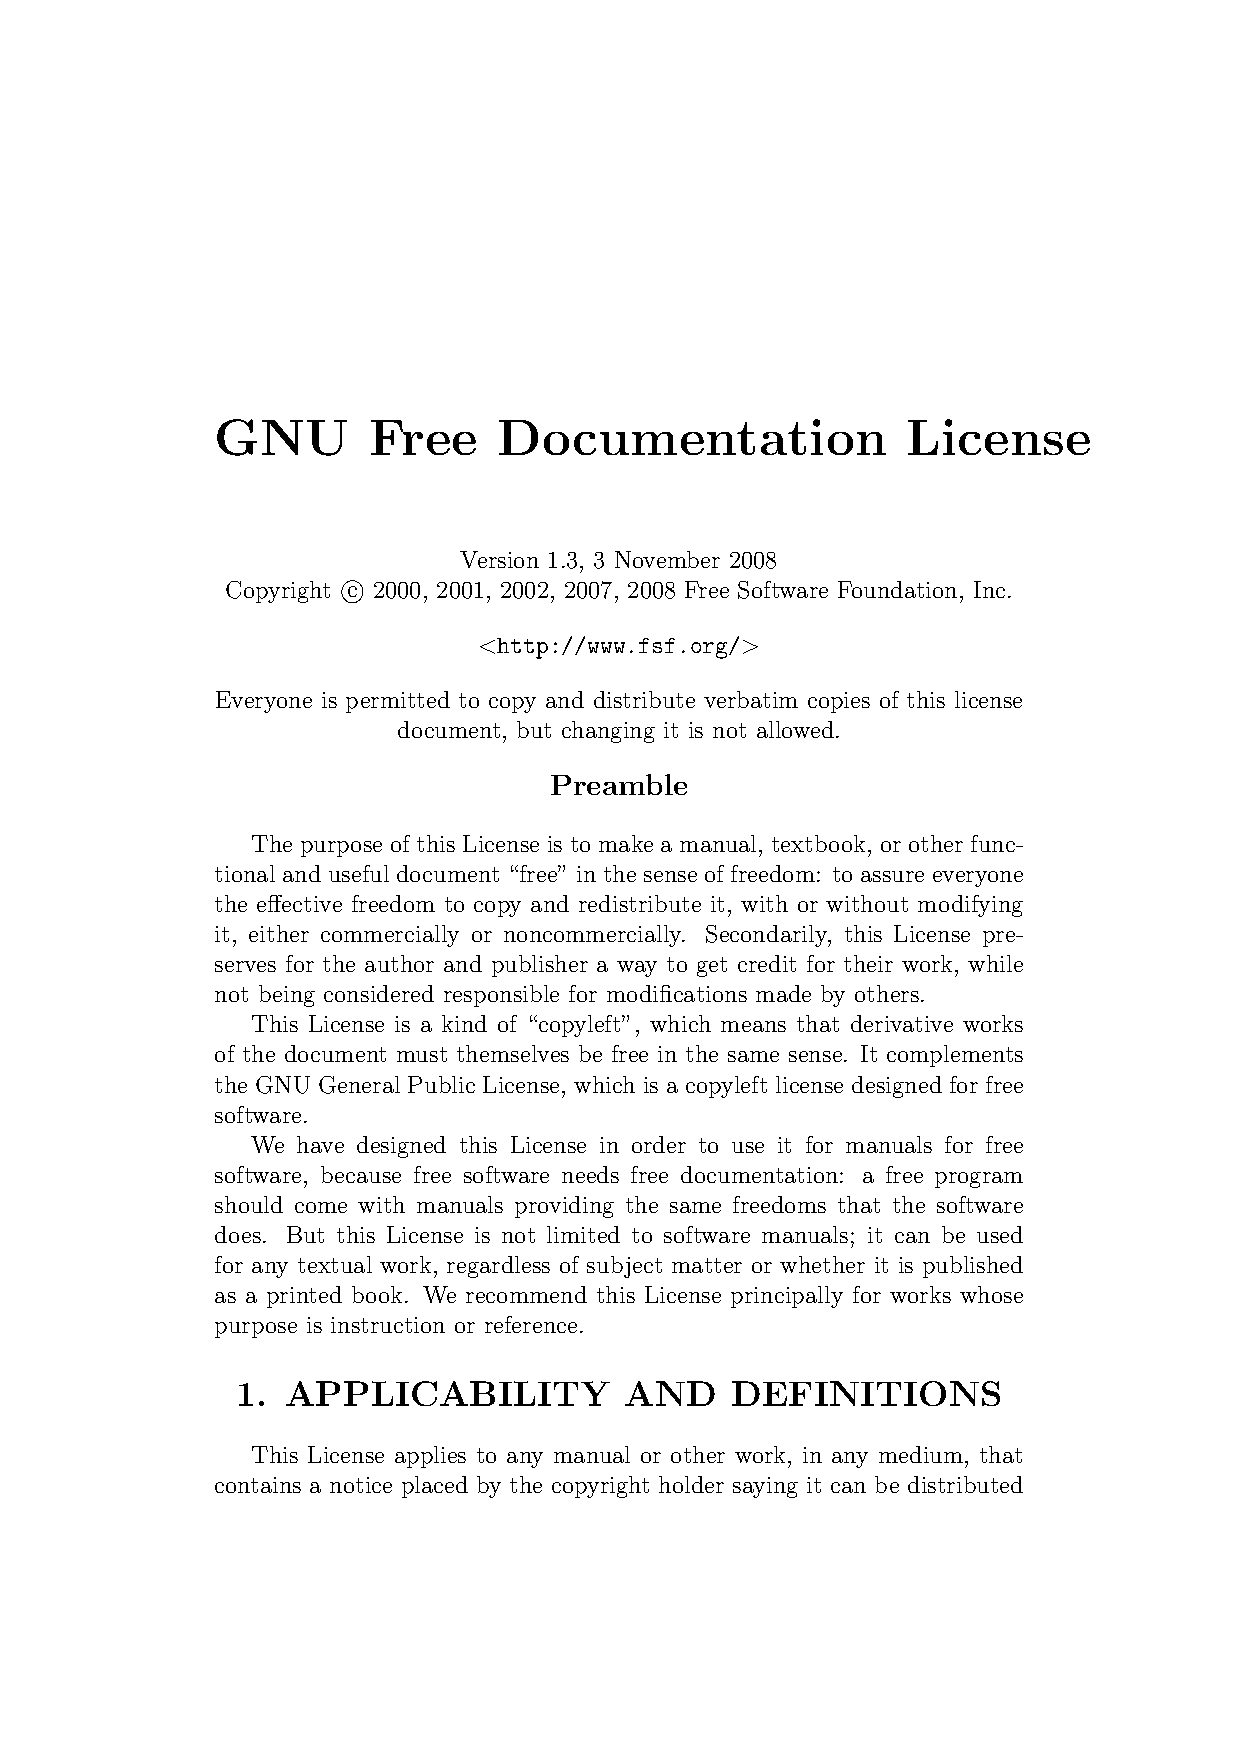
\includepdf[pages={1-10}, pagecommand={}]{gfdl.pdf}

\begin{comment}


\chapter{Proof that $S_0$ is trivial}

By definition, $S_0$ is the set of permutations of the empty set, that is, the set of all bijections from $\emptyset$ to $\emptyset$.  If we go back to the true definition of a function, we recall that a function from a set $A$ to itself is a relation $f$ on $A$ (that is, a subset of $A \times A$) such that for each $a\in A$, there is a unique $b\in A$ such that $(a,b)\in f$.

So let A be the empty set.  Then $A \times A$ is also the empty set (do you see why?). Now,  $f=\emptyset$ is a subset of $A \times A$, and it is vacuously true that $f$ has the property that for each $a\in A$, there is a unique $b\in A$ such that $(a,b)\in f$ (it is vacuously true since there are no elements of $A$).  So $f$ is a function from $A$ to $A$. Since there is no other subset of $A \times A$, $f$ is the only function from $A$ to $A$.

The remaining question is: Is  $f$ a permutation on $A$; that is, is $f$ a bijection?  The answer is yes: $f$ is both vacuously onto and vacuously one-to-one.  So there is a unique bijection from $\emptyset$ to $\emptyset$. Formally, it's the subset $\emptyset$ of $\emptyset \times \emptyset$.  Informally, it's the unique map that doesn't send anything anywhere.

Thus, $S_0$ contains exactly one element, and hence is the trivial group.
\end{comment}
%%%%%%%%%%%%%%%%%%%%%%%%%%%%%%%%%%%%%%%%%%%%%%
% \printsolutions[chapter=1]


\begin{thebibliography}{99}

\bibitem{F} John B. Fraleigh, \textit{A First Course in Abstract Algebra (7th ed.)}, Addison Wesley, 2002.

\bibitem{J} Thomas W. Judson, \textit{Abstract Algebra: Theory and Applications}. Revised edition published under the GNU Free
Documentation License, 1997 (revised 2016). \url{
http://abstract.pugetsound.edu/}

\bibitem{NZM} Ivan Niven, Herbert S. Zuckerman, and Hugh L.
Montgomery. \textit{An Introduction to the Theory of Numbers (5th
ed.)}, John Wiley \& Sons, 1991.

\end{thebibliography}

\end{document}